\documentclass[10pt]{report}
\usepackage[utf8]{inputenc}
\usepackage[italian]{babel}
\usepackage{multicol}
\usepackage[bookmarks]{hyperref}
\usepackage[a4paper, total={18cm, 25cm}]{geometry}
\usepackage{graphicx}
\usepackage{xcolor}
\usepackage{textcomp}
\graphicspath{ {./img/} }
\usepackage{listings}
\usepackage{makecell}
\usepackage{qtree}
\usepackage{pgfplots}
\usepackage{tikz}
\usepackage{amsmath}
\usepackage{cancel}
\usepgflibrary{shapes}
\usepgfplotslibrary{fillbetween}
\definecolor{backcolour}{RGB}{255,255,255}
\definecolor{codegreen}{RGB}{27,168,11}
\definecolor{codeblue}{RGB}{35,35,205}
\definecolor{codegray}{RGB}{128,128,128}
\definecolor{codepurple}{RGB}{205,35,56}
\lstdefinestyle{myPython}{
	backgroundcolor=\color{backcolour},   
	commentstyle=\color{codegreen},
	keywordstyle=\color{codeblue},
	numberstyle=\tiny\color{codegray},
	stringstyle=\color{codepurple},
	basicstyle=\small\ttfamily,
	breakatwhitespace=false,         
	breaklines=true,                 
	captionpos=b,                    
	keepspaces=true,                 
	numbers=left,                    
	numbersep=2pt,                  
	showspaces=false,                
	showstringspaces=false,
	showtabs=false,                  
	tabsize=2,
	language=python
}
\newcommand*\triangled[1]{\tikz[baseline=(char.base)]{
            \node[regular polygon, regular polygon sides=3,draw,inner sep=1pt] (char) {#1};}}
            
\usepackage{fancyhdr}
\pagestyle{fancy}
\renewcommand{\headrulewidth}{0pt}
\fancyhead{}
\fancyfoot[L]{Telegram: \texttt{@fexed}}
\fancyfoot[R]{Github: \texttt{fexed}}
\begin{document}
\title{Algorithm Engineering}
\author{Federico Matteoni}
\date{A.A. 2021/22}
\renewcommand*\contentsname{Index}

\maketitle
\tableofcontents
\pagebreak
\section{Introduction}
Teacher: Paolo Ferragina\\
Exam: written + oral. Midterms in November and December, with exercises.\\
Classes will be recorded on Microsoft Teams. Also the book "The Magic of Algorithms" is very important: you must be used to talk about these things, not just be able to solve exercises.
\paragraph{Course} \textbf{Design} and \textbf{analysis} of algorithms but also insights about \textbf{implementation}, with reference to libraries and considerations about what happens when using certain algorithms. The use case is \textbf{big data}.
\subsection{Algorithms} 
\paragraph{Algorithms} Knuth's definition: "\textit{a finite, definite, effective procedure that takes some input and returns an output, with the output being the answer to the problem you want to solve}."\begin{list}{}{}
	\item \textbf{Finite}: a \textbf{finite sequence of steps}, not only a finite numbers of operations but also \textbf{the algorithm must terminate}. \texttt{while (true) do ...} will go on forever, so it's not an algorithm. The number of steps must be \textit{very definite and reasonable}, which relates to the efficiency of the algorithm.
	\item \textbf{Definite}: the steps are definite in an unambiguous way.
	\item \textbf{Effective}: every step is basic, atomic, something that we can execute in small or constant time, constant is not a very precise word (seconds? Milliseconds?) so we will accept the "small time" rough definition. Also, the mapping input $\rightarrow$ output must always be correct, which is the biggest difference with IA. An algorithm outputs the correct output for each input.
\end{list}
\paragraph{RAM} Random Access Machine, CPU $\leftrightarrow$ M, classical computing model (Von Neumann machine), the memory can read any place in constant time.\\
We will make a more sophisticated step, but without presenting very complicated models. We need a good balance, not a perfect but a \textit{better} approximation than the RAM.
\paragraph{Analysis} Let's take an algorithm A and let's find a function $T_A(n)$ that describes the time complexity of A. $n$ is the input size, the number of items that the algorithm has to process. The time that A will take will be in hours, seconds or milliseconds based on the machine, but we approximate that time taken with the number of steps that are computed. Also, the number of steps depends not only on the number of items but on the items themselves, too. So we usually analyze the worst case scenario, or less often the average scenario. By analyzing the worst case scenario we can figure out the worst or "maximum" number of steps. \textbf{Asymptotic analysis}.\\
We want to exploit the characteristics of the various types of memory.
\subsection{2-Level Memory Model}
We will count not all the steps but the I/O ops, with a \textbf{2-level memory model}: the \textbf{first level} is the \textbf{internal fast memory} (cache + RAM) and the \textbf{second level} is the \textbf{mass unbound memory} (disk). In small memory situations, the first level can be interpreted as cache and the second level as internal memory, other times the first level is the internal memory and the second level is unbound slow memory.
\begin{list}{}{}
	\item \textbf{Spatial Locality}: access near items
	\item \textbf{Temporal Locality}, or small working set: far apart items used often so we can exploit their presence in the cache
\end{list}
\paragraph{Poly vs Exp time complexity} Let's say we have three algorithms with $n$, $n^2$ and $2^n$ in time complexity respectively. Let's \textbf{express the time complexity fixing $t$ time and counting how many items we can process in $t$ time}.
\begin{list}{}{}
	\item A linear algorithm $O(n)\Rightarrow n = t$
	\item A quadratic algorithm $O(n^2)\Rightarrow n = \sqrt{t}$
	\item An exponential algorithm $O(2^n)\Rightarrow n = \log_2(t)$
\end{list}
\pagebreak
With a $k$ times faster machine, we can imagine that we're using $k$ original machines in parallel. In this case:
\begin{list}{}{}
	\item With a linear algorithm on a $k$ times faster machine $\Rightarrow n = kt$\\
	The \textbf{linear algorithm takes full advantage of the faster machine}
	\item With a quadratic algorithm on a $k$ times faster machine $\Rightarrow n = \sqrt{kt}$\\
	The \textbf{quadratic has a small advantage of a multiplicative factor} $\sqrt{k}$
	\item With an exponential algorithm on a $k$ times faster machine $\Rightarrow n = \log_2(kt)$\\
	The \textbf{exponential algorithm has a negligible advantage of a sum factor} $\log_2 k$, basically none
\end{list}
\paragraph{Example} We have an integer array $A[1, n]$, of which we want to compute the sum, so $n$ items.
\begin{list}{}{}
	\item First approach: load $B$ items and process them, then load the next $B$ items and process and so on\ldots\\
	We do \#I/O = $\frac{\displaystyle n}{\displaystyle B}$: this is called the \textbf{scan cost}, we need to see each element in batches of $B$ elements, so $B$ is the \textbf{size of the memory page}.
	\item We can follow a different approach: take the first item of each batch of $B$ elements, then the second items and so on\ldots\\
	This will take $n$ steps, but it could be slower because we \textbf{do more I/O operations} (\#I/O = $n$).\\
	\textbf{The larger the jumps the more I/O operations we do}, because this model doesn't distinguish between local and random I/Os.
\end{list}
\paragraph{Binary Search} We have an array of $n$ elements. We pick the middle element, we go to left or right based on the comparison result, take the middle element of the chosen section and so on\ldots\\
The time complexity is $T(n) = O(\log_2 n)$, but \textbf{we have a lot of I/Os} and big jumps, meaning elements in different and far apart pages.\\
At a certain point the sub array where we search will be smaller than a page, so we have $$\underset{\text{Steps}}{\underbrace{\log_2 n}} - \underset{\text{Last page}}{\underbrace{\log_2 B}} = \log_2 \frac{n}{B}$$
This means that \textbf{the larger the page the smaller the number of I/Os}.
\subparagraph{Small note} One consideration: $n$ is the number of items while $B$ is in kilobytes. If we consider integers of 8 bytes, we have $\frac{\displaystyle B}{\text{size}}$ items, and with $B = 32 \text{ KB} = 2^{15}\text{ KB}$ we have circa 4000 items, or $\frac{\displaystyle 2^{15}}{\displaystyle 2^3} = 2^{12}$.
\paragraph{Improving Binary Search} We can consider the $B^+$-trees. We sort the array in ascendant order and split it into portions of the page size $B$. The splits are called leafs, and each leaf has a key (one of the elements). We build a page with each key and the next element is the pointer to its page. Above one level, a page with a key of the first key list and a pointer to the key list, a key of the second and so on\ldots\\
We fetch a page, perform binary search and follow the pointer. \#I/Os $=\log_B \frac{n}{B}$ and the number of steps is a binary search for every page, so $$\underset{\text{Pages}}{\underbrace{\log_B \frac{n}{B}}} \cdot \underset{\text{BS in each page}}{\underbrace{\log_2 B}}$$
\begin{center}
	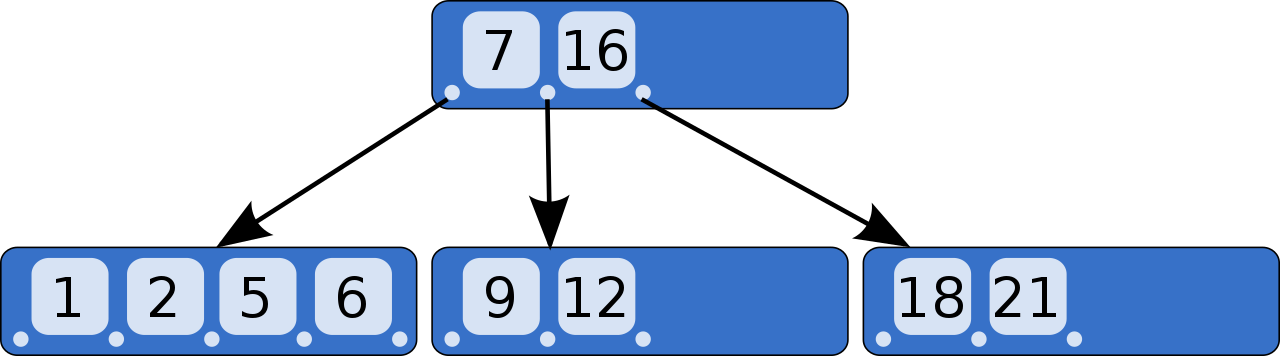
\includegraphics[scale=0.25]{2.png}
\end{center}
\subparagraph{Analysis} Let's say that the elements are $n = (1 + \epsilon)M$ with $\epsilon > 0$ data outside of the memory: $M$ is totally full and $\epsilon M$ elements are stored in the unbound memory.\\
Let's find the probability of accessing the disk. With a totally random algorithm, we have $$P(\text{Accessing the disk}) = P(\epsilon) = \frac{\epsilon M}{n} = \frac{\epsilon\cancel{M}}{(1 + \epsilon)\cancel{M}} = \frac{\epsilon}{1 + \epsilon}$$
Let's compute the average time of a step. We can say the the time of a computing step is $1$, but time varies in case of memory access. We have three types of steps: computing step (costs $1$), internal memory access  (costs $1$ as well) step or disk access step (larger, let's say that it costs $c$). Let's suppose that the probability of accessing the memory is $a$, then the average of $X$ variable denoting time of a step is:
$$E[X] = \sum_x P(X=x) = \underset{\text{Computing step}}{\underbrace{(1-a)\cdot 1}} + \underset{\text{Memory access step}}{\underbrace{a(\overset{\text{External memory}}{\overbrace{P(\epsilon)\cdot c}} + \overset{\text{Internal memory}}{\overbrace{(1-P(\epsilon))\cdot 1}})}}$$
$0 < a < 1$ and $1 - P(\epsilon)$ are very small, so we can rewrite

$$E[X] = \cancel{(1-a)} + a(P(\epsilon)c + \cancel{(1-P(\epsilon))}) = a\cdot P(\epsilon)\cdot c = a \cdot \frac{\epsilon}{1 + \epsilon} \cdot c + O(1)$$
If $a = 0$ then there is no memory access so the cost is constant. The larger is $a$ the more memory accesses there are, the more that term is important, which is exactly what we want to capture. Usually, $a = 0.3 = 30\%$ and $c = 10^6$ the gap between accessing the disk and accessing the internal memory.\\
So $\frac{\epsilon}{1 + \epsilon}\cdot 0.3 \cdot 10^6 = \frac{\epsilon}{1 + \epsilon} \cdot 300000$. If $P(\epsilon) = 0.001$ the avg time of a step is $0.001 \cdot 300000 = 300$, so the disk has a lot of impact even with only a thousandth of memory access being on disk: the avg cost is 300 and not 1.
\section{Sorting}
\subsection{Permuting} Given an array $S[1, m]$ and a permutation $\pi$, the permutation problem asks to permute $S$ according to $\pi$, creating $[S[\pi[1]], S[\pi[2]],\ldots,S[\pi[m]]$. For example $S = [A, B, C, D], \pi = [3, 1, 2, 4]$ then $\pi$ tells that the $\pi[0] = 3$ item goes to the first position. So $S_\pi = [C, A, B, D]$
\begin{lstlisting}[style=myPython]
for i = 1 to n:
	S1[i] = S[pi[i]]
\end{lstlisting}
Which costs $\Theta(n)$
\begin{center}
	\begin{tabular}{c | c | c}
 & PERM & SORT \\
\hline
RAM & $n$ & $n\log n$\\
\hline
2-level memory & min\{$n$, $C_{sort}$\} & $C_{sort}$
\end{tabular}
\end{center}
Solving the permuting in a scan + sort kind of way, otherwise we have to do a disk access per value.\\
\begin{list}{}{}
	\item \textbf{Scan} S : $\langle\text{S}[i], i\rangle$ which is $\langle\text{item}, \text{position}\rangle \Rightarrow \langle\text{A}, 1\rangle, \langle\text{B}, 2\rangle, \langle\text{C}, 3\rangle, \langle\text{D}, 4\rangle$ (Costs $O(\frac{n}{B})$)
	\item \textbf{Scan} $\pi$ : $\langle\pi[i], i\rangle$ which is $\langle\text{source}, \text{destination}\rangle \Rightarrow \langle3, 1\rangle,\langle1, 2\rangle,\langle2, 3\rangle,\langle4, 4\rangle$ (Costs $O(\frac{n}{B})$)
	\item \textbf{Sort $\langle\pi[i], i\rangle$ by first component} $\Rightarrow \langle1, 2\rangle, \langle2, 3\rangle, \langle3, 1\rangle, \langle4, 4\rangle$ (Costs $O(C_{\text{sort}})$)
	\item \textbf{Parallel scan} $\begin{array}{l}
	\langle\text{A}, 1\rangle, \langle\text{B}, 2\rangle, \langle\text{C}, 3\rangle, \langle\text{D}, 4\rangle\\
	\langle1, 2\rangle, \langle2, 3\rangle, \langle3, 1\rangle, \langle4, 4\rangle
	\end{array}\Rightarrow \langle\text{A}, 2\rangle, \langle\text{B}, 3\rangle, \langle\text{C}, 1\rangle, \langle\text{D}, 4\rangle$ (Costs $O(\frac{n}{B})$)
	\item \textbf{Sort by second component} $\Rightarrow\langle\text{C}, 1\rangle,\langle\text{A}, 2\rangle,\langle\text{B}, 3\rangle,\langle\text{D}, 4\rangle$ (Costs $O(C_{\text{sort}})$)
	\item \textbf{Scan} $\Rightarrow$ [C, A, B, D] (Costs $O(\frac{n}{B})$)
\end{list}
I/O cost $=$ 4 scan + 2 sort $= O(\frac{n}{B}) + O(C_{sort})$ sorting cannot cost less than $\frac{n}{B}$ so $O(C_{sort})$
\pagebreak
\paragraph{Bounds} So \textbf{we have proposed upper-bounds}, hence algorithms, \textbf{for the sorting and the permuting problem}. The permuting problem can be solved in $O(\frac{n}{B}) + O(C_{sort})$ I/Os, while moving $n$ items takes $\Theta(n)$ I/Os.\\
Sorting $n$ items in a two level memory, with size $M$ for internal memory and $B$ for the disk page size, costs $O(\frac{n}{B} \cdot \log_{\frac{M}{B}} \frac{n}{M})$ with $L = \log_{\frac{M}{B}} \frac{n}{M}$ often written as $\overline{O}(\frac{n}{B})$ with the overline or over tilde that means that is a scan.\\
$L$ consists of the base $\frac{M}{B}$ and the argument $\frac{n}{B}$ which means that with a larger memory I'd like it to be faster, with bigger $M$ the argument decreases and the base increases so the logarithm shrinks a lot. With a bigger $B$ page size, $\frac{n}{B}$ decreases but the base increases.\\
$\frac{\displaystyle M}{\displaystyle B} =$ how many pages I can keep in the internal memory. Let's say $n = 2^{40}$, $M = 8 \text{Gb} = 2^{33}$ and $B = 32 \text{Kb} = 2^{15}$, then $$\log_{\frac{M}{B}} \frac{n}{M} = \frac{\log_2\frac{n}{M}}{\log_2 \frac{M}{B}} = \frac{\log_2 \frac{2^{40}}{2^{33}}}{\log_2 \frac{2^{33}}{2^{15}}} = \frac{\log_2 2^7}{\log_2 2^{18}} = \frac{7}{18} < 1$$
Let's see when is sorting preferred to moving items or viceversa
$$\frac{n}{B} \log_{\frac{M}{B}} \frac{n}{M} < n \Leftrightarrow \log_{\frac{M}{B}} \frac{n}{M} < B$$\\
We have $B = 1$ in the RAM model, $B = 32$Kb in the 2-level model compared to $\log_{\frac{M}{B}}\frac{n}{M} = 2$ or $3$. In practical situations with disk, sorting is better than moving numbers. If $B = 1$, in the RAM model, $M = O(1)$, then sorting is worse than moving.
\subsection{Sorting} Let's consider binary merge sort, which in the worst case costs $O(n\cdot \log_2 n)$.
\begin{lstlisting}[style=myPython]
def MergeSort(S, i, j):
	# sort if at least two items, otherwise already sorted
	if (i < j):
		m = (i+j)/2
		MergeSort(S, i, m-1)  # split into two halves
		MergeSort(S, m, j)
		Merge(S, i, m, j)  # most of the cost is here
\end{lstlisting}
Let's evaluate the I/Os in the case that $n >> M$, meaning that \textbf{the array can't be stored entirely in internal memory}. Since it's \textbf{based on the merge procedure}, we can evaluate the cost of the merge and multiply by the number of levels.\\
It loads a page every time it needs it and writes a pages every time it fills one. So if the two arrays to merge are long $l$, it makes $\frac{l}{B}$ I/Os. So it takes \#I/Os $=O(\frac{n}{B} \log_2 n)$: we partition $n$ elements in $\log_2 n$ halves and merge each.\\\\
\textbf{Sorting} consists of \textbf{computing the sorted permutation} and \textbf{implementing the sorted permutation}. So we can say that sorting $\geq$ permuting, is at least difficult as permuting.\\
In the RAM model the $\geq$ is $>$, it's strict, because sorting is $n\cdot\log n$ and computing the sorted permutation is the real bottleneck, because implementing it is linear. In the 2-level memory model they are almost equivalent. This considering \textbf{atomic items}, integers o non-splittable strings.\\
\textbf{The mismatch is the base of the logarithm}. The binary merge sort is $O(\frac{n}{B} \log_2 \frac{n}{M})$: partitioning the array in blocks of size $M$, the size of the memory, called runs. Can we generate runs longer than M in few I/Os? On average we will be able to create runs of size $2M$, which saves 1 full scan of data (which, for large data, is a lot of time saved).
\subsection{Snow Plow Algorithm} Sort the items that you can, leave item that you cannot.
\paragraph{Example}
$S = 1, 7, 5, 3, 2$, with $M = 3$ items.\\
The \textbf{memory is divided in two parts}: a \textbf{min heap, items that are still unsorted}, and an \textbf{unsorted part, the "snow that we cannot clean"}.\\
We start by \textbf{loading $M$ items}, which will \textbf{all go in the unsorted part}: 1, 7, 5. We \textbf{sort them}, moving each to the min heap with the unsorted part left empty. Then we \textbf{pick the minimum element and write it out} of the memory: we have emptied a position, and we can fetch another item: the 3. The new item is compared to the current minimum, the written-out element. 3 is larger than the current minimum, so is written inside the min heap, which is now 3, 5, 7. We write again out the minimum, 3, and fetch another item. 2 is smaller than 3, so it goes in the unsorted part. At some point the min heap will be empty, the unsorted part will be full and we restart the phase. We pay 1 I/O as soon as we write out $B$ items.
\begin{center}
	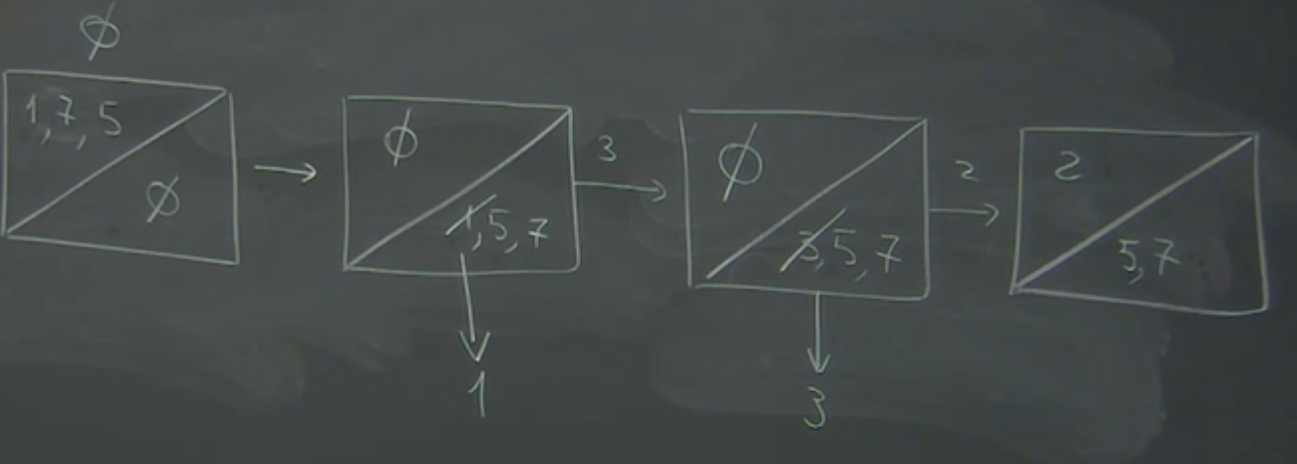
\includegraphics[scale=0.5]{1.png}
\end{center}
\begin{lstlisting}[style=myPython]
U = unsorted array of M items  # load the first M items
H = min-heap over items of U  # we sort them and put in the min heap
U = {}
while H != {}:
	min = minimum from H
	min -> output run  # write out the minimum
	next = next item from input sequence  # fetch another item
	if next < min:  # if it's smaller
		next -> U  # it goes in the unsorted part
	else:
		next -> H  # otherwise it goes in the min heap
\end{lstlisting}
Let's \textbf{prove that the runs are 2M on average}.\\
We start with $|U| = M$ and $|H| = 0$, with $U$ unsorted part and $H$ min heap part. As the algorithm goes on, we read some items: $\tau =$ \# items read. The phase has processed $\tau + M$ items: $\tau$ read items and $M$ that were already in memory.\\
At the end of the phase, $|H| = 0$ and $|U| = M$ with $\tau$ items written out: $\tau$ is the \textbf{length of the run}, we have to compute it by making hypothesis about the distribution of the items, hence the probabilities of going to $U$ and $H$. Let's say that $P(\text{item read goes to }U) = \frac{1}{2}$, a totally random sequence (by changing the probability we change "how much sorted" is the sequence, and the more sorted is the sequence, the smaller the probability of going to $U$)\\
$E[|U|] = \frac{\tau}{2}$ because we have $\tau$ items that go to $U$ with probability $\frac{1}{2}$. Given that $|U| = M$, then $$E[|U|] = \frac{\tau}{2} = M \Leftrightarrow \tau = 2M$$ so average $\tau = 2M$
\paragraph{Exercise} $M = 2$ and $S = 1, 8, 3, 2, 5, 0, 4, 6$\ldots\\
$\left[\begin{array}{l r}
1,8&\\
&\emptyset
\end{array}\right]\rightarrow\left[\begin{array}{l r}
\emptyset&\\
&\not1,8
\end{array}\right]\rightarrow\left[\begin{array}{l r}
\emptyset&\\
&\not3,8
\end{array}\right]\rightarrow\left[\begin{array}{l r}
2&\\
&\not8
\end{array}\right]\rightarrow\left[\begin{array}{l r}
2,5&\\
&\emptyset
\end{array}\right]$ first run is $1,3,8$\\
$\left[\begin{array}{l r}
2,5&\\
&\emptyset
\end{array}\right]\rightarrow\left[\begin{array}{l r}
\emptyset&\\
&\not2,5
\end{array}\right]\rightarrow\left[\begin{array}{l r}
0&\\
&\not5
\end{array}\right]\rightarrow\left[\begin{array}{l r}
0,4&\\
&\emptyset
\end{array}\right]\rightarrow$ second run is $2,5$\\
$\left[\begin{array}{l r}
0,4&\\
&\emptyset
\end{array}\right]\rightarrow\left[\begin{array}{l r}
\emptyset&\\
&\not0, 4
\end{array}\right]\rightarrow\left[\begin{array}{l r}
\emptyset&\\
&\not4, 6
\end{array}\right]\rightarrow\left[\begin{array}{l r}
\emptyset&\\
&\not6
\end{array}\right]\rightarrow$ third run is $0,4,6$
\paragraph{Issues} Binary Mergesort doesn't always exploit all the memory. Because after creating the $M$-long first runs, for the merge we need $3B$ for reading the memory (one for the first run, one on the second run and one page for the output), and $3B << M$: a lot of unused memory. We could fetch 2 pages per run, but the second page can be used only after the first page, so no advantage in allocating all data. Since there's a sequence of processing, even if we immediately load all the pages, we do not have much advantage in doing so. So \textbf{we would like to merge $k$ runs instead of two runs at a time}.
\pagebreak
\paragraph{$k$-way Mergesort} Since we want to fill the memory, we want $(k+1)B = M$: $k$ pages of size $B$ needed for $k$ runs plus $1$ output page of size $B$. So $k = \frac{M}{B} - 1 \simeq \frac{M}{B}$ pages.\\
Each run has $l$ elements, but for the merge we can load just $B$ elements per run: the runs are sorted, so every time we merge $B$ elements from a run we load another page from the same run (keeping track of which elements belongs to each run with a $\langle\text{elem}, \text{run}\rangle$ min heap). When we fill the output page (of size $B$) we write it out and empty the page. \textbf{This generates $\frac{l}{B}$ I/Os per run during the merge procedure} (and the merged run is long $k\cdot l$ elements).\\
The array of size $n$ is divided into blocks of size $M$, which are sorted: this takes $\frac{M}{B}$ I/Os, for $\frac{n}{M}$ runs. So the \textbf{total cost for creating runs is $O(\frac{n}{\cancel{M}} \cdot \frac{\cancel{M}}{B}) = O(\frac{n}{B})$}.\\
Then \textbf{we merge $k$ runs at the time}: the cost is linear for every run of size $l$, and we can produce $\frac{n}{l}$ runs, so a \textbf{total cost of $\frac{\cancel{\:l}}{B}\cdot\frac{n}{\cancel{l\:}} = \frac{n}{B}$ I/Os}.\\
The merge tree has $\frac{n}{M}$ leafs and every node has $k$ runs to merge from the lower level, making it \textbf{$\log_k \frac{n}{M}$ levels high}.\\\
The cost of merge sort is $$O\left(\underset{\text{Creating the runs}}{\underbrace{\frac{n}{B}}} + \underset{\text{Single merge}}{\underbrace{\frac{n}{B}}}\cdot\underset{\text{Total merges}}{\underbrace{\log_k \overset{\text{Leafs}}{\overbrace{\frac{n}{M}}}}}\right)$$ which we have seen with $k = \frac{M}{B}$.\\
With improved $B$ and $M$ by compression. So 3, 5, 10 is written as 3 (the first item) and storing the gaps (gap encoding) so 2, 5,\ldots with variable length encoders.
\paragraph{More disks} Let's rewrite the bound
$$\frac{n}{B}\cdot\log_{\frac{M}{B}}\frac{n}{M}$$
We don't know how items are consumed on the disks, given $D$ disks. With $k = 2, D = 2$ we can take advantage of the parallelism on the first load. But once loaded in memory, we may consume the pages asymmetrically, so we may end up reading a lot from a disk and very few times from the other. Possibly, every page on the first disk is used before the second page on the second disk. So by adding more disks we take full advantage because they are the denominators. The known optimal bound is:
$$\Theta\left(\frac{n}{BD}\cdot\log_{\frac{M}{B}}\frac{n}{BD}\right)$$
For 1 disk is $O(\frac{n}{B}\cdot\log_{\frac{M}{B}}\frac{n}{B})$\\
For $D$ disks we can consider one big disk with $B' = D\cdot B$ page size, so the heads of the disks are fixed together and move together. We do not change the algorithm, so the complexity is simply $$O\left(\frac{n}{B'}\cdot\log_{\frac{M}{B'}}\frac{n}{B'}\right) = O\left(\frac{n}{DB}\cdot\log_{\frac{M}{DB}}\frac{n}{B'}\right)$$ With D in the base of the logarithm reducing it, making the value larger, but the impact is small and the simplicity of the management with this method makes it worth it. This is called \textbf{disk striping}.
\paragraph{Binary Decision Trees} Every node $(a,b)$ generates a comparison, the left branch is followed if $a<b$ and the right if $a>b$: it \textbf{represents an algorithm}. The \textbf{leafs are sorted permutations according to the path of comparisons}, total number of leafs is $n!$. The question is how big should be the tree so that it's a sorting algorithm, so to reach a number of leafs that's at least $n!$, the number of possible permutations of $n$ elements? It grows by $2^t$ nodes for every level $t$, so $2^t > n!$ and we have the lower bound.\\
The left subtree, where the comparison is $a < b$, simply generates (by following a path) all the permutations in which $a$ comes before $b$, whatever number of elements are between them. The right path, vice versa, generates permutations where $b$ comes before $a$.
\subparagraph{Lower bounds} Binary decision trees provide a lower bound of sorting in the RAM model. Now let's see the I/O lower bound, so not counting comparisons but read/written pages.\\
The main idea is that \textbf{whenever I fetch a page I fetch $B$ items}, not just two, so we can do many comparisons before loading another page. And the page goes in internal memory where there are more items which we compare. Whenever the items goes to internal memory we have to avoid repeating comparisons.\\
The memory $M$ consists of several items. When we bring the page of size $B$ in internal memory, we already have $M-B$ other items in the memory. So with one I/O we can execute many comparisons. If $B = 1$ and $M - B = 3$, so 3 items in $M$ and 1 item brought from disk. We can assume that the items in memory are sorted, so the item brought can go in 4 position (before the first, between the first two\ldots).\\
In general, the $B$ items can enter the $M-B$ items in $n$ ways. The memory consists of $M$ cells, so $n = \left(\begin{array}{c}
M\\B
\end{array}\right)\cdot B!$ with $B!$ because we have to account for the shuffling, but it needs to be counted only once when the items are first loaded. We have $\left(\begin{array}{c}
M\\B
\end{array}\right)$ because every item from $B$ can be inserted in one slot of $M$ possible slots, so $B$ slots out of $M$.\\
Making $t$ I/Os, each can be a new or an old read: either one of the $\frac{n}{B}$ pages for the first time or any other page (or one of those pages for the second/third/\ldots time). So two situations \begin{enumerate}
	\item \textbf{A new read}, a read of an input page for the first time: \# new reads = $\frac{n}{B}$
	\item \textbf{An old read}, all other read-cases: \# old reads = $t - \frac{n}{B}$
\end{enumerate}
Two kinds of nodes, one node refers to a new I/O the other to an old I/O.\\
In a new I/O we have $\left(\begin{array}{c}
M\\B
\end{array}\right)\cdot B!$ options, accounting for the shuffling, in the second case we have $\left(\begin{array}{c}
M\\B
\end{array}\right)$ options.\\
In any path $\frac{n}{B}$ are new reads and $t - \frac{n}{B}$ are old. \textbf{For this tree to be a sorting algorithm, the number of leafs must be $\geq n!$}. Each node is no longer binary and can be one of two kinds: it's still a decision tree.\\
The number of permutations that the algorithm can distinguish is $$\#\text{ permutations}= \underset{\text{New I/Os}}{\underbrace{\left( \left(\begin{array}{c}
M\\B
\end{array}\right)\cdot B!\right)^{\frac{n}{B}}}}\cdot \underset{\text{Old I/Os}}{\underbrace{\left(\begin{array}{c}
M\\B
\end{array}\right)^{t - \frac{n}{B}}}} = \left(\begin{array}{c}
M\\B
\end{array}\right)^{t}\cdot \left(B!\right)^{\frac{n}{B}} \geq n!$$
To compute, consider that $\log\left(\begin{array}{c}
a\\b
\end{array}\right) = b\log_2 \frac{a}{b}$ and solving for $t$ gives the multi way merge sort bound. $t = \Omega(\frac{n}{B}\log_{\frac{M}{B}} \frac{n}{M})$
\paragraph{Two sorting paradigms} The following:
\begin{list}{}{}
	\item \textbf{Merge-based} paradigm: partition (computationally free, $O(1)$), recursion, recombination (merge, $O(\frac{n}{B})$)
	\item \textbf{Partitioning-based} paradigm: partition (costly part, $O(n)$), recursion, recombination ($\not\exists$)
\end{list}
How can we design a multi way quick sort? We can't take one pivot, because that'll be binary. We can take many pivot but we have to guarantee a good usage of internal memory, but more importantly we need that the partition have to balanced: with $k$ pivot I'd like that every partition has $\frac{n}{k}$ items. This requires a theorem.\\
Let's refresh the quick sort. %TODO
\paragraph{Time complexity of quick sort is $O(n\cdot\log n)$ on average} Let's prove it by introducing a random variable. $$X_{u,v} = \left\{\begin{array}{c l}
1&\hbox{if }S[u]\hbox{ is compared to }S[v]\\0&\text{else}
\end{array}\right.$$ and we want the average number of comparisons $$E\left[\sum_{u=1}^m\sum_{v>u}^m X_{u,v}\right] = \sum_{u=1}^m\sum_{v>u}^m E\left[X_{u,v}\right] = $$
The average of an indicator value (which $X_{u,v}$ is) is the sum of all possible values times their probability $$= \sum_{u=1}^m\sum_{v>u}^m \left(1\cdot P(S[u]\text{ is compared to }S[v]) + 0\cdot P(S[u]\text{ is not compared to }S[v])\right) = $$
$$=\sum_u \sum_v P(S[u]\text{ is compared to }S[v])$$
Let's focus on the probability that taken two items they are compared. Comparison in quick sort is particular, may only occur in the partition part and when one of the elements is a pivot. With just one pivot and two parts, then $S[u]$ is compared to $S[v]$ only when one of them is the pivot. So $P(S[u]\text{ is compared to}S[v]) = P(S[u]$ or $S[v]$ is choosen as pivot in one call that involves both of them$)$
\begin{list}{}{}
	\item Case $a$: the pivot is smaller or greater than both items, so both items go to the same partition: not significative because they can be compared in the next time 
	\item Case $b$: the pivot is between the two items, so no comparison because they'll go to different partitions.
	\item Case $c$: is that one of the two items is taken as pivot, so \textbf{there's the comparison}.
\end{list}
So the probability is the number of times that $c$ can happen (two items, so $2$) divided by the total number of events possible, $b + c$, which is any item choosen between the two elements included, so $S[v] - S[u] + 1$. So $$P(S[u]\text{ is compared to }S[v]) = P(S[u]\text{ or }S[v]\text{ pivot in a call involving both}) = \frac{2}{S[v] - S[u] + 1}$$
So the formula becomes $$\sum_{u=1}^n \sum_{v>u}^n \frac{2}{S[v] - S[u] + 1} = 2\sum_{u=1}^n \sum_{k=2}^{n-S[u]+1} \frac{1}{k} \leq 2n\log n$$
\paragraph{$k$th ranked item} In unsorted array $S$, \textbf{the $k$th ranked item is the item that would go to the $k$th place if $S$ would be sorted}.\\
The obvious way: sort and pick the item in the position $k$, costing $n\cdot\log n$. This problem can be solved in $O(n)$ on average: same idea as quick sort with just one recursive call.\\
Pick a random pivot and do a \textbf{three-way partition}:
\begin{list}{}{}
	\item Partition of $n_<$ smaller elements than the pivot (unsorted)
	\item Partition of $n_=$ elements of the same value as the pivot (trivially sorted)
	\item Partition of $n_>$ larger elements than the pivot (unsorted)
\end{list}
If the elements falls into the middle partition we can immediately know which elements it is.\\
For example, $[3,2,0,\vline7,7,7,\vline10,8,9]$, if $k$ is 4 we can answer that, being that there are $3$ elements in the left partition, the 4th ranked element is a 7.\\
\textbf{If $k$ falls in the $=$ partition, I'm done}. \textbf{If it falls in one of the other two}, I don't yet know but we \textbf{can already discard some items}:
\begin{list}{}{}
	\item If the pivot is in the $<$ part we recurse on that part, with rank unchanged $k$
	\item If the pivot is on the $>$ part we recurse over there, in this case dropping from $k$ the items that are smaller: $k = k - (n_= + n_<)$
\end{list}
Only one recursive call.
$$T(n) = O(n) + [T(n_<)\text{ or }T(n_>)]$$
Depending on the choice of going to the left or to the right. Let's analyze that probabilities, supposing that $n_= = \frac{n}{3}$, a balanced partitioning, with the \textbf{pivot falling among the $n_=$ items} (the middle partition). This is the \textbf{good case}: the \textbf{pivot is between the position $\frac{1}{3}n$ and $\frac{2}{3}n$}, and happens with \textbf{probability $\frac{1}{3}$}. The \textbf{bad case is when we can only drop the pivot}, so we \textbf{recurse on the remaining $n-1$ elements}.\\
In the good case $n_< \leq \frac{2}{3}n$ and $n_> \leq 	\frac{2}{3}n$. So $$T(n) = O(n) + (P(\text{good case})\cdot T() + P(\text{bad case})\cdot T()) \Leftrightarrow$$
$$\Leftrightarrow T(n) = O(n) + \left(\frac{1}{3}\cdot T\left(\frac{2}{3}n\right) + \frac{2}{3}\cdot T(n - 1)\right) \Leftrightarrow$$
$$\Leftrightarrow T(n) \leq O(n) + \frac{1}{3}\cdot T\left(\frac{2}{3}n\right) + \frac{2}{3}\cdot T(n) \Leftrightarrow$$
$$\Leftrightarrow \frac{1}{3}T(n) \leq O(n) + \frac{1}{3}\cdot T\left(\frac{2}{3}n\right) \Leftrightarrow$$
$$\Leftrightarrow T(n) \leq O(n) + T\left(\frac{2}{3}n\right)$$
By applying the master theorem, we have that $T(n) = O(n)$.
\paragraph{Dual Pivot} \textbf{3-Way Partitioning} made with 2 pivot taken at random: it reduces the number of comparisons and it increases the number of swaps. This seems totally ineffective (\textbf{swaps impacts on memory} and \textbf{comparisons impact on CPU}), but the problem here is \textbf{mispredictions by the CPU}: modern CPUs do look-ahead in the computing and, if it badly predicts the future comparisons, it has to break the stack and go back. So with fewer comparisons it's better, it reduces the mispredictions: 10\% circa speed-up factor.\\
The pivots maintain an invariant:
\begin{list}{}{}
	\item First partition $[0, l-1]$: items $<p$
	\item Second partition $[l, k-1]$: items $p\leq \ldots\leq q$
	\item Third partition $[k, g]$: unprocessed items
	\item Fourth partition $[g+1, n]$: items $>q$
\end{list}
\begin{center}
	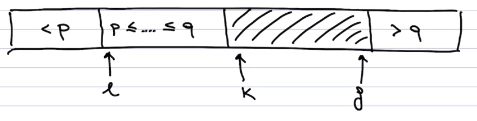
\includegraphics[scale=1]{7.png}
\end{center}
We take $S[k]$ and compare it to $p$. If $S[k]<p$ then swap (insert $S[k]$ in position $l$ and increase $l$).\\
Else, we compare $S[k]$ with $q$. If $S[k]\leq q$ we don't have to do anything, it's already in the correct position. Else, $S[k] > q$: we start from $g$ and go back until we find an element $\leq q$ and we swap $S[k]$ with that element.
\paragraph{Bounded Quick Sort} Bounding the recursive calls. Transform the deepness of the tree (the number of recursive calls) from $n$ to $\log n$, but the time complexity remains $n^2$ in the worst case.\\
The trick is \textbf{removing tail recursion}. Techniques applied by compilers, we'll do by hand.\\
\begin{center}
	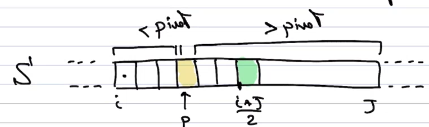
\includegraphics[scale=1]{8.png}
\end{center}
Let's see a generic call, between positions $i$ and $j$.\\
If $j - i > n_0$ (so if the remaining portion is sufficiently small, the array is in cache so we go fast) then we do insertion sort.\\
In the other case, with $\frac{i+j}{2}$ being the middle element, we do the partitioning: assuming the pivot on the left of the middle ($i \leq p < \frac{i+j}{2}$), the left partition of the pivot is smaller so contains less than half elements. So $i \leq p < \frac{i+j}{2}$, then recurse on the left because it has fewer elements, but we do not recurse on the right because it has a lot of elements so after the recursive call on the left we simply move $i$ by doing $i = p + 1$. Else, with $p$ on the right part, recurse on the right partition and then do $j = p-1$
\paragraph{Multi Way Quicksort} Key idea, given that we have a long array $S$ to be sorted and that doesn't fit in internal memory: we want to partition $S$ among $k$ buckets $B_1,B_2,B_3,\ldots,B_k$. Every bucket is associated to a pivot: $k-1$ pivots, a logical pivot $s_0 = -\infty$ at the beginning, $s_k = \infty$ at the end and $s_1,s_2,s_3,\ldots,s_{k-1}$ between the buckets.
$$B_i=\{S[j]\:|\: s_{i-1} < S[j] \leq s_i\}$$
So the "right" pivot is part of the bucket ($s_i \in B_i$). The goal is having balanced buckets $B_i \forall\:i$, so $|B_i| = \frac{\displaystyle n}{\displaystyle k}$.\\
The idea is similar to merge sort but in reverse: we use $k$ buckets of size $B$ in a memory of size $M$, so we want to guarantee that $k\cdot B \leq M$.
\pagebreak
\begin{enumerate}
	\item Sample at random $(a + 1)k - 1$ samples from $S$, the pivots $\Rightarrow A$\\
	This costs a scan, so $O(\frac{n}{B})$
	\item Sort the samples in $A$ so that $s_1<\ldots<s_{k-1}$\\
	All the pivots are in internal memory so it costs 0 I/Os.
	\item $s_i = A[(a+1)i]$\\
	Until the last block has $a$ items
	\begin{center}
		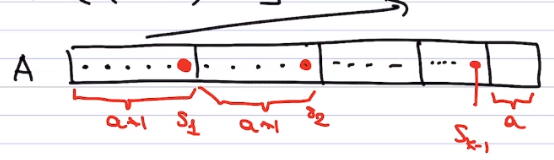
\includegraphics[scale=0.5]{3.png}
	\end{center}
	We sampled $(a+1)(k-1) + a = (a+1)k -1$ items
\end{enumerate}
If $a = 0$ the number of samples is $k-1$, no oversampling, fast sort ($O(k\log k)$) but no room to play around with the items. If $a > 0$ the sorting costs $O((ak)\log (ak))$. We chose $a = \Theta(\log k)$, only a logarithmic oversampling to get the balance $$a + 1 = 12\ln k$$
But we cannot assume that the memory can contain the $S$'s buckets, so  we fetch $B$ items from $S$ and distribute the items according to the pivots and do until a bucket is full. When a page is full, we write it as a page of the corresponding bucket (according to the pivot). This takes $O(\frac{n}{B})$ I/Os.\\
In total, $O(\frac{n}{B}) + \sum_{i=1}^k T(|B_i|)$ I/Os and balanced with $|B_i| \simeq \frac{n}{k}$ so $O(\frac{n}{B}) + \sum_{i=1}^k T(\frac{n}{k})$. If we solve the recursive call using a tree, like in quick sort, this becomes $O(\frac{n}{B}\log_k \frac{n}{B})$.\\
Balanced $\Rightarrow |B_i| < 4\cdot\frac{n}{k}$
\paragraph{Proof} By contradiction. We want to estimate $P(\exists\:B_i\:|\:|B_i|\geq \frac{4n}{k})$ and prove that it is $\leq \frac{1}{2}$ so that on average two extractions are enough to guarantee that one is correct.\\
$B_i = \{S[j]\:|\: s_{i-1} < S[j] \leq s_i\}$ by definition. $A_{sort}$  contains samples from $S \Rightarrow S_{sort}$ is composed of $\frac{k}{2}$ cells of size $\frac{2n}{k}$: $t_0, t_1, \ldots, t_\frac{k}{2}$.\\\\
Some $t_i$ will be totally covered by a bucket $B_j$, because if $B_i$ has size of at least $\frac{4n}{k}$ it's not possible for it to be totally included into a $t_i$: $B_j$ has twice the size, so at least one $t_i$ will be totally covered by it. So this means that $$P\left(\exists\:B_i\:|\:|B_i|\geq \frac{4n}{k}\right) \leq P(\exists\: t_j\:|\: t_j\text{ is covered entirely by some }B_i)$$ So the element before the beginning of $B_i$, which is $s_{i-1}$, it's contained in some point of some $t_{j-1}$ and the last element, $s_i$, is in some part of $t_{j+1}$.
\begin{center}
	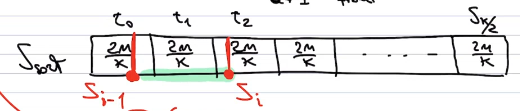
\includegraphics[scale=0.75]{4.png}
\end{center}
This means that the $a$ samples are distributed between $s_{i-1}$ and $s_i$: part in the end of $t_{j-1}$, part inside $t_j$ and part in the beginning of $t_{j+1}$. How many samples inside $t_j$, the block covered by $B_i$? They are surely $< a+1$, so $$P(\exists\: t_j\:|\: t_j\text{ is covered entirely by some }B_i) \leq P(\exists\:t_j\:|\:t_j\text{ contains less than }a+1\text{ samples})$$
We now apply the \textbf{union bound}: the probability of existence is upper bounded by the number of possibilities times the probability of one of the events. $$P(\exists\:t_j\:|\:t_j\text{ contains less than }a+1\text{ samples}) \leq \frac{k}{2}\cdot P(t_1\text{ contains less than }a+1\text{ samples})$$
We need to estimate the latter, how many samples will go to $t_1$. $$P(\text{sample occurs in }t_1) = \frac{|t_1|}{n}= \frac{\frac{2n}{k}}{n} = \frac{2}{k}$$
and the average number of samples in $t_1$, given $X_i = 1\text{ if the }i\text{th item is in }t_1$
$$X = \text{\# of samples in }t_1 = \sum_{i = 1}^{(a+1)k - 1} X_i$$
$$E[X] = E\left[\sum_i X_i\right] = \sum_{i = 1}^{(a+1)k - 1} E[X_1] = ((a+1)k - 1)\frac{2}{k} \geq 2(a+1) - 1$$ because $k \geq 2$ and $2(a+1) - 1 \geq \frac{3}{2}(a+1)$
$$E[X]\geq \frac{3}{2}(a+1) \Leftrightarrow a+1 \leq \frac{2}{3}E[X] = \left(1-\frac{1}{3}\right)E[X]$$
$P(t_1$ contains $< a+1$ sample$) = P(X < a+1)$ and we use the \textbf{Chernov Bound}: $$P(X < (1-\delta)E[X]) \leq e^{-\frac{\delta^2}{2}E[X]}$$
$$P(X<a+1)\leq P\left(X<\left(1-\frac{1}{3}\right)E[X]\right) \leq e^{-\frac{1}{18}E[X]} \leq e^{-\frac{1}{18}\cdot\frac{3}{2}(a+1)} = e^{-\frac{1}{12}(a+1)}$$
Given that $(a+1)=12\ln k$ this becomes $$e^{-\frac{1}{12}(12\ln k)} = e^{-\ln k} = \frac{1}{k}$$ $$P(t_1\text{ contains }< a+1\text{ samples}) \leq \frac{1}{k}$$
$$P\left(\exists\: B_i\:|\:|B_i|>\frac{4n}{k}\right)\leq \frac{k}{2}\cdot\frac{1}{k} = \frac{1}{2}$$
\section{Random Sampling}
I have $S[1,n] = [i_1,\ldots,i_n]$ and I want to extract $m \leq n$ elements from S randomly \textbf{with uniform probability} meaning that $P(\text{extracting }i_j)\frac{1}{n}$.\\
\texttt{rand(a, b)} extracts a random number from $[a,b]$. We consider two main scenarios: $n$ known and $n$ unknown.
\paragraph{Disk model} The sequence is of $n$ elements stored in a read-only file: $n$ is known.\\
$S = [1, n]$, build $S'$ copy of $S$. With $s =$ the number of currently sampled items (starting from $0$), we take\\\texttt{rand(1, n-s)} and swap that item with the $n$th item. Repeat the process with $n-1$, having sampled $s=1$ items.\\
We sample exactly $m$ items (repeat the process $m$ times) but we copy the entire array so we use a lot of space. We also jump a lot in the $S'$ array, so a lot of I/Os. Even though we do $m$ swaps, so low time complexity, the bottleneck are the I/Os. But if $S$ contains non-atomic items, like strings, I don't need to copy the entire objects but I can just copy the pointers: $|S'| = \#$ items, not total length.\\\\
We want to avoid the I/Os, for example by using just the indexes of the items: choose the index to sample, sort them and access the original untouched $S$ just jumping in the wanted indexes.\\
We keep a dictionary $D$ initialized as $D=\emptyset$. While $|D|<m$, we pick $p =$ \texttt{rand(1, n)} and if $p\not\in D$ we insert $D = D \cup \{p\}$. We basically pick $m$ random indexes, then we sort $D$ and extract the corresponding items from $S$.\\
As for the efficiency, we have to see how many times we pick a $p$ already in $D$ $$P(p\in D) = \frac{|D|}{n} \leq \frac{m}{n}$$ We can reason that $m\leq \frac{n}{2}$: if $m > \frac{n}{2}$ I can invert the problem and put in $D$ the items that I \textbf{don't} want to sample. With $m\leq \frac{n}{2}$ we have $$P(p\in D) \leq \frac{\frac{n}{2}}{n} = \frac{1}{2}$$ On average we pick two $p$ and one of them will go in $D$.\\\\
Another solution is to extract $m$ numbers in $[1, n]$: if they are all distinct, we sort and pick those indexes, otherwise we repeat from the start. To see if they are all distinct, I sort and if I have repetitions then two continuous items are the same.\\
It's not useful in practice: the probability of being successful is the same as the probability of having $m$ distinct items among $n$, or the birthday paradox.
\paragraph{Streaming model}
A fourth solution with $n$ known but in the streaming model: I have a continuous stream of items and I want to decide immediately for each item whether to take it or not.\\
$P(\text{sample }i_j) = \frac{m - s}{n - j + 1}$ with $s$ being the number of the currently sampled items. If $P \leq \frac{m - s}{n - j + 1}$ then $i_j$ is picked.\\
An example:
\begin{list}{}{}
	\item $M = 2$, $n = 8$ items which are $[a, b, c, d, e, f, g, h]$
	\item $P = [.5, .5, 0, .5, 1, 0, 1, 1] \leftarrow$ \texttt{rand[0,1]}
	\item $s = 0, j = 1$ extracts a probability ($.5$) and compare $P$ against the $P($sample $i_j)$\\
	$P = .5 \leq \frac{2 - 0}{8 - 1 + 1} = \frac{1}{4}$, first item not picked
	\item $s = 0, j = 2, P = .5 \leq \frac{2 - 0}{8 - 2 + 1} = \frac{2}{7}$, not picked
	\item $s = 0, j = 3, P = 0 \leq \frac{2 - 0}{8 - 3 + 1} = \frac{1}{3}$, $c$ is picked
	\item $s = 1, j = 4, P = .5 \leq \frac{2 - 1}{8 - 4 + 1} = \frac{1}{5}$, not picked
	\item $s = 1, j = 5, P = 1 \leq \frac{2 - 1}{8 - 5 + 1} = \frac{1}{4}$, not picked
	\item $s = 1, j = 6, P = 0 \leq \frac{2 - 1}{8 - 6 + 1} = \frac{1}{3}$, $f$ is picked
	\item $M = 2$ and we've picked two items, the end
\end{list}
At $m=1$ surely $s=0$ $$P(\text{pick }i_j) = P(\text{not picking }i_1,\ldots, i_{j-1})\cdot P(\text{pick }i_j) = $$\begin{list}{}{}
	\item $P(\text{not picking }i_1,\ldots, i_{j-1}) = 1 - \sum_{k=1}^{j-1} P(\text{pick }i_k) = 1- \frac{j-1}{n}$ because every $j_k$ is picked with probability $\frac{1}{n}$ independently from the others.
	\item $P(\text{pick }i_j) = \frac{m - s}{n - j + 1} = \frac{1}{n-j+1}$ given by the algorithm
\end{list}
$$ = \frac{\cancel{n-j+1}}{n}\cdot\frac{1}{\cancel{n-j+1}} = \frac{1}{n}$$ So we have a uniform probability when picking $m=1$ items.\\
What is $P(\text{pick }i_j\text{ given that we have to pick other }s\text{ elements})$? At $j$ we are left with $n-j+1$ items to consider and we have to pick yet $m-s$ items. So we can choose $m-s$ items among $n-j+1$ items: $\left(\begin{array}{c}
n-j+1\\m-s
\end{array}\right)$ possibilities. The positive event is when $i_j$ has been picked, so $m-s-1$ other samples to choose other than $i_j$ among the $n-j$ remaining without $i_j$: $\left(\begin{array}{c}
n-j\\m-s-1
\end{array}\right)$. Solving the ratio we get $\frac{\displaystyle m-s}{\displaystyle n-j+1}$.
\paragraph{Reservoir Sampling} Still streaming model but $n$ is unknown. Reservoir initialized with first $M$ items, $R = [a, b, c]$. For each value in $S$ we pick $p=$\texttt{rand(1, j)} so the number assigned is always $\geq$ than the current position.\\
An example with $M = 3$
\begin{center}
	\begin{tabular}{r c c c c c c c c c c c}
	$S=[$ & a&b&c&d&e&f&g&h&i&\ldots&]\\
	\texttt{rand(1, j)=} & \_&\_&\_&2&4&1&2&3&1
	\end{tabular}
\end{center}
\begin{list}{}{}
	\item We consider the item $d$, extracts position $2 < 3 = M$ and substitutes $b$ in the reservoir, $R = [a, d, c]$
	\item $e$, position $4 > 3$ nothing changes
	\item $f$, position $1 < 3$ and substitutes $a$, $R =  [f, d, c]$
	\item $g$, $R = [f, g, c]$
	\item $h$, $R = [f, g, h]$
	\item $i$, $R = [i, g, h]$
\end{list}
So the probability that $i_j$ is stored in $R$ is $\frac{m}{j}$: the probability is $\in [1,j]$ and $m$ are the values needed to pick it.\\
$P(i_j\in R$ after $n$ steps$)$ must be $\frac{1}{n}$. Since when we discard an item it's discarded forever, in order for $i_j$ to be in $R$ at the $n$th step it had to be in the reservoir at the $n-1$th step. At the $n$th step, in order for $i_j$ to stay in $R$ either two cases need to happen: $i_n$ is not taken (therefore $R$ doesn't change) or $i_n$ is taken and goes in a position different from the one of $i_j$.
\pagebreak
$$P(i_j\in R\text{ after }n\text{ steps})= P(i_j\in R\text{ after }n-1\text{ steps})\cdot( P(i_n\text{ is not taken})+ P(i_n\text{ is taken})\cdot P(i_j\text{ is not kicked out}))=$$
\begin{list}{}{}
	\item $P(i_j\in R\text{ after }n-1\text{ steps}) = \frac{\displaystyle m}{\displaystyle n-1}$
	\item $P(i_n\text{ is not taken}) = 1-\frac{\displaystyle m}{\displaystyle n}$
	\item $P(i_n\text{ is taken}) = \frac{\displaystyle m}{\displaystyle n}$
	\item $P(i_j\text{ is not kicked out}) = \frac{\displaystyle m-1}{\displaystyle m}$ ($m$ positions for $i_n$ minus the one occupied by $i_j$)
\end{list}
$$=\frac{m}{n-1} \left( \left( 1-\frac{m}{n}\right) + \frac{\cancel{m}}{n}\cdot\frac{m-1}{\cancel{m}}\right) = \frac{m}{n-1}\left(\frac{n - \cancel{m}}{n} + \frac{\cancel{m} - 1}{n}\right) =\frac{m}{\cancel{n- 1}}\cdot\frac{\cancel{n - 1}}{n}= \frac{m}{n}$$
The base case is $n=m$, the starting point, and we have $P(i_n$ stored in $R) = \frac{m}{j} = \frac{m}{m} = 1$, guaranteed by the initialization.
\paragraph{Disk Striping} $D > 1$. Several disks, the pages of the disks are linked: first page of all $D$ disks are a single page. So it's considered as a single disk with $B' = D\cdot B$\\
In sorting, the bound is $O(\frac{n}{DB}\cdot\log_{\frac{M}{DB}} \frac{n}{M})$ over $D$ disks with disk striping. The lower bound is $\Omega(\frac{n}{DB}\cdot\log_{\frac{M}{B}} \frac{n}{M})$
$$\frac{\frac{n}{DB}\cdot\log_{\frac{M}{DB}} \frac{n}{M}}{\frac{n}{DB}\cdot\log_{\frac{M}{B}} \frac{n}{M}} \geq 1$$
$$\frac{\log_2 \frac{n}{M}}{\log_2 \frac{M}{DB}}\cdot \frac{\log_2 \frac{M}{B}}{\log_2 \frac{n}{M}}$$
$$\frac{\log_2 \frac{M}{B}}{\log_2 \frac{M}{B} - \log_2 D}$$
$$\frac{1}{1 - \frac{\log_2 D}{\log_2 \frac{M}{B}}}$$
$$\frac{1}{1 - \log_{\frac{M}{B}} D}$$
$\frac{\displaystyle M}{\displaystyle B}$ tipically thousands, $D$ at most 10-20, so $\log_{\frac{M}{B}} D < 1$. $M\to\infty \Rightarrow 1$ optimal. $M\to DB \Rightarrow \infty$, very very slow.
\section{Randomized data structures}
\subsection{Treap} From binary search TREe and hEAP.\\
Every node is divided in two parts: one is the key and the other is the priority. A treap is a binary search tree according to the key and a heap according to the priority. To distinguish, letters for the key and numbers for the priority and we consider a maximum heap.\\
Taken a node, in the left subtree the keys will be smaller than the root, the right will have larger keys. The left and right tree, being a maximum heap, have smaller priorities: so the root has the maximum priority.\\
Let's consider the following Treap:
\begin{center}
\Tree [.M,9 [.H,8 [.G,3 ] [.I,6 ] ] [.T,7 [.R,5 [.O,4 ] ] ] ]
\end{center}
The keys are given, but the priorities are extracted at random. So the idea is that whenever you have a key to insert, you draw at random a number that you associate to the key as a priority. The randomized priorities makes the Treap balanced on average.
\paragraph{3-Sided Range Query} We build a graph with the keys on the $x$ axis and the priorities on the $y$ axis.
\begin{center}
	\begin{tikzpicture}
		\begin{axis}[axis lines=middle,axis equal,grid=none,xticklabels={G,H,I,L,M,N,O,P,Q,R,S,T},xtick={1,2,3,4,5,6,7,8,9,10,11,12}]
		\addplot[mark=*] coordinates{(5,9)};
		\addplot[mark=*] coordinates{(2,8)};
		\addplot[mark=*] coordinates{(1,3)};
		\addplot[mark=*] coordinates{(3,6)};
		\addplot[mark=*] coordinates{(12,7)};
		\addplot[mark=*] coordinates{(10,5)};
		\addplot[mark=*] coordinates{(7,4)};
		\end{axis}
	\end{tikzpicture}
\end{center}
A typical query is indicated by $[a,b] \times [c,\infty]$, with $[a,b]$ on the $x$ axis and $[c,\infty]$ on the $y$ axis. The $x$ axis so is bounded, for example by $[L, P]$, and for example $[5, \infty]$ makes the priority of the query we are looking for start from $5$ upward. So the example becomes:
\begin{center}
	\begin{tikzpicture}
		\begin{axis}[axis lines=middle,axis equal,grid=none,xticklabels={G,H,I,L,M,N,O,P,Q,R,S,T},xtick={1,2,3,4,5,6,7,8,9,10,11,12}]
		\addplot[red, mark=*] coordinates{(5,9)};
		\addplot[mark=*] coordinates{(2,8)};
		\addplot[mark=*] coordinates{(1,3)};
		\addplot[mark=*] coordinates{(3,6)};
		\addplot[mark=*] coordinates{(12,7)};
		\addplot[mark=*] coordinates{(10,5)};
		\addplot[mark=*] coordinates{(7,4)};
		\addplot +[blue, mark=none] coordinates {(4, 0) (4, 11)};
		\addplot +[blue, mark=none] coordinates {(8, 0) (8, 11)};
		\addplot +[blue, mark=none] coordinates {(0, 5) (13, 5)};
		\end{axis}
	\end{tikzpicture}
\end{center}
The data structure should return the $M,9$ point, marked in the plot, because it's the only point in the set that resides in the query.\\
The root has highest priority, so in the plane is the topmost point. The left subtree is the subplot on the lower-left side of the root point, and the right subtree is the lower-right subplot
\begin{center}
	\begin{tikzpicture}
		\begin{axis}[axis lines=middle,axis equal,grid=none,xticklabels={G,H,I,L,M,N,O,P,Q,R,S,T},xtick={1,2,3,4,5,6,7,8,9,10,11,12}]
		\addplot[mark=*] coordinates{(5,9)};
		\addplot[mark=*] coordinates{(2,8)};
		\addplot[mark=*] coordinates{(1,3)};
		\addplot[mark=*] coordinates{(3,6)};
		\addplot[mark=*] coordinates{(12,7)};
		\addplot[mark=*] coordinates{(10,5)};
		\addplot[mark=*] coordinates{(7,4)};
		\addplot +[black, mark=none] coordinates {(4, 0) (4, 11)};
		\addplot +[black, mark=none] coordinates {(8, 0) (8, 11)};
		\addplot +[black, mark=none] coordinates {(0, 5) (13, 5)};
		\addplot +[blue, mark=none] coordinates {(5, 0) (5, 11)};
		\addplot +[blue, mark=none] coordinates {(0, 9) (13, 9)};
		\end{axis}
	\end{tikzpicture}
\end{center}
Then you recurse: find the root in the left subtree (topmost point) and create two other subplots \textbf{but limited to this subplot}. Example in the left subplot:
\begin{center}
	\begin{tikzpicture}
		\begin{axis}[axis lines=middle,axis equal,grid=none,xticklabels={G,H,I,L,M,N,O,P,Q,R,S,T},xtick={1,2,3,4,5,6,7,8,9,10,11,12}]
		\addplot[mark=*] coordinates{(5,9)};
		\addplot[mark=*] coordinates{(2,8)};
		\addplot[mark=*] coordinates{(1,3)};
		\addplot[mark=*] coordinates{(3,6)};
		\addplot[mark=*] coordinates{(12,7)};
		\addplot[mark=*] coordinates{(10,5)};
		\addplot[mark=*] coordinates{(7,4)};
		\addplot +[black, mark=none] coordinates {(4, 0) (4, 11)};
		\addplot +[black, mark=none] coordinates {(8, 0) (8, 11)};
		\addplot +[black, mark=none] coordinates {(0, 5) (13, 5)};
		\addplot +[black, mark=none] coordinates {(5, 0) (5, 11)};
		\addplot +[black, mark=none] coordinates {(0, 9) (13, 9)};
		\addplot +[blue, mark=none] coordinates {(2, 0) (2, 9)};
		\addplot +[blue, mark=none] coordinates {(0, 8) (5, 8)};
		\end{axis}
	\end{tikzpicture}
\end{center}
This was the approach in computational geometry, but the data structures are exactly the same.\\
So \textbf{start from the root} and \textbf{check if it's in the} 3-sided range \textbf{query}. In this case \textbf{is in the query, so we return it as a result and we go both left and right}: this corresponds to going to the left and right subtree in the treap. In the left subtree, we recur: is the root in the query? In this case, no but the height (priority) is still larger than the "bottom", the $c$ value, so we go down but we don't go to the left subtree, which it's totally discarded, \textbf{we go to the right subtree}. If we went to the right subtree from the topmost root, that point it's still not in the query and still above $c$. Being in the right subtree, this time we go its left subtree and discard its right subtree. Basically \textbf{we move toward the $b$ value when we are on the right and toward $a$ when we are on the left}.\\
When we arrive in a node below the $c$ value we know that, being a maximum heap, everything below that has a lower priority so we can drop everything.
\subparagraph{Complexity} We want to evaluate how much "wasted work" is done, as in \textbf{how many nodes outside the query we evaluate}. The number of points is equal to the depth of the tree, because we go only left or only right and always down one level, so given $h$ height of the treap, the number of extra points we check is $O(h)$, one node extra per level at most. Inside the query we evaluate both left and right subtrees, but those are all "good" points that go into the result, so it's no wasted work. The particular case happens when we check the node just above $c$ and in the query zone: for each of those nodes we check both subtrees, all of them will have priority $< c$ and will be cut out, but we check them. Those subtrees are at most twice the number of points of the result, the number of occurrencies. So the total number of work wasted is $h$ to the left, $h$ to the right plus the occurrencies for the subtrees below $c$. The total cost then is $O(h + \text{occurrencies})$. Of course the occurrencies cannot be avoided, as we have to list them.\\
The extra cost, $h$, is typically $\log n$ if the treap is balanced with $n$ being the number of points.
\paragraph{Rotation} Considering 
\begin{center}
\Tree [.$y$ [.$x$ [.\triangled{$\alpha$} ] [.\triangled{$\beta$} ] ] [.\triangled{$\gamma$} ] ]
\end{center}
In the right rotation, node $x$ goes up and node $y$ goes down. $\alpha$ was the left subtree of $x$ and remains that, same for $\gamma$ that remains the right subtree of node $y$. $\beta$ cannot remain linked to $x$ , so $\beta$ will be relocated as the left subtree of $y$.
\begin{center}
\Tree [.$x$ [.\triangled{$\alpha$} ] [.$y$ [.\triangled{$\beta$} ] [.\triangled{$\gamma$} ] ] ]
\end{center}
We claim that this relocation still guarantees the balancing of the treap. We can pick a node $k$ inside $\beta$
$$\text{key}(x) \leq \text{key}(k) \leq \text{key}(y)$$
because it's in the right subtree of $x$ (therefore, larger key) but it's inside the left subtree of $y$ (therefore, smaller key). When we go to $\beta$ as left subtree of $y$ after the rotation, so $y$ inside the right subtree of $x$, we have that a node $k$ inside $\beta$ satisfies the same condition: it's still in the left subtree of $y$, therefore has smaller key, and still in the right subtree of $x$, therefore greater key. So the relocation preserves the conditions.\\
It's constant time, $O(1)$, because we change a constant number of pointers.
\paragraph{Search($k$)} It's just the search in the binary search tree. Based on the searched key, we go on the left if it's smaller and on the right if it's larger, so priority is not needed. Cost is $O(h)$ with $h$ being the height of the tree.
\paragraph{Insertion($k, p$)} For example inserting $(S,6)$. We start by searching for the position of $S$ in the tree. Bigger than M, smaller than T, larger than R and empty so that's the spot.
\begin{center}
\Tree [.M,9 [.H,8 [.G,3 ] [.I,6 ] ] [.T,7 [.R,5 [.O,4 ] [.S,6 ] ] ] ]
\end{center}
It's still a binary search tree but it's not an heap because the priority 6 doesn't satisfy the condition. So like in the heap we have to check the balance: S,6 needs to go up but we have to preserve the heap property so we apply a rotation, in this case a left rotation because it's the right child.
\begin{center}
\Tree [.M,9 [.H,8 [.G,3 ] [.I,6 ] ] [.T,7 [.S,6 [.R,5 [.O,4 ] ] ] ] ]
\end{center}
So it's a search plus rotation to reestablish the heap property. The rotation is constant, but in the worst case there are $h$ rotations. So the cost is again $O(h)$.
\paragraph{Delete($k$)} The deletion is trivial when we delete leafs. But for example let's remove T: we can make it a leaf by setting the priority to $-\infty$. So deletion is just: search for $k$, set the priority to $-\infty$ and then apply rotations to reestablish the heap property, then delete. Again, $O(h)$.\\
Of course in this particular case T has just one child, so we could remove it and link S as right subtree of M, but the procedure above handles every possible case.
\paragraph{Merge$(T_1,T_2)$} $\forall\:x\in T_1$ and $\forall\:y\in T_2$ we have $\text{key}(x)<\text{key}(y)$.\\
We create a root with a logical key between the maximum key of $T_1$ and the minimum key of $T_2$ and $-\infty$ as the priority. The problem is the priority: it's a binary search tree (both $T_i$ are, and the chosen key mantains that condition) but the $-\infty$ priority breaks the heap condition. But we know we can apply rotations to reestablish the condition: the root goes down until it reaches the leaf level, where it can be dropped. When this happens, the rest of the "stuff" will be a treap. So again it's $O(h)$: creating the node it's constant and the rotations are $O(h)$.\\
The reverse operation is the split.
\paragraph{Split($k, T$)} Splitting $T$ according to the key $k$ means creating a treap $T_{<k}$ with keys $< k$ and another treap $T_{>k}$ with keys $> k$. This assuming $k\not\in T$. The split is trivial when the key is the root, so I need to put myself in a situation where $k$ occupies the root. So we first insert $k,\infty$, so that it goes to the root. At insertion, $k,\infty$ will be a leaf, so we rotate to reestablish the heap priority, arriving in a situation where we have $k,\infty$ as root with a left and a right subtree. The left subtree will be $T_{<k}$ and the right subtree will be $T_{>k}$ so the we delete the root. This costs $O(h)$ for insertion, $O(h)$ for rotations and constant for deleting the root, overall $O(h)$.
\paragraph{On average, a treap is balanced} By drawing the priorities at random, the average treap is balanced. $h$ height of the treap, it's $n$ if it's just a path or $\log n$ if it's balanced, but $h = O(\log n)$ on average. Let's prove it.\\
Let's create an indicator variable $$A_k^i = \left\{ \begin{array}{c l}
1&\text{if }x_i\text{ is a proper ancestor of }x_k\\
0&\text{otherwise}
\end{array}\right.$$
$$\text{depth}(x_k) = \sum_{i=1}^k A_k^i = \text{proper ancestors of }x_k$$ $$E[\text{depth}(x_k)] = E\left[\sum_{i=1}^k A_k^i\right] = \sum_{i=1}^k E[A_k^i]=$$ and the expected value of a indicator variable is the probability of it being 1 so $$= \sum_{i=1}^k P(A_k^i = 1)$$ which is the probability of $x_i$ being on the path to $x_k$.\\
We consider $X(i,k)=\{x_i,x_{i+1},\ldots,x_{k-1}, x_k\}$ sorted, and $x_i < x_k$ or vice versa, is totally symmetric.\\
So $\text{priority}(x_i) > \text{priority}(x_k)$\\
\textbf{Theorem}: $\forall\: i \neq k$ we have that $x_i$ is a proper ancestor of $x_k \Leftrightarrow \text{priority}(x_i)$ is the largest in $X(i,k) = \{x_i,\ldots,x_k\}$. In the minimum heap the priority would be the smallest.\\
Various cases:
\begin{enumerate}
	\item $x_r$ with largest priority and $x_r,\ldots, x_i,\ldots, x_k$, $\Rightarrow x_r$ becomes the root of the treap and the $x_i,\ldots, x_k$ goes to the right subtree. So we consider the subtree.\\
	Same for $x_r$ with largest priority and $x_i,\ldots, x_k,\ldots, x_r$. $x_r$ still root and $x_i,\ldots,x_k$ in the left subtree.\\
	So this case is not significative, we restrict the attention to the $X(i,k)$ set.
	\item $x_i$ has the largest priority $\Rightarrow x_i$ is the root of the treap and $x_k$ goes to the right, so $x_i$ \textbf{is an ancestor} of $x_k$.
	\item $x_j$ has the largest priority, where $x_j\neq x_i$ and $x_j \in X(i,k)$, it's one of the items $\Rightarrow x_j$ to the root, $x_i$ to the left and $x_k$ to the right. So $x_i$ \textbf{is not an ancestor} of $x_k$.
\end{enumerate}
$$P(x_i\text{ ancestor of }x_k) = P(x_i\text{ has the largest priority of }X(i,k))=$$ Since the priorities are picked at random $$= \frac{1}{|X(i,k)|} = \left\{\begin{array}{c c}
\frac{1}{\displaystyle k - i + 1} & \text{if }i<k\\
\frac{1}{\displaystyle i - k + 1} & \text{if }i>k
\end{array}\right.$$
Not $\frac{1}{n}$ because we consider only the subset of $X(i,k)$
$$\sum_{i=1, i\neq k}^n \frac{1}{|X(i,k)|} =  \underset{\simeq \log_2k}{\underbrace{\sum_{i = 1}^{k-1}\frac{1}{k-i + 1}}} + \underset{\simeq \log_s(n-k+1)}{\underbrace{\sum_{i = k+1}^n \frac{1}{i - k + 1}}}$$ the first goes like $\log_2 k$ (because it goes like $\frac{1}{k} + \frac{1}{k-1} + \ldots + \frac{1}{2}$) and the second goes like $\log_2 (n - k + 1)$ (because it goes like $\frac{1}{2} + \frac{1}{3} + \ldots + \frac{1}{n-k+1}$).\\
With $k < n$ we have that both quantities are $\leq \log_2 n$, so
$$P(x_i\text{ ancestor of }x_k) = O(\log n)$$
If the keys are inserted in random order, so that priority = order of insertion, then the average depth is $O(\log n)$.
\pagebreak
\subsection{Skip lists} We have a list of items $L_0 = -\infty \rightarrow 3 \rightarrow 6 \rightarrow 7 \rightarrow 10 \rightarrow 15 \rightarrow 16 \rightarrow +\infty$ with $\pm\infty$ logical marks. The search in lists is very bad, the idea is to create levels of lists. List of level $L_1 = -\infty \ldots +\infty$ with vertical pointers.
\begin{center}
	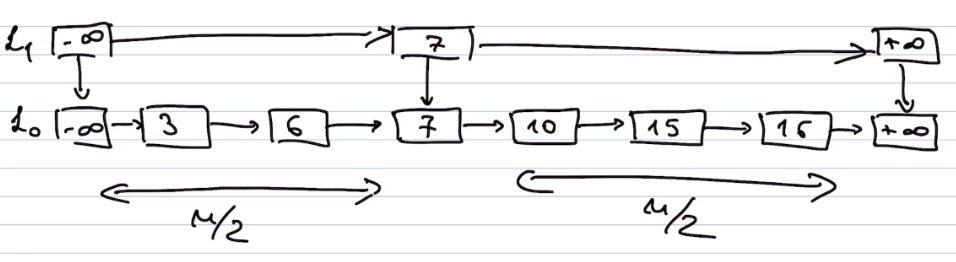
\includegraphics[scale=0.5]{5.png}
\end{center}
We can promote $k$ items to $L_1$, $k + \frac{n}{k} \Rightarrow k = \sqrt{n}$. The item are promoted randomly. For every item in $L_0$, it is promoted with probability = $\frac{1}{2}$ (e.g. coin toss, tails promotes heads doesn't), promoting $\frac{n}{2}$ items on average. This can be done for more levels.
\begin{center}
	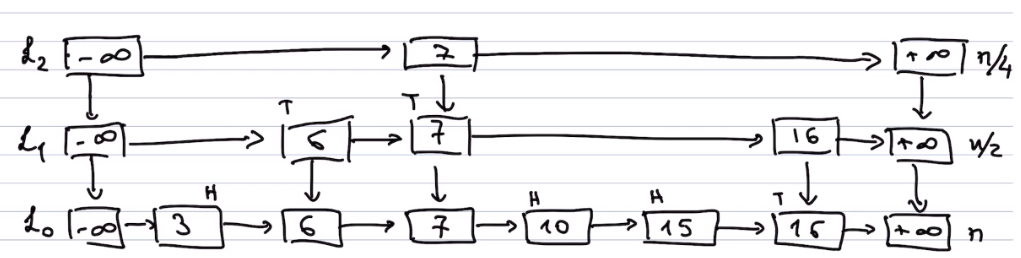
\includegraphics[scale=0.5]{6.png}
\end{center}
\paragraph{Search} We search for the topmost list, compare and go to the correct portion in the list below. At every step I scan the list if the element I'm looking for is larger and go to the list below if it's smaller.
\paragraph{Deletion} The deletion removes the column of items, in every list that item appears. In the worst case we reconstruct $\log n$ lists.
\paragraph{Insertion} First you find the position in $L_0$ (search, beginning from the topmost list), you insert and then toss the coin to insert in the upper list. To identify the left/right part in the upper list, we look for the latest item for every level that I have seen before going down during the search phase, in a sense that's the frontier to the item to be inserted.
\begin{center}
	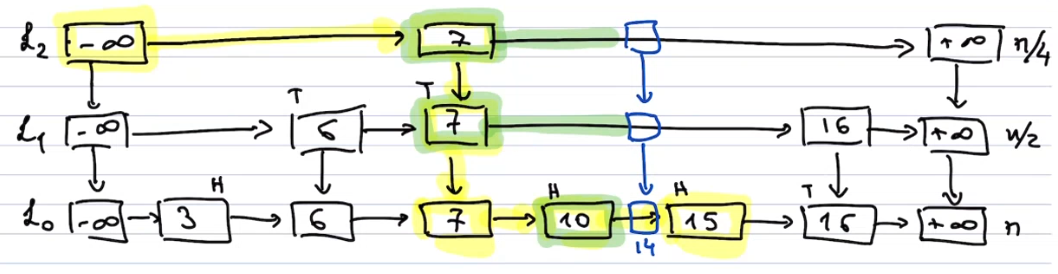
\includegraphics[scale=0.5]{9.png}
\end{center}
So keep track of the items that go down and adjust the pointers of those items.
\paragraph{Height of the skip list} $L =$ \# of levels of the skip list on $n$ items $= \max_k L(k)$ with $L(k) =$ level of the $k$th item. So the height of the skip list, the levels of the skip list, is the maximum level among the items.\\
$P(L(k) \geq l) = $ the probability of extracting $l$ tails (independent coin tosses) $= \left(\frac{1}{2}\right)^l$.\\
$$P(L \geq l) = P(\max_k L(k) \geq l) = P(\exists\: k\:|\: L(k) \geq l) \leq n\cdot\left(\frac{1}{2}\right)^l = \frac{n}{2^l}$$ for the union bound.
\begin{enumerate}
	\item $l \leq \log_2 n \Rightarrow \frac{n}{2^l} \geq \frac{n}{2^{\log n}} = \frac{n}{n} = 1$ so the inequality is not significant, because a probability is always $\leq 1$
	\item $l > \log_2 n \Rightarrow \frac{n}{2^l} < \frac{n}{2^{\log n}} = 1$
\end{enumerate}
$$P(L \geq c\cdot\log_2 n) \leq \frac{n}{2^{c\cdot\log_2 n}} = \frac{n}{(2^{\log n})^c} = \frac{n}{n^c} = \frac{1}{n^{c-1}}$$
In the search process we have, with high probability, \textbf{$O(\log n)$ "down steps"}. For the number of "right steps", let's observe the process in reverse: from the bottom we go to the left for as many right pointers we find, but we \textbf{go up as soon as we find a downward pointer}. How many right pointers before a vertical pointer on average? We \textbf{go left when we don't have a vertical pointer}, which means with probability $\frac{1}{2}$ because of the coin toss, so \textbf{it's a sequence of heads ended by a tail} (which means going up) so on average we have $2$ right steps. Every level is independent, so it applies to every level.\\
So $O(\log n)$ down steps and $O(\log n)$ right steps for the search process, so the total cost of search is $O(\log n)$. Insertion is a search plus a constant number of pointers change, deletion is a search plus a constant number of pointers change so everything is $\log n$.
\section{Set Intersection}
From a mathematical point of view we have $A,B\subseteq N$ and we want to compute $A \cap B$ fast. With $|A| = n, |B| = m$, in the case of unsorted sets, the comparison has complexity of $O(n\cdot m)$. We assume sorted sets, so we first sort $A$ and $B$ and then apply one of the algorithms that we'll see.
\subsection{Merge Based Intersection}
Based on the merge procedure seen in merge sort. For example $A = \underline{1},5,8,9,\ldots$ and $B = \underline{2}, 5, 9,\ldots$ with pointers on $1\in A$ and $2\in B$, the first elements. In the merge sort we do the comparison and write the minimum, advance the pointer in the corresponding list and go on. In the example we would end up with $1, 2, 5, 5, 8,\ldots$ But we want to simplify this. In this algorithm, whenever two items are compared, the minimum one is discarded and if the items are equal then it goes into the intersection.\\
It's linear in both lists, so the complexity is $O(n + m)$. This approach is optimal whenever $n$ is in the same order of $m$, or equal.
\subsection{Binary Search} Assuming $n > m$. For each element in $B$, we binary search for it in $A$. Every search takes $\log n$, so this costs $O(m\cdot\log n)$.\\
This approach is better than the previous, of $O(n + m)$ complexity, when $m\log n < n \Leftrightarrow m < \frac{n}{\log n}$. So it's better up to a very long $B$, which means that doing a continuous binary search is better than the merge based intersection.\\
This is true in theory, \textbf{in practice scanning} (the merge based intersection) \textbf{is typically very fast}.
\subsection{Mutual Partitioning} Still $n > m$. Let's say we take the first item of $B$, binary search over $A$ and find that it's between two certain values in $A$. When we pick the second item of $B$, in the binary search we start from scratch, but it's nonsensical because \textbf{the second item is larger than the previous item of $B$}, so we can \textbf{search only in the last right partition of $A$} that's left. This way we always go to the right, but if the first item is at the beginning of $A$ we don't advance very much so we try to balance the partitioning: instead of picking the first element of $B$, we pick the middle element (in position $\frac{m}{2}$).\\
That middle element will be found to occur between two elements in $A$, and this splits $A$ into:
\begin{list}{}{}
	\item $A_1$: until the left element included
	\item $A_2$: from the right element included
\end{list}
This also splits $B$ into two parts: 
\begin{list}{}{}
	\item $B_1$: the left half until the middle element excluded
	\item $B_2$: the right half from the middle element excluded
\end{list}
If that element is found in $A$, we return it (it belongs to the intersection) and we do the same process with the four halves that are left.\\
After $\log n$ steps, the binary search, we have turned $A \cap B$ into two problems: $A_1 \cap B_1$ and $A_2 \cap B_2$, over which we can recurse.\\
We have that $|B_1| = |B_2| = \frac{m}{2}$, with a $\pm 1$ in case of odd $m$. Those two partitions will be again divided, and so on. So we make $\log m$ recursive steps. The complexity is 
$$T(n, m) = \underset{\text{Binary Search}}{\underbrace{O(\log n)}}+ \underset{\text{Recursion over }A_1 \cap B_1}{\underbrace{T\left(n_1, \frac{m}{2}\right)}}+ \underset{\text{Recursion over }A_2 \cap B_2}{\underbrace{T\left(n_2, \frac{m}{2}\right)}}$$
To solve this we have to make some assumptions:
\begin{list}{}{}
	\item If the partitioning is \textbf{fully unbalanced} (the middle element of $B$ goes either all the way to the left or all the way to the right of $A$)\\
	 It's a \textbf{good case} because, although we keep all $A$ \textbf{we still drop half of $B$}. We either have $A_1 = \emptyset$ or $A_2 = \emptyset$ but still dropping $\frac{m}{2}$ elements. So in this case $n,m \rightarrow n, \frac{m}{2}\rightarrow n, \frac{m}{4}\ldots$ supposing that every step is fully unbalanced. We have all $n$, so the cost is guided by the binary search over $A$ with $|A| = n$ which we do $\log m$ times, so the total cost is $O(\log n \cdot \log m)$
	 \item If the partitioning is \textbf{fully balanced}, meaning that the item of $B$ that we search for ends up in the middle of $A$, so $|A_1| = |A_2| = \frac{n}{2}$ and $T(n, m) = O(\log n) + T(\frac{n}{2}, \frac{m}{2}) + T(\frac{n}{2}, \frac{m}{2})$ which if solved gives $T(n, m) = O(m(1 + \log\frac{n}{m}))$
\end{list}
A theorem states that if we have $s(n)$ solutions, a comparison based algorithm must execute $\Omega(\log_2 S(n))$ comparisons. In this scenario, $|B| = m$ can intersect $|A| = n$ in $\left(\begin{array}{c}
n\\m
\end{array}\right)$ ways: all the possibile ways in which we can take $m$ items out of $n$ items. Inputting this as $s(n)$ gives the $T(n, m) = O(m(1 + \log\frac{n}{m}))$ seen before.
\subsection{Doubling/Exponential/Galloping Search} Let's take $A, B$ and assumes that they intersect up until the 12, in position $a_{i_{j-1}}$ $b_{j-1}$. We have
\begin{list}{}{}
	\item $A = -- 12, 16, 19, 20, 25, 27, 30, 31, 34, 38, 40, 41, 44, 45, 47, 50, 60,\ldots$
	\item $B = -- 12, 41$
\end{list}
We compare the $41\in B$ with 16, 19, 25 and then 60 $\in A$, respectively with step $1, 2, 4, 8, 16$. So we don't go one-by-one but we jump exponentially, we go on as long as we find an element that is larger, 41. When it's smaller, with 60, we stop. We discard the elements we skip until we encounter the larger element: now we know that $41$, our element, is between this element and the previous element we compared with (34), so the longer the jump the more we discard.\\
41 is $b_j$, compared with $a_{i_{j-1} + 2^k}$ and we go ahead until $a_{i_{j-1} + 2^{k-1}} < b_j \leq a_{i_{j-1} + 2^k}$\\
When the element is found (let's say in position $a_f \leq a_{i_{j-1} + 2^k}$), the search for the next element, $b_{j+1}$ will start from $a_{f+1}$. Also we always have $a_{i_{j-1}} \leq b_{j-1} < a_{i_{j-1} +1}$.
\paragraph{Complexity} Let's see how much work is done in a repetitive way. $\Delta_j = \min\{n, 2^k\}$ because if $2^k > n$ we would jump outside the array, so $\Delta_j \leq 2^k$. Also, whenever I search for $b_j$ we find it in the element $a_{i_j}$: we can say that $$a_{i_{j-1} + 2^{k-1}} < a_{i_j} \leq a_{i_{j-1} + 2^k}$$ $$2^{k-1} < i_j - i_{j-1} \leq 2^k$$ $$2^k < 2(i_j - i_{j-1})$$ $$\Delta_j < 2(i_j - i_{j-1})$$
$$\sum_{j=1}^m \Delta_j < 2\sum_{j=1}^m (i_j - i_{j-1})$$ which is a telescopic sum: $i_1 - i_0 + i_2 - i_1 + i_3 - i_2 + \ldots + i_m - i_{m-1}$, where we can simplify all the elements except for $i_0 = 0$ and $i_m$. So we have $$\sum_{j=1}^m \Delta_j < 2 i_m$$ and $i_m$ is the position of the last element of $B$ inside $A$, which cannot be greater than $n$, so $i_m \leq n$, which means $$\sum_{j=1}^m \Delta_j \leq 2n$$ There's an overlap, but it's still proportional to $A$.\\
The algorithm does $\log_2 \Delta_j$ jumps (jumping "\textit{in powers of two}") plus the binary search inside the last portion (when we encounter the greater element): that portion is surely smaller than $\Delta_j$. So the algorithm costs $$\sum_{j=1}^m O(\log_2\Delta_j + \log_2 \Delta_j)$$ $$\sum_{j=1}^m O(\log_2\Delta_j) = O\left(\sum_{j=1}^m\log_2\Delta_j\right)$$ The Jensen inequality says that this can be upper bounded by $$O\left(m\cdot\log_2\frac{\sum\Delta_j}{m}\right) = O\left(m\cdot\log\frac{2n}{m}\right)$$ because $\Delta_j \leq 2n$\\
In reality it's exactly $O(m(1+\log\frac{n}{m}))$
\subsection{Two-level memory approach} As usual $A, B$ with $|A| = n > |B| = m$ and we partition $A$ into logical blocks of size $L$ (memory word or page size, for example). For every partition we take the first key, and we build $A'$ which consists of only those first keys elements, so $|A'| = \frac{n}{L}$. We want to find out in what blocks of $A$ we can find the elements of $B$, by exploiting $A'$: the arrays are sorted, so this is enough.\\
We merge $A'$ and $B$, and so we find in which blocks of $A$ can fall the elements of $B$, by using the keys in $A'$ as dividers in the merged $A'\cup B$ array. This merge costs $O\left(m + \frac{n}{L}\right)$.\\
This division also produces buckets in $B$, and $B_i$ will be intersected with $A_i$. How many blocks of $A_i$ will be considered at most? $m$, because $B$ has $m$ elements, so in the worst case is one element of $B$ per block of $A$. So we have $|B| + mL = m + mL = O(mL)$.\\
So the total cost is $O(mL + \frac{n}{L})$. Not optimal but very good, one of the best algorithms.
\subsection{Interpolation search} Search in a set $X \subseteq N$, which is sorted $X=\{x_1,x_2,\ldots,x_n\}$. Let's define $b = \frac{\displaystyle x_n - x_1 + 1}{\displaystyle n}$ and partition $X$ into buckets of size $b$ \textbf{of the universe}. So with $b= 3$ the bucket $B_1 = \{1,2,3\}$, $B_2 = \{4,5,6\}$\ldots
\begin{center}
	\begin{tabular}{c c c c | c c | c | c c | c c | c | c}
	X= & 1 & 2 & 3 & 8 & 9 & 17 & 19 & 20 & 28 & 30 & 32 & 36\\
	 & \multicolumn{3}{c}{$B_1$} & \multicolumn{2}{c}{$B_3$} & \multicolumn{1}{c}{$B_6$} & \multicolumn{2}{c}{$B_7$} & \multicolumn{2}{c}{$B_{10}$} & \multicolumn{1}{c}{$B_{11}$} & \multicolumn{1}{c}{$B_{12}$}
	\end{tabular}
\end{center}
For every bucket we have pointers in the index array $I = 1,3,0,0,4,5\ldots$ with the indexes of the beginning and the end of the bucket in $X$. If I want to search for $y$, given that I partitioned the universe I know already the bucket of $y$: it's $B_J$ with $J = \left\lfloor\frac{\displaystyle y-x_1}{\displaystyle b}\right\rfloor + 1$, so we do a binary search over $B_J$ looking for $y$. It costs constant, for computing $J$, plus the binary search over $B_J$ which costs $O(\log_2 b)$
\paragraph{Theorem} Time complexity is $O(\log_2 \Delta)$ where $$\Delta = \frac{\max_{2,\ldots,n} x_i - x_{i-1}}{\min_{2,\ldots,n} x_i - x_{i-1}}$$ It's the first time that a complexity depends on the distribution of the data.
\subparagraph{Proof} The maximum is surely larger than the average so $$\max_{2,\ldots,n} x_i - x_{i-1} \geq \frac{\overset{\text{Telescopic sum}}{\overbrace{\sum_{i=1}^n x_i - x_{i-1}}}}{n-1}=\frac{x_n - x_1}{n-1} \geq \frac{x_n - x_1 + 1}{n} = b$$
$B_J$ cannot contain more than $\frac{\displaystyle b}{\displaystyle \min_{2,\ldots,n} x_i - x_{i-1}}$ since every element is spaced from the next by at least $\min_{2,\ldots,n} x_i - x_{i-1}$
$$|B_J| \leq \frac{b}{\min_{2,\ldots,n} x_i - x_{i-1}} \leq \frac{\max_{2,\ldots,n} x_i - x_{i-1}}{\min_{2,\ldots,n} x_i - x_{i-1}} = \Delta$$
\pagebreak
\section{Data Compression}
\paragraph{Entropy} Of a source, assuming an alphabet $\Sigma$ of symbols (characters, or digits in the case of integers), with a probability distribution $\{p_\sigma\}$ over $\Sigma$.\\
The entropy of a source is $$H = \sum_\sigma p_\sigma\cdot\log_2 \frac{1}{p_\sigma} = H_0$$ sometimes specified as $H_0$ which means no context, every symbol is independent from the previous one.\\
We know that $H_0 \geq 0$ and $\sum_\sigma p_\sigma = 1$ because is a probability distribution.
\begin{list}{}{}
	\item $H = 0 \Leftrightarrow p_\sigma = 0\vee \log_2\frac{1}{p_\sigma} = 0 \Leftrightarrow p_\sigma = 0\vee p_\sigma = 1$\\
	Because the sum is 1, this means that if $$\exists\:\sigma'\:|\:p_{\sigma'}=1 \Rightarrow \forall\:\sigma\neq\sigma'\:\:p_\sigma = 0$$
	So entropy is $0$ when one symbol has probability 1 and the other have probability $0$
	\item An upper bound is $H \leq \log_2 |\Sigma|$. The formula of the entropy has its maximum value when all the $p_\sigma$ are equal, so $H \leq \log_2 |\Sigma| \Leftrightarrow p_\sigma = \frac{1}{|\Sigma|}$, a uniform probability: we would have $$\sum_\sigma \frac{1}{|\Sigma|}\cdot\log_2|\Sigma| = |\Sigma|\cdot\left(\frac{1}{|\Sigma|}\cdot\log_2|\Sigma|\right) = \log_2|\Sigma|$$
\end{list}
So we have found that $$\text{Highly skewed probability }0 \leq H \leq \log_2 |\Sigma|\text{ Uniform probability}$$
We also have the \textbf{Theorem of Shannon}: any prefix-code for source $\Sigma$ takes an average number of bits $\geq H$ per symbol of $\Sigma$.\\
Considering a random variable $X_\sigma$ that gets value $\log_2 \frac{1}{p_\sigma}$ with probability $p_\sigma$ $$E[X] = \sum_\sigma p_\sigma\cdot\log_2\frac{1}{p_\sigma} = H$$ so $\log_2 \frac{1}{p_\sigma}$ defines the information content of $\sigma$: the \textbf{entropy is the average information content of each symbol}.\\
This also states that the optimal encoding for a symbol $\sigma$ is a codeword of length $\log_2\left(\frac{1}{p(\sigma)}\right)$
\paragraph{Code C} Algorithm that assigns sequence of bits (codewords) to symbols $\sigma\in\Sigma$.\\
For example, if $\Sigma = \{$a, b, c$\}, C = \left[\begin{array}{l}
a\rightarrow 0\\
b\rightarrow 10\\
c\rightarrow 110
\end{array}\right.$ It's a variable length code, because every symbol is encoded with a variable number of bits, and a prefix-free code, because if I compare the codewords I notice that no codeword is prefix of another one. This is important because if we designed the code like $C = \left[\begin{array}{l}
a\rightarrow 0\\
b\rightarrow 01\\
c\rightarrow 1
\end{array}\right.$ and we receive $01$ we cannot unequivocably say if the codeword was produced by the sequence ac or by b. We want uniquely decodable codes.\\
We will focus on variable-length prefix-free codes.\\\\
Looking at $C$, can we optimize it? We could reduce c and assign it the codeword 11, but we cannot encode b with just 1  because we couldn't then get the prefix-free for c.\\
We have a golden rule: more frequent symbols get shorter codewords. We want to relate the length of the codeword to the frequence of its symbol. The \textbf{average length of a code $C$} in bits is $E[C] = \sum_\sigma p_\sigma\cdot\text{length}(\text{codeword}(\sigma))$. In the example, with $p($a$) = \frac{1}{4}, p($b$) = \frac{1}{2}, p($c$) = \frac{1}{4}$, then $E[C] = p($a$)\cdot|cw($a$)| + p($b$)\cdot|cw($b$)| + p($c$)\cdot|cw($c$)| = \frac{1}{4}\cdot 2 + \frac{1}{2}\cdot 2 + \frac{1}{4}\cdot 3 = 2$ bits\\
Is the golden rule satisfied for the $C$ in the example? No because b is the most probable symbol but is not the shortest codeword. A better code for those probabilities would be $C' = \left[\begin{array}{l}
a\rightarrow 00\\
b\rightarrow 1\\
c\rightarrow 01
\end{array}\right.$, with b being the most probable symbol having the shortest length and a and c having same length, where we would get $E[C'] = \frac{1}{4}\cdot2 + \frac{1}{2}\cdot1 + \frac{1}{4}\cdot2 = 1.5$ bits which is better (and optimal, we will prove it).\\
$\forall\:C$ prefix-free $E[C] \geq H$ (Shannon), so if we can make the length of the codeword of $\sigma$ exactly $\log_2 \frac{1}{p_\sigma}$ bits we have optimality. Formally, if $|\text{cw}(\sigma)| = \log_2\frac{1}{p_\sigma} \Rightarrow C$ is optimal. But $\log_2\frac{1}{p_\sigma}$ is a real number, which cannot be a length. For it to belong to $N$, we should have $p_\sigma = 2^{-x}$.
\subsection{Integer coding}
$\Sigma = N$, we will consider sequences of integers $S = s_1s_2\ldots s_n$ with $s_i\in N$ and possibly repetitive (one or more of $s_i$ can repeat). Sometimes we have increasing sequences, such that $s_i < s_{i+1}$: if we have a sequence like this we can transform is into a sequence built by the first element and the second element encoded as the distance from the first, the third element encoded as the distance from the original second, and so on. $$S' = 1\:3\:5\:6\:9\ldots \mapsto S = 1\:2\:2\:1\:3\ldots$$ These are called $d$-gaps, or gaps, and are used in place of the increasing sequences for the encoding. Of course we can revert $S$ to its original sequence $S'$ by making the prefix sum: a number is the sum of the previous numbers, so by summing the numbers from left to right.\\
This increasing sequences occur in search engines (page ids), databases (keys), hash tables (positions of unempty slots)\ldots\\
Also if $x\in Z$ we can encode them as integers with $2x$ if $x \geq 0$ or $-2x + 1$ if $x < 0$.
\paragraph{Fixed length code} Up to now we took the maximum $s_i^* = \max_i s_i$ and encoded each $s_i$ with $1+ \lfloor \log_2 s_i^*\rfloor$ bits, a fixed-size encoding.\\
With $m = s^*$, the fixed length code encodes $s_i$ with $1+ \lfloor \log_2 m\rfloor$ bits.\\
This is optimal when $$1+ \log_2 m = \log_2 \frac{1}{p(x)}\Leftrightarrow \log_2 2m = \log_2 \frac{1}{p(x)} \Leftrightarrow p(x) = \frac{1}{2m}$$
Which is a uniform distribution from $1$ to $m$, apart from the $2$, which is the case where the fixed-length encoding is optimal.
\paragraph{Unary code} With $x>0$
$$U(x)=\underset{x-1\text{ zeros}}{\underbrace{0\ldots0}}1\:\:\:\:\:|U(x)| = x$$
Very efficient for small $x$, but with large $x$ it's inefficient. For which distribution it's optimal? We apply what we've seen before: $$|U(x)| = x = \log \frac{1}{p(x)} \Leftrightarrow  2^x = \frac{1}{p(x)} \Leftrightarrow p(x) = 2^{-x}$$ So it's optimal for highly skewed distributions, very concentrated to small numbers.

\paragraph{$\gamma$-code} Improvement over the unary code, still for $x > 0$.
$$\gamma(x) = \underset{|\text{bin(x)}|-1\text{ zeros}}{\underbrace{0\ldots0}}\:\underset{\text{Binary repr. of }x}{\underbrace{\text{bin}(x)}}$$
For example: $\gamma(9) = 000\:1001$\\
bin$(x)$ surely starts with $1$, so to decode you read the number of zeroes until you find the first $1$ and then you know how many bits to read after that $1$\\
$$|\gamma(x)| = 2\text{bin}(x) - 1 = 2\left(\lfloor\log_2 x\rfloor + 1\right) - 1 = 2\lfloor\log_2 x\rfloor + 1\text{ bits}$$
Ignoring the floor, in order to get the optimal distribution for the $\gamma$-code we need $$|\gamma(x)| = \log_2\frac{1}{p(x)} \Leftrightarrow 2\log_2 x + 1 = \log_2\frac{1}{p(x)} \Leftrightarrow \log_2 2x^2 = \log \frac{1}{p(x)} \Leftrightarrow p(x) = \frac{1}{2x^2}$$
Which is a distribution smoother than the one optimal for the Unary code.\\
The sequence $0\underline{10}00\underline{111}\,\underline{1}0\underline{11}$ is decoded as $10\:111\:1\:11 = 2\:7\:1\:3$\\
From the CPU point of view is a bad code because of bit shifts: scan the number of bits and then read the number, and bits shifts break the pipeline of the processor.\\
Also for very large numbers we have lots of zeroes so a long decoding time.

\paragraph{$\delta$-code} Again for $x>0$, $$\delta(x) = \gamma(|\text{bin}(x)|)\text{bin}(x)$$
For example, $\delta(14) = \underset{\gamma(|\text{bin(14)}|)}{\underbrace{\gamma(4)}} \underset{\text{bin(14)}}{\underbrace{1110}} = 00\:100\:\:1110$\\
$\delta$-code is advantageous with large numbers.$$|\delta(x)| = |\gamma(|\text{bin}(x)|)| + |\text{bin}(x)| = \left(2\log_2 |\text{bin}(x)| + 1\right) \left(\log_2 x + 1\right) = 2\log_2(\log_2 x + 1) + 1 + (\log_2 x + 1)=$$
$$= 2\log_2\log_2 x + \log_2 x + 2 \Rightarrow p(x) = \frac{1}{2x(\log_2 x)^2}$$

\paragraph{Rice encoding} Depends on a parameter $k$: given $x \geq 0$ computes $$q = \left\lfloor\frac{x}{2^k}\right\rfloor$$ $$r = x - q2^k \text{ with } 0\leq r \leq 2^k$$
$$R_k(x) = U(q+1)\text{bin}(r)$$
$\text{bin}(r)$ is encoded on $k$ bits: $r$ can always be encoded in $\leq k$ bits because $r \leq 2^k$. \\
For example, given $x=13, k=2$, we have $q = 3, r = 1$, hence $R_2(13) = 0001\:01$, while with $k=3$ we have $q=1$ and $r=5$ hence $R_3(13) = 01\:101$
\subparagraph{Geometric distribution} $p$ successes and $1-p$ failures, the geometric distribution is $P($the first success is after $x$ experiments$)$. $P(1) = p, P(2) = (1-p)p,\ldots,P(x) = (1-p)^{x-1}p$.\\
Also $2^k$ is almost equal to $\frac{\ln 2}{p}$\\\\
$R_k$ is optimal for the geometric distribution.\\
The problem with Rice is the unary encoding, which is hard to process (bit by bit)

\paragraph{P for delta encoding} For a bounded set of integers, in the range of $0\leq x < 2^w$, so a $w$ bits sized word. Assuming that most of the integers are small, in the range $0\leq x < 2^b - 1$, so can be represented with $b << w$ bits. For example, $w = 32, b = 4$.\\
I can represent my sequence with two arrays of bits, the first array has every integer of $b$ bits and the second has $w$ bits integers. For every symbol, if it's small enough I represent it in the first array with $b$ bits, otherwise I'll put a special escape value in the first array and the symbol is stored in the second array with $w$ bits.

\paragraph{Variable Byte encoding} Idea is that given a variable $i$ there's a binary representation $B(i)$, for example $i = 2$, then $B(i) = 10$. We use 1 bit out of 8 to make the code prefix free. So $B(i)$ is splitted in blocks of 7 bits, $B(i) = \underline{\textit{000}1101}\:\underline{1001111}$. The most significant 7 bits become a byte of $\textbf{1}0001101$ and the other $\textbf{0}101111$. Continuation bit is one if the encoding continues and 0 if the encoding ends.\\
Wasteful because we never have the initial byte of the representation (most significal bits) can never be all zero.\\
Not used in practice, lets see how to avoid the waste of space. 1 byte: 128 values ($2^7$), with 2 bytes we have 14 bits and $2^{14}$ values and so on. Using one or two bytes we can encode $2^7 + 2^{14}$ different values. This is done as follows: suppose to have $0\leq i < 2^7 + 2^{14}$. If $i < 2^7 \Rightarrow$ one byte with continuation bit $= 0$. If $2^7 \leq i < 2^7 + 2^{14}$ I encode $i-2^7$ in two bytes. Clearly $0\leq i - 2^7 < 2^{14}$.\\
Reasoning in the same way with 3 bytes we can encode up to $2^7 + 2^{14} + 2^{21}$ different integers.
\paragraph{$(s, c)$ dense codes} Again byte oriented. $s$ stoppers and $c$ continuers.\\
We had every value with last bit $0$ was a stopper, while every value with continuation bit $1$ was a continuer. This means that the values in range $[0, 127]$ were all stoppers, and in range $[128, 255]$ are continuers.\\
We have chosen to have $s$ stoppers and $c$ continuers. We must have $s + c = 256$, so for example even $[0,50]$ stoppers and $[51, 255]$ continuers is acceptable. With one byte we necessarily have a stopper, so $s$ possible values because there are $s$ stoppers.\\
With 2 bytes, first one is a continuer and the second a stopper so total number is $cs$ possible values.\\
With three bytes, 2 continuers and the last a stopper so $c^2 s$ possible values.\\
Using up to three bytes the total number of possible values is $s + cs + c^2s = s(1 + c + c^2)$ which is a geometric progression of ratio $c$ so $=s\frac{c^3 - 1}{c-2}$.\\
In general using up to $k$ bytes we can encode $s\frac{(c^k - 1)}{c-1}$ different values.\\
Suppose we are encoding all positive integers $(\geq 0)$. Given $i$, how many bytes necessary to encode it? I have to find the value $k\:|\:s\frac{c^{k-1} - 1}{c-1}\leq i < s\frac{c^k-1}{c-1}$, cannot be encoded with $k-1$ bytes but can be encoded with $k$ bytes. Found $k$ we can conclude that $i$ will be encoded with $k$ bytes.
\subparagraph{Example} $s+c = 8$ so the combinations are $(s, c) = (4, 4)$, $(s, c) = (6, 2)$, $(s, c) = (5, 3)$. Let's use $(s,c) = (5,3)$ and define $000,001,010,011,100$ as stoppers and $101,110,111$ as continuers.\\
If I use one block, it can only consist of a stopper, so the values $0,1,2,3,4$, so $5$ values in total.\\
With 2 blocks, one continuer and one stopper, so each continuer can be paired with each stopper: $3$ continuers $\cdot 5$ stoppers is $15$ values in total. This way we encode the next integers, so the values $5,6\ldots,19$. This makes $5+15 = 20$ values encodable with $2$ $3$-bit blocks.\\\\
Supposing we have to encode $100$ with $(5,3)$ dense code. We have to find $k\:|\:s\frac{c^{k-1}-1}{c-1}\leq 100 < s\frac{c^k-1}{c-1}$ is satisfied.\begin{list}{}{}
	\item $k=2 \Leftrightarrow 5\frac{3^{2-1}-1}{3-1}\leq 100 < 5\frac{3^2-1}{3-1} \Leftrightarrow 5 \leq 100 < 20$
	\item $k=3 \Leftrightarrow 5\frac{3^{3-1}-1}{3-1}\leq 100 < 5\frac{3^3-1}{3-1} \Leftrightarrow 20 \leq 100 < 65$
	\item $k=4 \Leftrightarrow 5\frac{3^{4-1}-1}{3-1}\leq 100 < 5\frac{3^4-1}{3-1} \Leftrightarrow 65 \leq 100 < 200$
\end{list}
I need $k=4$ blocks, with 4 blocks we encode values in $[65, 200]$. 100 is the $100-65 = 35$th value encoded with $k=4$ blocks.\\
With two blocks we encode $5+15 = 20$ values, with three blocks we have another $45$ values so $65$ total values, with the fourth blocks we add $135$ more values, for a total of $200$ values.\\
Each codeword with exactly $4$ blocks ($cccs$) encodes at most $3^3\cdot 5 = 135$ values with $(5,3)$ dense encoding.
\paragraph{Interpolative Code} It requires that both the encoder and the decoder stays synchronized on what's going on.
\begin{center}
	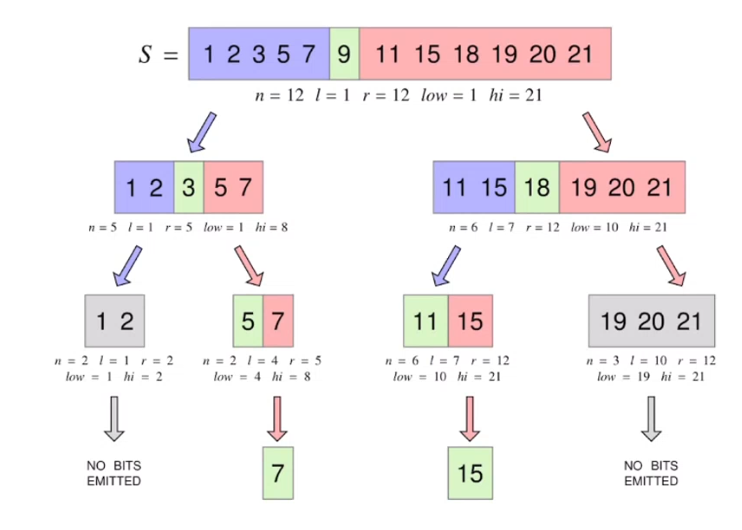
\includegraphics[scale=0.8]{11.png}
\end{center}
The first encoded item is the one in the middle of the sequence $S$ ($9$ in the example), then the interpolative encoding is recursively called on the first and second half of the sequence. Again we encode the middle item and so on.\\
The first important element is that the input sequence must be \textbf{strictly increasing}. If it's not, we can transform it by summing the item with the previous one. For example $S = 7,1,9,2,13,7,8$ become $S = 7$ (the first item as-is)$, 8$ ($1+7$), $, 17$ ($9+8$)$, 19$ ($2+17$)$, 32, 39, 47$.\\
At the beginning, the encoder writes down the indexes of the first and last item $l, r$, and the values. In the example of the image, those values are $[1,12,1,21]$. The decoder will read these values and know that there are $12$ items, the first is $1$ and the last is $21$. Then the encoder writes down the middle element (index $6$, value $9$).\\
The decoder \textbf{knows that} between position 1 and 6 there are 6 increasing numbers, so the item in position 6 will have a value of at least $6$. Also know that the last value is $21$ and $21-6 = 15$. So the middle element has a value $x$ such that $6\leq x \leq 15$.\\
The encoder writes down the difference between the actual value of the middle element, $9$, and the minimum possible value, $6$, so writes down $3$. It also knows that the difference is in the range $[0,9]$ because the maximum value is $15$, so the difference $3$ is written out with $4$ bits $\rightarrow 0011$.\\
The decoder reads $0011$, so the difference is $3$, so the actual value is $9$.\\
Now the encoder goes to the left part, whose first index is $l=1$ and last is $r=5$. We just encoded $9$, so the value in position $5$ cannot be greater than $8$. Now it writes the value in the middle position, $3$, and the value it has to encode is $3$.\\
The decoder knows that the value in position $3$ is $\geq 3$ and reasoning from the right, the value is also $\leq 6$. Four possible values, so 2 bits to encode in that range. The encoder writes $00$. Now it would proceed to the left part, but there are two elements from index $1$ to $2$ and the values are again from $1$ and not greater than $2$ because we just encoded $3$, so it's information that the decoder already knows and it starts working on the right part.\\
It needs to encode $5$, just encoded $3$ and we're on the right part, so the value must be $\geq 4$. It also knows that the last value in this part is at most $8$ because we encoded $9$, so the middle element is between $4$ and $8$, so five elements so $3$ bits where it's encoded $1$, the difference between the actual value $5$ and the minimum value $4$. We proceed, with the $7$. It's at least $6$ (we just encoded $5$) and at most $8$, so two bits.\\
It proceeds like this.\\\\
In short: we have $low, l, hi, r$, we find $m = \lfloor\frac{l+r}{2}\rfloor$ and know that $low+m-l\leq S[m]\leq hi + m - r$ so we encode $S[m] - (low + m - l)$ with $\rceil\log_2 B\rceil$ bits where $B = hi + l - r - low +1$ (or, simply, the bound size: right - left + 1).
\paragraph{Effectivness} The bits represents values in ranges, so if the ranges are small we use fewer bits. So it's efficient when values are clustered, "dense".
\paragraph{Elias Fano codes} Where we can access any value in the compressed sequence very efficiently. We have $n$ increasing values in the range $[0, u)$, $b = \lceil\log_2 u\rceil$ bits for the representation and $l = \lceil\log_2(\frac{u}{n})\rceil$, $h = b-l$. An example with $n = 8, u = 32, b = 5, l = 2, h = 3$
\begin{center}
	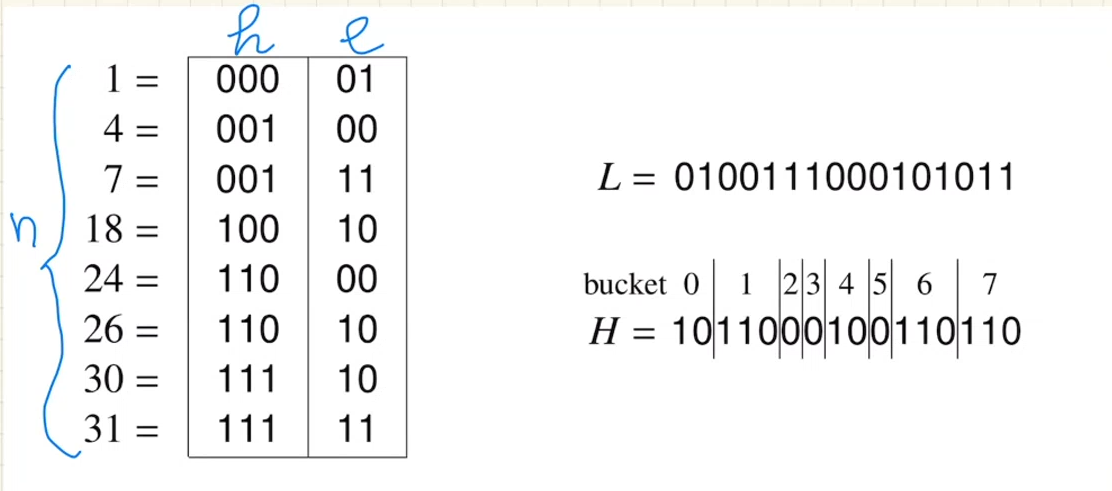
\includegraphics[scale=0.5]{12.png}
\end{center}
We work with two columns: the $l$ least significant bits and the $h$ most significant bits. The values in the $l$ column are not compressed at all, so $L$ is just the concatenation of those values. Because it has no compression, $l$ is chosen also to make $L$ small compared to the rest of the encoding.\\
The values in the $h$ column are increasing, because the values of the sequence are increasing and the most significant bits remain increasing even when removing the least significant bits. To compress $H$ the idea is the following: we know that $h=3$, so $2^h = 2^3 = 8$ possible values and maybe some of them don't appear (for example: $2,3,5$ do not appear in the example). We consider all 8 possible values and we record a unary representation of the number of items in the $h$ column with that value (in the example, only one $0$ so $10$ with as many ones as the occurrences ended by a $0$ "separator"). The values are increasing, so the one 0 is the first, the two 1 are the second and third, zero $2$, zero $3$ and then one $4$ so is the fifth.\\
\textbf{Important}: in $H$, $\#0 = 2^h$ (there are $2^h$ zeroes, separators) and $\#1 = n$ because we encode $n$ values. In $L$, \#bits $= l\cdot n$. There's a one-to-one correspondence between the 1 in $H$ and the groups of $l$ bits in $L$: the first $1$ in $H$ corresponds, in the example, to the first two bits, and that 1 indicates a group of $h$ bits with value 0, so $000\:01$.
\paragraph{Space} So we have $n$ integers $\in[1, u)$, $l=\lceil\log_2(\frac{u}{n})\rceil$, $h = b - l$ with $b=\lceil\log_2 u\rceil$\\
In $H$, we have $2^h$ zeros (buckets) and $n$ ones (because we encode $n$ values). The buckets (so, the zeros) contain each $2^l$ values, so the range $u$ is splitted over those values. This means that the buckets are $\frac{u}{2^l} = \frac{u}{2^{\lceil\log_2(\frac{u}{n})\rceil}} \leq \frac{u}{2^{\log_2(\frac{u}{n})}} = \frac{u}{\frac{u}{n}} = n$ in total. Meaning that $|H| \leq 2n$ bits.\\
In $L$ we have $n \cdot l$ bits, meaning $n\cdot\lceil\log_2(\frac{u}{n})\rceil$ bits.\\
The total space then is $\leq 2n + n\log_2(\frac{u}{n})$. We have to account the cost of the data structures for the SELECT, which is $O(n)$: the real total cost is $2n + n\log_2(\frac{u}{n}) + o(n)$
\paragraph{In general} To distinguish between $n$ numbers in a range of $[0, u)$, a code cannot use less than $\log_2\left(\begin{array}{c}
u\\n
\end{array}\right) = n\log\frac{u}{n} + o(n)$ bits.\\
So Elias-Fano is 2 bits per integer off the optimal.
\subparagraph{Decompress}
We need a data structure supporting the operation SELECT$_1$($H, i$), which returns the position of the $i$th $1$ in $H$. For example, SELECT$_1$($H, 5$) should return $11$. Of course, $0< i \leq n$\\
Assuming we want to find $S[5]$. Until now, with the other codes, we needed to decompress the whole sequence in order to get a single element. With this code we can access a single element from the compressed data. For the least significant bits we simply select the $5$th group of $l=2$ bits in $L$, which is $00$ and we get this in $O(1)$. The $5$th elements corresponds to the $5$th $1$ in $H$, and we get that position with the SELECT operation stated before (SELECT$(H,5)= 11$) but we need to know the bucket as well. To find the bucket it belongs, we simply count the number of $0$ that are before that $1$, and to count them knowing that it's the $11$th position and the $5$th $1$, we simply do $11-5=6$. So we have that the $5$th element is in the $6$th buckets and $h=3$, so the most significant bits are $110$. Putting it all together, we get $110\:00 = 24$ which is correct.\\
So ACCESS($i$) = (SELECT$_1$($i$) - $i$ in $H$) followed by ($i$-th group of $l$ bits in $L$)\\
As for NextGeq($i$), we compute $H(i)$ which are the $h$ most significative bits of $i$ and go into the first position that bucket, given by $\eta =$ SELECT$_0(H(i)) + 1$. If $H[\eta] = 1$, the bucket is empty and we scan $L$ starting from $(\eta - H(i))$th group of $l$ bits in $L$ until we find an element bigger than $i$. Its a scan of at most $2^l$ elements, so it's $O(2^l) = O(\frac{u}{n})$. If $H[\eta]=0$ we pick the first elements of the next bucket, given by Access($\eta - H(i)$).
\paragraph{Exercises}
\begin{list}{}{}
	\item \textbf{Do one level of recursion of interpolative code on} $S = 11,14,16,19,20,21,22$\\
	We begin with $l=1,r=7,min=11,max=22$, the middle element is the one in index $\lfloor\frac{7+1}{2}\rfloor = 4$ which is $19$, so it must be $(min+m-l) = 11+4-l = 14 \leq x \leq 19 = 22-7+4 = (max+m-r)$, and $19-14 = 5$ so it can be encoded with 3 bits: $19$ will be encoded with $101$.\\
	The left part is $11,12,16$ with $l=1, r = 3, min = 11, max = S[4]-1 = 18$, the middle element is $\lfloor \frac{3+1}{2}\rfloor = 2$ which is $14$ and must be $12\leq x\leq 17$, so we need $3$ bits: $14$ is encoded as $010$.\\
	The right part is $20,21,22$ with $l=5, r = 7, min = S[4]+1 = 20, max = 22$, the middle is $\lfloor \frac{7+5}{2}\rfloor = 6$ which is $21$, must be $21\leq x \leq 21$, so 0 bits. 
	\item \textbf{$\delta$-code and Rice code with $k=3$} on $S(1,6,15,18,21,24,30)$\\
	$S'=(1,5,9,3,3,3,6)$, with $\delta(x) = \gamma(|bin(x)|)\:bin(x)$ and $\gamma(y)=0\ldots0 bin(y)$ with $|bin(y)-1|$ zeroes, so:\begin{list}{}{}
		\item $\delta(1) = 11$
		\item $\delta(5) = 011101$
		\item $\delta(9) = 001001001$
		\item $\delta(3) = 01011$
		\item $\delta(6) = 011110$
	\end{list}
	As for Rice, with $k=3$ and remembering $q = \lfloor\frac{x-1}{2^k}\rfloor$ and $r = (x-1) - q2^k$ with $R_k(x) = unary(q+1)\:bin(r)$ and $U(x)=00\ldots01$ with $x-1$ zeroes, so:
	\begin{list}{}{}
		\item $R_3(1) = 1000$ with $q = \lfloor\frac{1}{2^3}\rfloor = 0$ and $r = 1-1 -0\cdot2^3 = 0$
		\item $R_3(5) = 1100$ with $q = 0$ and $r = 4$
		\item $R_3(9) = 01000$ with $q = 1$ and $r = 0$
		\item $R_3(3) = 1010$ with $q = 0$ and $r = 2$
		\item $R_3(6) = 1101$ with $q = 0$ and $r = 5$
	\end{list}
	\item \textbf{Show this $(1,3)$ codeword of $8$ on $2$-bit words}\\
	$s = 1$ stoppers $\Rightarrow \{00\}$, $c = 3$ continuers $\Rightarrow \{01,10,11\}$. So:\\
	\begin{center}
		\begin{tabular}{c l}
		\textbf{Values} & \textbf{Codewords}\\
		0 & $00\:$\\
		1 & $01\:00$\\
		2 & $10\:00$\\
		3 & $11\:00$\\
		4 & $01\:01\:00$\\
		5 & $01\:10\:00$\\
		6 & $01\:11\:00$\\
		7 & $10\:01\:00$\\
		8 & $10\:10\:00 \longleftarrow$\\
	\end{tabular}
	\end{center}
	\item \textbf{Encode $S=(1,3,4,5,9,16,23,27,28,31,40)$ with Elias-Fano and show how to answer ACCESS(4), NEXTGEQ(8) and NEXTGEQ(32)}.\\
	We have $n = 11, u = 41$, $b = \lceil\log_2 u\rceil = 6$ and $l = \lceil\log_2(\frac{u}{n})\rceil = 2$ so $h = b-l=4$. The table is \begin{center}
		\begin{tabular}{c c c}
			\textbf{Value} & \textbf{H} & \textbf{L}\\
			1 & 0000 & 01\\
			3 & 0000 & 11\\
			4 & 0001 & 00\\
			5 & 0001 & 01\\
			9 & 0010 & 01\\
			16 & 0100 & 00\\
			23 & 0101 & 11\\
			27 & 0110 & 11\\
			28 & 0111 & 00\\
			31 & 0111 & 11\\
			40 & 1010 & 00\\
		\end{tabular}
	\end{center}
	\begin{list}{}{}
		\item[$L =$] $01\:11\:00\:01\:01\:00\:11\:11\:00\:11\:00$
		\item[$H =$] $110\:110\:10\:0\:10\:10\:10\:110\:0\:0\:10\:0\:0\:0\:0\:0$
	\end{list}
	As for the operations:
	\begin{list}{}{}
		\item Access(4): $4$th group in $L$ for the least significant bits, $4$th $1$ in $H$ (SELECT$_1(4)$) for the most significant bits. We get $01$ from $L$ and the $4$th $1$ corresponds to the $2$nd bucket, which is $1$ on $h = 4$ bits $\Rightarrow 0001$, so we get $000101 = 5$
		\item NextGeq(8) = NextGeq(0010$\:$01) so we look for the starting position in $H$ for the bucket $0010 = 2$ ($\eta =$ SELECT$_0(2)+1 = 6+1 = 7$) $H[\eta] = 1$ so is a non empty bucket: we scan elements in $L$ from $\eta - H(8) = \eta - 2$ (the bucket value) $ = 5$ group and return 9.\\
		At the same time I scan $H$ and if I encounter 0 I've ended the bucket, so I return the first item of the next non-empty bucket.
		\item NextGeq(32) = NextGeq(1000$\:$00)\\
		$\eta =$ SELECT$_0(8) + 1 = 18+1 = 19$ and $H[19] = 0$ so bucket empty, we return the next element which is given by Access($\eta-H(32)$) = Access$(19-8)$ = Access$(11)$
	\end{list}
	\item \textbf{Encode $S=(11,14,16,19,20,21,22)$ with Elias-Fano and answer Access(5) and NextGeq(17)}. Reduce the Universe size by subtracting $11$ (so $5+11$ in the first and $17-11$ in the second question)
\end{list}
\section{String Sorting} Until now: atomic items. Now: sequence of symbols/characters/letters (\textbf{strings}), drawn from an alphabet $\Sigma$ with $|\Sigma| = \sigma$ symbols (often $\sigma = 256$).
We have a set of strings $S[1,n]$ with $N$ the total length and $n$ the number of strings. Also $L=\frac{N}{n}$ is the average length.\\
Usually \texttt{qsort}, comparison-based algorithm: need to specify the comparison function, meaning that \textbf{\texttt{qsort} is agnostic to the kind of objects it's sorting}, we can use it to sort strings. It costs $O(L\cdot n\cdot\log n) = O(N\cdot\log n)$ time on average (worst case if using \texttt{mergesort}, \texttt{heapsort} or other very efficient sorting algorithms). Whenever the portion between $l$ and $r$ in \texttt{qsort} is small, with atomic items we would do insertion sort because the elements would fit in few cache lines, but with strings each item is a pointer so the items are probably spread apart in memory. So we will try to improve this.\\\\
The lower bound is composed by two parts: \begin{list}{}{}
	\item I have to sort the first characters of these $n$ objects and I \textbf{cannot escape the comparison of the first objects}, so the classic lower bound $\Omega(n\cdot\log n)$
	\item The first character only is too limiting, how many characters I have to surely look at? $d_i$ is the \textbf{distinguishing prefix} and is the minimum number of characters that we have to consider in order to distinguish the string $s_i$ from the others. We do not need the rest of the characters of $s_i$ in order to distinguish it from the other strings. We can say that $d = \sum_s d_s$ is the total distinguishing prefix.\\
	So the second part of the lower bound is: \textbf{I cannot look at less than $d \sum_s d_s$ symbols}, the cumulative length of the distinguishing prefixes, $\Omega(d)$.
\end{list}
So the \textbf{lower bound for comparison-based sorting algorithms for strings} is $$\Omega(n\log n + d)$$ We can view it as time or character comparisons, and in asymptotic notation means the maximum between the two parts.
\paragraph{State of \texttt{qsort}} In the case of $n$ strings $s_i$, composed by $l$ zeroes followed by $\log n$ other characters
$$\begin{array}{r c c}
 & l & \log n\\
s_1 & 00\ldots 0 & 00\ldots 0\\
s_2 & 00\ldots 0 & 00\ldots 1\\
\vdots & \vdots & \vdots\\
s_n & 00\ldots 0 & 11\ldots 1\\
\end{array} n$$
The \texttt{qsort} is $O(L\cdot n\cdot \log n)$, $L= l+\log n$ because they have all the same length. So \texttt{qsort} is $O(l\cdot n\cdot\log n + n\cdot\log^2n)$\\
It is at least a $\log n$ factor from the lower bound, which can be very impactful due to the cache misses and the memory accesses.
\subsection{Radix sort}
\begin{list}{}{}
	\item \textbf{Most significant digit sort} (\textbf{MSD}), where we scan from the left to right
	\item \textbf{Least significant digit sort} (\textbf{LSD}), where we scan from the right to left\\
	Used in the punch cards 
\end{list}
An example: $S = \{007, 017, 042, 911, 999\}, n=5, \sigma = 10, N = 3\cdot 5 = 15$. The idea of MSD is trivial: we scan  the strings from left to right and position them according to the first character. So we have an array of size $\sigma$ and we put each item in the corresponding bucket according to the first symbol. Then we consider the second digits for every bucket, and do the same thing.
$$\begin{array}{c c c c c}
	0 & 1 & 2 & \ldots & 9\\
	\downarrow & \ & \ & \ldots & \downarrow\\
	007 & & & & 911\\
	017 & & & & 999\\
	042
\end{array}$$
$$\begin{array}{c c c c c c}
	0 & 1 & 2 & 3 & 4 & \ldots\\
	\downarrow & \downarrow & \ & \ & \downarrow & \\
	007 & 017 & & & 042 &\\
\end{array}\:\:\:\:\:\:\:\:\:\: \begin{array}{c c c c}
	0 & 1 & \ldots & 9\\
	\ & \downarrow & \ & \downarrow \\
	 & 911 & & 999\\
\end{array}$$
We go down until we have one item per bucket in each level. If we had "019", it would've gone in the second bucket of the second level, so we would have done a third level.\\
\textbf{For each element $s_i$ we create $d_i$ nodes} (arrays), \textbf{its distinguishing prefix}, but those nodes are in general shared with other strings. So $\forall$ string $s$ we create $d_s$ nodes. The total number of nodes (arrays) $\leq d = \sum_s d_s$ because some nodes are shared between strings. The arrays are of size $\sigma$, so in space terms we have $O(d\cdot \sigma)$. The sorting time is composed of: the time required to create the tree of arrays of $d\cdot\sigma$ nodes, so $O(d\cdot\sigma)$, then we have to scan the final set of strings, the last level, which is at most every possible node of the last level, another $O(d\cdot\sigma)$. So the cost is $O(d\sigma)$. This is not a comparison-based algorithm, so the lower bound stated before doesn't apply.
\paragraph{Trie} A \textbf{data structure}. It's a tree, every node is an array of $\sigma$ positions where each position have a pointer to other nodes ($\sigma$-ary tree). The \textbf{MSD algorithm builds a trie}.\\
Good and bad properties. The good is that the array is very sparsely populated, with big $\sigma$, so it's very efficient in time for searches, but it's inefficient in space ($d\cdot\sigma$).\\
Given a pattern $P[1,p]$ of $p$ characters, we can check if $P$ is in the trie or not in $O(p)$, optimal in time. With arrays it's very inefficient in space, though, because most of the arrays would be empty or almost empty especially in the leafs. We need another way of implementing an array, there are two possibilities: binary search tree or hashtable, let's see the second one.
\subparagraph{Trie with hashtables} We insert $\langle$digit, pointer$\rangle$ pairs. The idea is to create an hashtable for every node whose size is proportional to the number of distinct pairs ($\equiv\#$ edges, the pointers in the arrays). For example, an hashtable $T$ of $3$ positions where we insert the pairs $\langle 1,p_1\rangle, \langle 2,p_2\rangle, \langle \sigma,p_\sigma\rangle$ can be populated by applying the hash function to the keys and end up like $\begin{array}{c c l}
T\\
0&\rightarrow&\langle 2,p_2\rangle\\
1\\
2&\rightarrow&\langle 1,p_1,\rangle,\:\langle \sigma, p_\sigma\rangle
\end{array}$\\
So the size of the table is proportional to the number of keys, $|T|=O(\#$ keys$)$, and the cost of searching in an hashtable is $O(1)$ on average.
\subparagraph{Trie with binary search tree} In this case, the worst case time cost is $O(\log \sigma)$\\\\
In both cases we have a space complexity of $O(\#$ keys$)=O(\#$ edges$)$
\paragraph{MSD radix sort with hashtable} In every node we have and hashtable of size the number of edges but not sorted. The algorithm goes like this:
\begin{enumerate}
	\item Building the trie\\
	Search and insertion of hashtables are both $O(1)$, so we pay $1$ for every string for every level we need to go down on. So constant time $\cdot$ the number of traversed nodes, which is $d_s$ for the string $s\Rightarrow$ total time is $\sum_s O(1)\cdot d_s = O(d)$ on average time .\\
	In a binary search tree, the $O(1)$ becomes $O(\log\sigma)$ so the total cost is $O(d\cdot\log\sigma)$
	\item Sorting the hashtables to sort the edges. We can use \texttt{qsort} on the pairs, which costs $O(\#$ edges$\cdot\log_2\#$ edges$)$.\\
	Let's define $l_u$ the number of edges in the node $u$. So the total cost of sorting is $\sum_u O(l_u\cdot\log l_u)=O\left(\sum_u l_u\log l_u \right) = O\left(\sum_u l_u\log\sigma \right)$ because the number of edges in node $u$ is $\leq \sigma$ for every $u$. So we have $= O\left((\log\sigma)\cdot\sum_u l_u \right)$, the sum over all the nodes of the number of edges, which is $\leq d$. So the total cost of sorting is $O(d\cdot\log\sigma)$ in time and $O(d)$ in space.
\end{enumerate}
\paragraph{LSD radix sort} LSD scans the opposite way, from right to left, we sort every column using what's called a \textbf{stable-sort}: a sort that respects the original order, if two columns are equal. We used the counting sort, with a complexity of $O(\#$ keys$ + \sigma)$ with $|\Sigma| =$ size of the alphabet.\\
An example assuming to have the following strings \begin{list}{}{}
	\item $\begin{array}{c}
	017\\042\\665\\111\\007
	\end{array}$ first digit $\rightarrow\begin{array}{c}
	111\\042\\665\\017\\007
	\end{array}$ second digit $\rightarrow\begin{array}{c}
	007\\111\\017\\042\\665
	\end{array}$ third digit $\rightarrow\begin{array}{c}
	007\\017\\042\\111\\665
	\end{array}$
\end{list}
By respecting the order thanks to the stable sort, we get a ordered sequence. The total complexity is the $\#$ digits per string times the cost of counting sort. So $O(L\cdot(n+\sigma)) = O(Ln + L\sigma) = O(N)$ time and space.
\subparagraph{Proof of why it works} Let's focus on two strings: $x,y$, with $x<y$. Let's say they have the same prefix $\alpha$, a character $a$ for $x$ and $b$ for $y$ and then the rest of the string: $$\begin{array}{r c c c}
x = & \:\:\:\:\:\alpha\:\:\:\:\: & a & \ldots\\
y = & \:\:\:\:\:\alpha\:\:\:\:\: & b & \ldots\\
\end{array}$$
$x<y\Rightarrow a<b$, for example $x$ is "abaco" and $y$ is "abate": $\alpha =$ "aba", $a=$ c, $b=$ t.
$$\begin{array}{r c c c}
x = & \text{aba} & \text{c} & \text{o}\\
y = & \text{aba} & \text{t} & \text{e}\\
\end{array}$$
In the first phases, we compare the right part of both strings and $x$ could end up before or after $y$, it's not important. At some point, it will compare $a,b$ and since $a< b$ we will have a situation where $x$ comes before $y$. Then we compare $\alpha$, but they are equal and thanks to the stable sort the relative order between $x$ and $y$ will not change (possibly changing distance, but they will not "invert" order). This applies to every pair of strings, so the final order of strings will be a sorted order.
\subparagraph{More precise complexity} Let's assume binary strings, with $0,1$ digits and of $b$ length. We can apply the LSD radix sort to groups of $r$ bits each: $\frac{b}{r}$ groups. Each group of $r$ bits can be interpreted as a symbol, so $\sigma = 2^r$ maximum configurations of $r$ bits (from all zeroes to all ones)\\
$\frac{b}{r}$ phases each costing $n+2^r$, so the total cost is $O(\frac{b}{r}(n+2^r))$: the minimum is in $r=\log n$ and so the complexity becomes $(\frac{b}{\log n})\cdot(n+n) = O\left(\frac{n\cdot b}{\log n}\right) = O\left(\frac{N}{\log n}\right)$ time.
\subsection{Multi-key Quicksort}
The invariant is that that there is a prefix $[0, i-1]$ shared by the strings in $R$, $i$ is the character we compare and at the beginning $i=1$
\begin{lstlisting}[style=myPython]
def MKQ(R, i):
	if (|R| <= 1):
		return R
	else:
		choose a pivot string p in R
		Rless = {s in R | s[i] < p[i]}
		Req = {s in R | s[i] = p[i]}
		Rgreat = {s in R | s[i] > p[i]}
		A = MKQ(Rless, i)
		B = MKQ(Req, i+1)
		C = MKQ(Rgreat, i)
		return A + B + C
\end{lstlisting}
We have the strings, and we know that all of them share $i-1$ characters. The $i$th character of the pivot strings realizes the three-way partitioning of $R$: if the $i$th character of the string is $<$ than the $i$th character of the pivot, then that string goes into $R_<$, if it's $=$ goes into $R_=$ and if it's greater goes into $R_>$.\\
So returning the three partitions in order gives us the sorted order of the original $R$. Some considerations:
\begin{list}{}{}
	\item $|R_<|,|R_>|<|R|$ because $p$ is not in them, so their size is surely shrinking
	\item $|R_=|\leq |R|$, could be equal whenever the $i$th character of all the strings in $R$ is equal to the $i$th character of the pivot string $p$. In any case, $i$ is increased by one (also $i\leq$ maximum string length)\\
	So \textbf{the recursion is well-posed}.
\end{list}
Let's reason about complexity, taking $s\in S$ the original set, with $R=S$ at the beginning. For a generic step we have $R, i$ and there are two cases that can occur to $s$:
\begin{list}{}{}
	\item $s[i]<p[i]\rightarrow s\in R_<$ or $s[i]>p[i]\rightarrow s\in R_>$ and in both cases $|R_<|<|R|\wedge|R_>|<|R|$
	\item $s[i]=p[i]\rightarrow s\in R_=$ and $i$\texttt{++}
\end{list}
How many times we do $i$\texttt{++} on the string $s$? $i\leq d_s$ because $d_s$ is the maximum number of symbols shared with another string plus 1 (the \textbf{distinguishing} prefix), so the prefix of $s$ $s[1,d_s]$ is distinct from every other string. On average, picking a random pivot, we have that $|R_<|\simeq\frac{|R|}{2}$ and $|R_>|\simeq\frac{|R|}{2}$. This means that we have a logarithm of recursive steps, and since we're starting from $S$ we have $O(\log |S|)$ recursive steps on average.\\
For the string $s$, the numbers of recursive calls is $O(\log n + d_s)$, and $\sum_s O(\log n + d_s) = O(n\log n + d)$ average time, so it's optimal on average.
\subsection{Ternary Search Tree} It's a \textbf{ternary trie}.\\
Each node has a character and may have three outgoing edges: one is $<$, one is $=$ and one is $>$. If the node corresponds to the $i$th position and has character "c", then all the nodes in the $=$ subtree have "c" in the $i$th position, all the nodes in the $<$ subtree have characters $<$ "c" in the $i$th position and in the $>$ subtree the $i$th characters are $>$ "c". In the $<$ and $>$ subtree you still remain in the $i$th character, so the root of those subtrees still correspond the the $i$th character, while in the $=$ subtree you advance so that root corresponds to the $i+1$th character (much like the \texttt{MKQ} code before).\\
But we don't want to explode the entire string. Let's do an example with S = \{cat, abi, cast, cam, at\}:
\begin{list}{}{}
	\item We insert "cat", in an empty tree, so simply
		\begin{center}
			\Tree [.C [. ] [.cat ] [. ] ]
		\end{center}
	\item "abi" in the $<$ subtree
		\begin{center}
			\Tree [.C [.abi ] [.cat ] [. ] ]
		\end{center}
	\item "cast", but we have "cat" so we have to distinguish the two string. The standard way is to take the character of the string that was already in the tree, so we distinguish them based on the "T" in "cat"
		\begin{center}
			\Tree [.C [.abi ] [.A [. ] [.T [.cast ] [.cat ] [. ] ] [. ] ] [. ] ]
		\end{center}
	\item "car", again a \textit{collision} with "cast" (remember that the $<$ and $>$ subtree match still the $i$th character, and only the $=$ subtree match the $i+1$th character)
		\begin{center}
			\Tree [.C [.abi ] [.A [. ] [.T [.S [.car ] [.cast ] [. ] ] [.cat ] [. ] ] [. ] ] [. ] ]
		\end{center}
	\item "at", \textit{collision} on the $<$ subtree of "C"
		\begin{center}
			\Tree [.C [.A [. ] [.B [. ] [.abi ] [.at ] ] [. ] ] [.A [. ] [.T [.S [.car ] [.cast ] [. ] ] [.cat ] [. ] ] [. ] ] [. ] ]
		\end{center}
\end{list}
The TST could be unbalanced, but if strings are inserted randomly then we have that the string $s$ gets a path of length $O(|s| + \log n)$ on average. Also every node needs only an array of three positions and one character, very compact in space.
\section{Compressed Data Structures} Data structures that are able to store data in compact form, often significantly reducing the space complexity. The interesting questions are about what we can do for the queries: are those asymptotically identical to the uncompressed data structures or do we lose a little bit? Very useful structures in edge computing and smartphones, where there's not much space available and the energy consumption must be under control.\\
Assume a binary array $B=0100110\ldots$ of size $|B| = m$ and with $n = \#$ of ones. This could be just a binary array or, for example, the characteristic vector of a set: we have a set of integers from $1$ to $m$ and we have just the integer $2$, the integer $5$, the $6$ and so on. If we want to store the position of the ones, the typical solution is to encode the position. With \textbf{standard encoding} we have a space complexity of $O(n\cdot\log_2 m)$ bits (pointer-based programming). We will propose a pointer-less programming.

\paragraph{Fundamental Operations}
Two operations, fundamental basic blocks for modern applications: \begin{list}{}{}
	\item Rank$_b(i) =$ number of $b$ in the prefix $B[1,i]$, with $b\in\{0,1\}$ for the binary arrays\\
	E.g.: Rank$_1(4) = 1$\\
	Property: Rank$_0(i) = i -$ Rank$_1(i)$
	\item Select$_b(i) =$ position of the $i$-th $b$ in $B$, with $b\in\{0,1\}$ for the binary arrays\\
	E.g.: Select$_1(3) = 6$
\end{list}
These two primitives can be used to implement all the common queries on data structures. If a data structure is implemented with Rank and Select as primitives, then it can use all the optimization that exists of those two primitives.
\paragraph{Theorem} $\exists$ data structures that takes $o(m)$ bits \textbf{in addition} to $B$ (read-only) and supports Rank$_1$ in $O(1)$ time.\\
$o(m)$ means sublinear but in the universe, so its performance scales with the size of the universe.\\\\
With $B$ array, we partition $B$ into blocks of size $Z$, so we end up with $O\left(\frac{m}{Z}\right)$ blocks. For each block, I store Rank$_1$ of all previous blocks (absolute, from the beginning). The space needed for the blocks to store the counting is the number of the blocks times the counter size, an integer which counts up to $n$, so $\log_2 n$, but we want in terms of $m$ and $n\leq m$ so $\log_2 m$ is surely enough bits. So the space occupied by the big blocks is $O\left(\frac{m}{Z}\cdot \log_2 m\right)$ bits.\\
The size of the big blocks, $Z$, impacts on the space: we would like a larger $Z$ to reduce space but if it becomes larger the time we need to compute Rank$_1$ also increases. We make another partition of smaller blocks to increase the granularity. We consider small blocks insider the big blocks, of size $z$. So every big block is partitioned in $\frac{Z}{z}$ small blocks, and for each of them we store the relative rank from the beginning of the enclosing big block. The space needed by small blocks is $O\left(\frac{m}{z}\cdot\log_2 Z\right)$ bits.\\
So the total space is $O\left(\frac{m}{Z}\cdot\log_2 m + \frac{m}{z}\cdot\log_2 Z\right)$ bits. The time complexity is $O(z)$ 
\paragraph{Four-Russians tricks} Because we work in a RAM model with word size of $O(\log m)$ bits. The idea is as follows: in the small blocks of $z$ size, we start from the beginning of that block and scan counting the ones. For every small block configuration $X$ and for every position $Y\in[1,z]$, we store the number of ones in $X[1,Y]$: basically, for the sequence $X$ currently in $z$ we store the number of ones up to position $Y$. In some sense, we create a table of all possible situations (configurations, $X$s), and all possible answers. Time is constant, how big is this table? We have $2^z$ rows and $z$ columns, with every entry requiring $\log_2 z$ bits.\\
How to solve the query Rank$_1(i)$: we take the counter stored at the big block including $i$, the counter stored at the small block including $i$ and let $X$ be the small blocks including $i$ and $Y=i$ mod $z$, we get $T[X,Y]$ (the entry in the table), all constant time. The space is the problem, if $Z=(\log_2 m)^2$ and $z = \frac{1}{2}\log_2 m$ (less than the word) let's use in the formula
$$O\left(\frac{m}{Z}\log_2 m + \frac{m}{z}\log_2 Z + 2^z\cdot z\cdot\log_2 z\right)$$
$$O\left(\frac{m}{(\log_2 m)^2}\log_2 m + \frac{m}{\frac{1}{2}\log_2 m}\log_2 ((\log_2 m)^2) + 2^{\frac{1}{2}\log_2 m}\cdot (\frac{1}{2}\log_2 m)\cdot\log_2 (\frac{1}{2}\log_2 m)\right)$$
$$\vdots$$
$$\frac{m}{\log m}+\frac{m}{\log m}\cdot\log\log m + \sqrt{m}\cdot\log m\cdot\log\log m$$
Which is a sum of $o(m)$, so it's $o(m)$.
\subparagraph{An example} With $B = 011100011010$ of 12 position, $Z=4$, $z=2$\\
If we partition $B$ we end up with $$B = \begin{tabular}{c c c c c c c c}
01&11&\vline&00&01&\vline&10&10
\end{tabular}$$
We store the Rank$_1$ of each small block relative to its parent block, and the absolute Rank$_1$ of each big block.
$$\begin{tabular}{r c c c c c c c c c c c}
B = &01&&11&\vline&00&&01&\vline&10&&10 \\
Rank$_1$ = &&1&&3&&0&&4&&1& \\
\end{tabular}$$
The resulting table has $2^z = 2^2 = 4$ rows and $z = 2$ columns: it has the Rank$_1$ of row $i$ according to position in row $j$:
\begin{center}
\begin{tabular}{r | c | c}
& 0 & 1\\
\hline
00 & 0 & 0\\
01 & 0 & 1\\
10 & 1 & 1\\
11 & 1 & 2
\end{tabular}
\end{center}
A possible query is Rank$_1$(6). We sum three values: the rank of the big block, then the relative and then the table. Remember that we always pick the value \textbf{before}.$$\begin{tabular}{r c c c c c c c c}
Pos &0 1&2 3& &4 5&6 7& &8 9&10 11\\
B = &01&11&\vline&00&01&\vline&10&10\\
 & & & & &$\uparrow\:\:\:$& & & 
\end{tabular}$$
The position $6$ is in the 2nd block, so we pick $3$ as "big block value". It's in the 2nd block of that big block, so we pick $0$ as "small block value". As for the table, we go in the row $01$ and find the relative offset of $B[6] = 0$, also noted as $T['01',0]$, which is $0$.\\
So Rank$_1$(6) = 3 + 0 + 0 = 3. For example, for Rank$_1$(7) we don't need to fetch the table, we can fetch the \textbf{right} "small block value" (where you either have a small block value, in the case of position 5, or a big block value, in the case of position 7).
\paragraph{Theorem} $\exists$ data structures using $o(m)$ bits in addition to $B$ which actually support Select$_1$ and Select$_0$ in $O(1)$ time.\\
This two theorems \textbf{do not depend on $n$}, only on the universe size $m$.

\paragraph{Solution} A solution is that if we take Elias-Fano combined with Select$_1$ and Select$_0$, we get a data structure which occupies $2n + n \lceil \log \frac{m}{n}\rceil+o(n)$ bits, so we can support Rank$_1$ in $O(\log\frac{m}{n})$ time and Select$_1$ in $O(1)$ time.
So how I can construct a data structure which space depends on the number of keys rather than the universe of the keys? The idea is: let's take the array $B = 01001011\ldots$, and Elias-Fano can represent integers so we build $S$ as the set of positions of the ones (starting from position $0$ for Elias-Fano), so $S=\{1,4,6,7,\ldots\}$ and $|S|=n$. We know that the universe $u = s_m + 1 \leq m$ because the maximum values is $m-1$, and $m-1+1=m$.\\
If I apply Elias-Fano, $l=\lceil\log_2\frac{u}{n}\rceil \leq \lceil\log_2\frac{m}{n}\rceil$ and $h = b - l$, $L$ array of blocks of $l$ bits and $H$ array of $2n$ bits. The Access$(i)$ uses Select$_1$ in $H$ and Geq$(x)$ uses Select$_0$ and something else.\\
In $B$, Select$_1(i)$ is the $i$-th 1, which is Access$(i)$ in $S$ so a Select$_1(i)$ in $H$, so it requires the space needed for the $H$ so an increase of $+o(2n)$ bits. So $|H|+|L| + o(2n)$ (the constant $2$ can be dropped so just $o(n)$ is fine).\\
Rank$_1(x)$ which can be implemented as a binary search for $x$ in $S$, and with Access we can do it. So it costs $O(\log n)$ time using binary search + Access(). There's another way, NextGeq. So Rank$_1(x)$ can be implemented with NextGeq$(x)$ which finds $y\in S\:|\:y\geq x$ and returns the position, which is the Rank. To implement NextGeq, as seen before, we need Select$_0$, so space of $|H|+|L|+o(2n)$ for Select on $H$. We need to go on $L$ too, and scan the bucket but scanning is too slow. The values are increasing so we can do binary search, if the position is inside the bucket. If it's larger, we take the next bucket and same as before. So is $\log$ bucket size$=\log 2^l = l = \log\frac{m}{n}$, more tricky but better.
\paragraph{Example} With pointer-less programming, what we've seen up until now can be applied in several situations and not only integers. The idea is to have an array of strings $S$ and to manage them we take an array $P$ of pointers: the first pointer points to the first string in $S$, the second to the second string and so on. But $P$ can store just the offset of the starting index of each string, so if the first string starts in index 0 and the second in index 4 and so on, $P$ can be $\{0,4,\ldots\}$. So starting from the problem of storing strings we returned to the problem of storing increasing integers, with the solutions already seen.\\
With $P$ of pointers we pay $n\cdot w$ with $w$ being the word size (32 or 64 bits). With $P$ of offsets, instead, the cost is $2n+n\lceil\log\frac{|S|}{n}\rceil+o(n)$ but without the disk access due to the pointers.
\paragraph{Free Encoding and Traversal (Binary Trees)} 
\begin{center}
	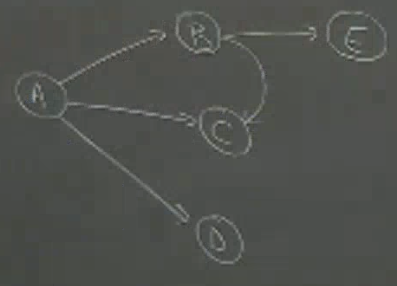
\includegraphics[scale=0.5]{13.png}
\end{center}
A graph have nodes, labels and edges. How to store it? We know to store it as an adjacency list or matrix, typically list for space reasons. An adjacency list is an array of nodes and a list of adjacent nodes for each node. The nodes in the lists are sorted according to some rule. In the example:
\begin{center}
	$\begin{array}{c c l}
	A&\rightarrow&B,C,D\\
	B&\rightarrow&C,E\\
	C&\rightarrow&\\
	D&\rightarrow&\\
	E&\rightarrow&
	\end{array}$
\end{center}
We can't use strings, due to variable length and a lot of pointers. We can assign each node an id, for example $A$ is $1$, $B$ is $2$ and so on based on the order of appearance in the graph. The list will become
\begin{center}
	$\begin{array}{c c c l}
	1&A&\rightarrow&2,3,4\\
	2&B&\rightarrow&3,5\\
	3&C&\rightarrow&\\
	4&D&\rightarrow&\\
	5&E&\rightarrow&
	\end{array}$
\end{center}
Same trick: taking the problem and turning it into the problem of storing sequences of integers, so typically apply Elias-Fano to the adjacency lists. But I could use something more compressed but less powerful, since every time I access the adjacency list I do it from left to right, without the need of NextGeq and other operations. So I could use P for delta or other codes.\\\\
Let's assume we have this tree (with left-right childs that might be null)
\begin{center}
	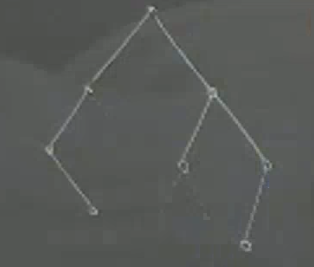
\includegraphics[scale=0.5]{14.png}
\end{center}
With $n=8$ nodes. We could implement it with pointers, every node with a left and right pointer and possibly another pointer for the parent, and with 8 bytes per pointer that's 24 bytes per node just for the structure. We can do better in an elegant and brilliant way, consisting of several steps (\textbf{LOUDS} scheme).\begin{enumerate}
	\item \textbf{Tree completion}: transforming the tree into a full binary tree\begin{center}
		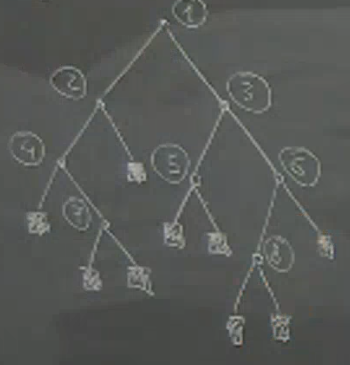
\includegraphics[scale=0.5]{15.png}\\
		The circled numbers are relative to the original tree
	\end{center}
	\item \textbf{Node labeling} for the full binary tree \begin{center}
		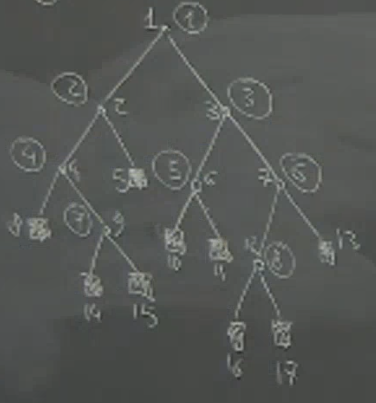
\includegraphics[scale=0.5]{16.png}
	\end{center}
	\item \textbf{Serialization of the node labels} of the full binary tree\\
	$B$ of 17 positions, I scan the tree and every time I find an original node I record 1 and every time I find a dummy node I record 0.
	$$\begin{array}{r c c c c c c c c c c c c c c c c c}
	\text{Positions}&1&2&3&4&5&6&7&8&9&10&11&12&13&14&15&16&17\\
	B = &1&1&1&1&0&1&1&0&1&0&0&1&0&0&0&0&0
	\end{array}$$
	Compress and index $B$ using Rank/Select data structures, using a space of $|B|+o(|B|)$ for Rank$_1$ $+ o(|B|)$ for Select$_1$
\end{enumerate}
$B$ is 17 bits, but where does this number comes from? It's $2n+1$, because we have $n$ ones (original nodes) and $n+1$ dummy nodes. So the space is $2n+1+o(n)$, the lower bound is the \textbf{catalan number}.
\paragraph{Catalan Number} The number of binary trees of $n$ nodes $= 2^{2n}$, then the number of bits surely needed to represent a tree is $\log_2 2^{2n} = 2n$, so you can't do better than $2n$ bits in space. So we are far from the lower bound by $1+o(n)$ bits.\\
$o(n)$ can be interpreted as $o(1)$ bits per node, so I'm far from the lower bound of less than 1 bit per node. This solution is called \textbf{succint}, because it's not compressed but we get the minimum possible plus something that is vanishing.\\\\

Let's see how, in the original tree, \begin{list}{}{}
	\item to take the right child from node $x$
	\item to take the left child from node $x$
	\item to take the parent from node $x$
\end{list}
If we consider $x \rightarrow 2x+1$ it works on the circled nodes to the non-circled nodes (children of $1$ are $2$ and $3$, children of $3$ are $6$ and $7$\ldots). So the right child is $2x + 1$ and the left child is $2x$, both uncircled but I want the circled nodes so from each dummy node I have to find the corresponding original one or a "not existing in the original tree" value. If I take the number 9, for example, I can find it in $B$, which numerations corresponds to the dummy nodes. The corresponding original node is the Rank$_1$, if the value is $1$
$$\begin{array}{r c c c c c c c c c c c c c c c c c}
	\text{Positions}&1&2&3&4&5&6&7&8&9&10&11&12&13&14&15&16&17\\
	B = &1&1&1&1&0&1&1&0&1&0&0&1&0&0&0&0&0\\
	\text{Rank}_1&1&2&3&4& &5&6& & 7 & & & 8\\
	& & & & & & & & &\uparrow
	\end{array}$$
	So I just do Rank$_1(9)$. So the left child is Rank$_1(2x)$ if $B[2x]=1$ and the right child is Rank$_1(2x+1)$ if $B[2x+1]=1$.\\
	The parent comes from inverting the child operations, and it's $\lfloor\frac{\text{Select}_1(x)}{2}\rfloor$. On the uncircled nodes, the parent is the half, but we are reasoning for uncircled values. So first we turn $x$ into an uncircled value, the opposite of before, then we divide by two and find the parent (circled). Of course not in the root, so $x\neq 1$\\
Let's see an algorithm that, given a path $\Pi$ and a tree described by its parameters "\ldots", answers if the requested path exists in the given tree starting from the root or not.
\begin{lstlisting}[style=myPython]
def match(path, ...):
	x = 1
	if (L[1] != path[1]):
		return false
	for i in range(1, len(path)-1):
		l = Rank1(2x)
		r = Rank1(2x+1)
		if (B[2x]=1 and L[l]=path[i+1]):
			x = l
		else if (B[2x+1]=1 and  L[r]=path[i+1]):
			x = r
		else:
			return false
	return true
\end{lstlisting}
With $L$ an array of labels such that the original node with id $i$ has label $L[i]$.
\section{Data Compression}
\paragraph{Families of compressors}\begin{list}{}{}
	\item Statistical Compressors
	\item Lempel-Ziv parsings
	\item Burrows-Wheeler Transform, which we will not see
\end{list}
\subsection{Statistical Compressors}
Most important representatives of statistical compressors, based on frequencies, are Huffman and arithmetic.
\paragraph{Notation}\begin{list}{}{}
	\item $\Sigma$, the alphabet of symbols that we will encode.\\
	Can be binary, formed by bytes, words. What changes is the size and the number of possible values of the symbols: 2 for bits, 256 for bytes, thousands/millions for words. It could be an alphabet of integers, so the size is $\infty$\\
	By changing the alphabet we change how we manage the data. The text \texttt{abaabbaab} can be interpreted with an alphabet of bits, of bytes, of letters, of binomials\ldots in the case of letters we have 5 "a"s and 4 "b"s, but in the case of binomials we have 1 "ab", 2 "aa", 1 "bb" and 1 "b\#". Changing the size of the alphabet can help introducing the "context" around the symbol. With single letters you can permute them in the text and still get the same frequency, but with couple of letters getting the same frequency by randomly shuffling the letters it's harder. The downside is the increasing in size of the alphabet, which we have to take into account when we decompress.\\\\
	In fact, by compressing $T$ we obtain $C(T)$ composed of:
	\begin{list}{}{}
		\item Preamble, which contains infos about $\Sigma$, frequency\ldots\\
		Depends on the family of compressors and also the programmer.
		\item Body, a sequence of bits
	\end{list}
	\item The frequencies can be in a:\begin{list}{}{}
		\item \textbf{Static model}: the frequencies are given, you know the frequencies of each symbol
		\item \textbf{Semi-static} model: the frequencies are computed from the data to compress (like the example before)\\
		You assume that the entire text behaves the same way, but can't take into account variations (for example, first part of the text in english and second part in italian)
		\item \textbf{Dynamic model}: consider a uniform starting model and encode while updating the model
	\end{list}
\end{list}
\paragraph{Huffman algorithm} Greedy but also optimal. It repeats the following step: pick the two lightest symbols (less probability) and merge them in one new symbol whose probability is the sum of the probabilities of the merged symbols.
\subparagraph{Example} $\Sigma=\{a,b,c,d,e,f\}$ with corresponding frequencies of $\{0.05, 0.1, 0.15, 0.3, 0.25, 0.15\}$, so a \textbf{static-model}.\\
So the algorithm starts with $\begin{array}{c c c c c c}
a&b&c&d&e&f\\
0.05&0.1&0.15&0.3&0.25&0.15
\end{array}$ and chooses to merge the two with the lowest probability, $a$ and $b$ obtaining a new symbol with probability $0.15$. Now the choice is between $c,f$ and the new symbol and can pick only two: whatever the choice, the algorithm is optimal, so we can pick the oldest symbols so we merge $c$ and $f$ into a symbol of probability $0.30$. Next choice is the $ab$ symbol and $e$, with a new symbol of $0.4$ probability. Next is $d$ and $cf$, with a probability of $0.6$. We are left with just two symbols, $1.0$ of probability.
\begin{center}
	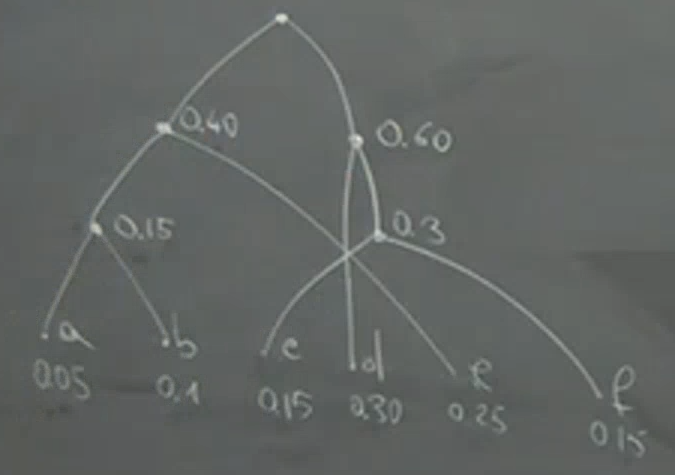
\includegraphics[scale=0.5]{17.png}
\end{center}
The result is a \textbf{binary tree}, which is a way to generate codewords, so codes for symbols. We assign $0$ to the left subtree and $1$ to the right (or viceversa, the order is not important, and can also change the assignment for each subtree). With this we can compute the codewords, from the root to the symbol:
\begin{list}{}{}
	\item \texttt{a} is 000
	\item \texttt{b} is 001
	\item \texttt{c} is 110
	\item \texttt{d} is 10 
	\item \texttt{e} is 01
	\item \texttt{f} is 111
\end{list}
Important things:\begin{list}{}{}
	\item It's a \textbf{prefix-free code}: considering two codewords, no one is a prefix of the other
	\item \textbf{Golden Rule of Data Compression}: the most frequent symbols get the shortest codewords\\
	This because it starts merging from the lightest symbols, which will end up on the bottom of the tree.
\end{list}
To measure the "goodness" of a code we need the \textbf{average codeword length} $L =\sum_\sigma f(\sigma)\cdot l(c_\sigma)$ with $\sigma\in\Sigma$ symbols, $f(\sigma)$ the frequency of the symbol and $l(c)$ the length of its codeword. In our example, $L = 3\cdot0.05 + 3\cdot0.1+3\cdot0.15+2\cdot0.3+2\cdot0.25+3\cdot0.15 = 2.45$ bits.\\\\
Whats the relation between $L$ average codeword length and $h$ height of the tree? $L$ means that on average every symbol will emit $L$ bits. The height of the tree is equale to the codeword length, a $1:1$ relation between length of the codeword and depth of the symbol so that is also called trie of codeword. This means that $L$ can be interpreted, in terms of the height, as the average path length $\equiv$ average depth of the tree.\\\\
For this algorithm, the preable would contain the tree and $\Sigma$. So for the example \texttt{aaabb}, the body would be \texttt{000000000001001}. With \texttt{aaabb} I use 5 bytes, so 40 bits. Now I use 15 bits for the body plus the size of the preamble. So a good comparison is fundamental.
\paragraph{Theorem} Huffman code is optimal among the prefix-free codes for $\Sigma$. In other words $L_H \leq L_C\:\:\forall\:C$ prefix-free code.
\subparagraph{Lemma 1} Let $F$ be the set of binary trees corresponding to optimal prefix-free codes, thus binary trees with minimum average depth. Assuming they have $|\Sigma|$ leafs.\\
$\exists$ tree $\in F\:|$ the minimum weighted leafs are at the largest depth.
\subparagraph{Lemma 2} Considering a tree corresponding to a code $C$, with $x,y$ leafs among the $|\Sigma|$ leafs, and considering its \textbf{reduced tree} $R_C$ with the two leafs $x,y$ merged into a leaf with probability $P(x) + P(y)$ (so that $R_C$ has $|\Sigma|-1$ leafs). We have $L_C  = \sum_{\sigma\neq x,y} l(c_\sigma)\cdot f(\sigma)+l(x)P(x) + l(y)P(y)$ and $L_{R_C}  = \sum_{\sigma\neq x,y} l(c_\sigma)\cdot f(\sigma)+l(\langle x,y\rangle)(P(x)+P(y))$. Given that $l(x) = l(y) = l + 1$ then $l(\langle x,y\rangle) = l$ so that $L_C = L_{R_C} + P(x) + P(y)$
\subparagraph{Proof} The base case in on $|\Sigma| = 2$, obviously optimal. By induction, from $|\Sigma|-1 \rightarrow |\Sigma|$ symbols, assume that Huffman constructs the optimal code for $|\Sigma|-1$ symbols.\\
Let's consider $L_H$, for lemma 2 we have $L_H = L_{R_H} + P(x) + P(y)$, with $x,y$ being the symbols of the smallest frequency merged by Huffman. Let's pick an optimal code, $O$. From lemma 1, there's a tree whose smallest probability leafs are at the deepest level. So in $O$ we know that $x,y$ are at the bottom, and we can apply lemma 2 obtaining $R_O$ with the leafs $x,y$ merged.\\
$H$ and $O$ would have $|\Sigma|$ leafs, and $R_H,R_O$ would have $|\Sigma|-1$ leafs. For inductive hypothesis, we know that Huffman of $|\Sigma|-1$ leafs, so $R_H$, is optimal. So the average depth of $R_H$, which is $L_{R_H}$, is $\leq$ than the average depth of $R_O$. So we have $L_{R_H}\leq L_{R_O}$\\
So we have $L_H = L_{R_H} + P(x) + P(y) \leq L_{R_O} + P(x) + P(y)$ and for lemma 2 we have $= L_O$, concluding that $L_H = L_O$ being that $L_O$ is optimal, proving that Huffman is optimal.
\paragraph{Entropy} The entropy $H = \sum_\sigma P(\sigma)\cdot\log_2\frac{1}{P(\sigma)}$. In Huffman, $L_H = \sum_\sigma P(\sigma)\cdot l(c_\sigma)$.\\
Very similar formulas, differing just by one factor: $\log_2\frac{1}{P(\sigma)}\in R$ and $l(c_\sigma)\in N$, so in general not equal.\\
If the probabilities are diatic, in the form of $2^{-k}$, the two formulas could correspond, but it's not the general case, but surely we have that $$H\leq L_H < H + 1$$ So Huffman loses up to 1 bit per symbol: is this bad or good? This formula is per symbol, let's see it for the entire sequence (multiply by $n$)
$$nH\leq \text{Huffman length} < nH + n$$ So we lose $n$ bits over the overall file. Good or bad depends on $nH$: if very small entropy, so $H$ close to zero meaning the text is highly repetitive, then $+n$ is very large, but if the text is not repetitive, then $n$ is possibly smaller than $nH$ and so it's ok. So the loss depends on the entropy. Arithmetic is able to drop that $+1$.\\
This comes from the \textbf{Shannon bound} ($H\leq L_C$) and it's for all prefix-free code $C$. The property of Huffman is the right part.

\paragraph{Canonical Huffman} We want to create an Huffman code with some properties: more succint in space (not regarding the codewords, which are already optimal, but regarding what we are storing in the preamble) and with an increased speed in the compression.\\
The main idea is to turn the Huffman tree into an unbalanced tree with the deepest codewords in the left part, and the more to the right the less deep it is. A heap-like structure: more to the left, less to the right.
\begin{enumerate}
	\item Build an Huffman tree 
	\item Compute codeword lengths
	\item Compute the number of symbols per level/length (\textbf{num} array)\\
	So for each level, the number of codewords per level
	\item Compute the symbol table (\textbf{symb})\\
	For every level, keep a list of symbols per each level
	\item Computing the new codewords.\\
	It's sufficient to find the first codeword for each level, because all the codewords in that level are increasing\\
	$l =$ max level, the first codeword of level max $fc[l_{max}] = 0$ and $l<l_{max}$ such that $fc([l])=\frac{fc[l+1]+\text{num}[l+1]}{2}$\\
	Mathematically, by summing the first plus the num array element, I'm going to the next available leaf not occupied by any symbol on that level, and dividing by two in binary is just making a shift so we're dropping the leaf and going up one level. So it's the first codeword of the level $+1$ plus the number of leafs divided by two to go to the parent.\\
	With $fc$ and the length which is $l$, we represent the value on $l$ bits and get the codeword.
\end{enumerate}
\subparagraph{An example} For the codeword lengths $\begin{array}{c c}
a & 4\\
b & 4\\
c & 3\\
d & 2\\
e & 2\\
f & 2
\end{array}$ $$\text{num= }\begin{array}{c| c c c c}
\text{pos}&1&2&3&4\\
\hline
\text{val}&0&3&1&2\\
\end{array}\:\:\:\text{symb= }\begin{array}{c| l l l l}
&0&1&2&\ldots\\
\hline
1&\\
2&d,&e,&f\\
3&c\\
4&a,&b
\end{array}$$
$$\begin{array}{r | c c c c}
fc & 1 & 2 & 3 & 4\\
 & \frac{fc[2] + num[2]}{2} = \frac{1 + 3}{2} = 2 & \frac{fc[3] + num[3]}{2} = \frac{1 + 1}{2} = 1 & \frac{fc[4] + num[4]}{2} = \frac{0 + 2}{2} = 1 & 0\\
\text{codeword} & \text{dummy value for the algorithm} & 01 & 001 & 0000
\end{array}$$
The first codeword at the deepest level is $0$, and the levels without codewords are still computed due to the functioning of the algorithm. The values are used as integers, so the $fc[1] = 2$ cannot be represented on $l=1$ bit, but it's not a problem because it's a dummy value and the fact that it's outside the tree is fundamental for the algorithm.
\begin{center}
	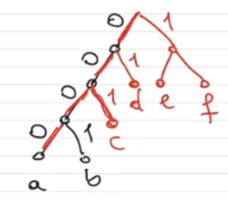
\includegraphics[scale=0.5]{18.png}
\end{center}
So we don't store the tree, we store the first codeword and the number of codewords in each level. To reconstruct the tree, we assign the first symbol to the first codeword and incrementally the rest of the symbols that are left for each codeword on that level, then move up one level to the first codeword of that level and assign the rest of the symbols and so on. So we store $fc$ and $symb$, $num$ is a temporary array just for computing.\\\\
For \textbf{encoding}, given $T=bcf$ we see that $b$ is position/rank 1 of level 4, we take $fc[4] + rank[b] = 0 + 1 = 1$ on $4$ bits so $0001$. Same for $c \Rightarrow fc[3] + rank[c] = 1 + 0 = 1 \Rightarrow 001$\\\\
The space needed is the space for $fc$ plus the space for $symb$ plus the space for the array $symb\rightarrow$ level.\\$fc$ occupies $l_{max}\cdot$ the number of bits to represent the codewords which is at most $l_{max}$, the table $symb$ occupies $|\Sigma|\cdot\log|\Sigma|$ because it is a table of lists containing each symbol that cost $\log|\Sigma|$ to store, the array has to store a level (on $\log_2 l_{max}$ bits) for each symbol, which are $|\Sigma|$, so occupies $|\Sigma|\cdot\log_2 l_{max}$.\\
So the total space is $$l_{max}\cdot l_{max} + |\Sigma|\cdot\log|\Sigma| + |\Sigma|\cdot\log_2 l_{max}$$
The tree has $|\Sigma|$ leafs and $|\Sigma|-1$ internal nodes, so it occupies $2|\Sigma|-1$ pointers, which is a lot more bits.\\\\
For \textbf{decoding}, we can only use $fc$ and $symb$ (the $symb\rightarrow$ level array is not needed for decoding). To decode an array $v$ of $l$ bits, we must check if the node coded by the $l$ bits it's an internal node, so we need to read one more bit and repeat, or if the node is a leaf. We check if the value $v < fc[l]$: if it's less than the first key, it's "on the left" therefore it's an internal node, otherwise it's a leaf therefore we decode it. The dummy node of a level $m$ without leafs it's always greater than any possible value $v$ of the $m$ bits, so we will always "go down". The code:
\begin{lstlisting}[style=myPython]
v = nextBit();
l = 1;
while (v < fc[l]):
	v = 2*v + nextBit();
	l++;
return symb[l][v-fc[l]]
\end{lstlisting}
\subsection{Arithmetic Coding}
\paragraph{Tools for the arithmetic Coding}
$x\in[0,1)$ positional representation for $x$: $.b_1 b_2 \ldots b_k \ldots$ with $b_i$ representing $2^{-i}$, with $b_i\in [0,1]$. These are called \textbf{dyadic fractions}, because are of the form $\frac{v}{2^n}$\\
For example $.101 = \frac{1}{2} + \frac{1}{8} = \frac{5}{8}$\\
To represent, you add zeroes to the binary representation of $v$ until you get $k$ bits: $.0\ldots 0\:bin(v)$ such that the length is $k$ bits. For example, $\frac{5}{16} = \frac{5}{2^4}$ so $5$ in binary over $4$ bits and the dot $\Rightarrow .0101 = \frac{1}{4} + \frac{1}{16} = \frac{4+1}{16} = \frac{5}{16}$\\
We need another tool, which we can use to represent a fraction as a sequence of that type: an algorithm \texttt{converter(x, k)} with $k$ being the precision/accuracy, how many bits we want to use and $x\in[0,1)$. The algorithm works as follows: if $2x < 1$ we output $0$ and repeat on $2x$, else if $2x\geq 1$ we output $1$ and repeat on $2x-1$.\\
An example $x=\frac{1}{3}$\begin{list}{}{}
	\item $2x=\frac{2}{3} < 1 \rightarrow 0$
	\item $2x=\frac{4}{3} > 1 \rightarrow 1$ and $\frac{4}{3} - 1 = \frac{1}{3}$
	\item $2x=\frac{2}{3} \rightarrow 0$
	\item $\rightarrow .\overline{01}$
\end{list}
$x=\frac{5}{8}$\begin{list}{}{}
	\item $2x = \frac{10}{8} > 1 \rightarrow 1$ and $\frac{10}{8} - 1 = \frac{1}{4}$
	\item $2x = \frac{1}{2} < 1 \rightarrow 0$
	\item $2x = \frac{2}{2} = 1 \rightarrow 1$ and $\frac{2}{2} - 1 = 0$
	\item When we have 0 we stay with 0 forever so $\rightarrow .101\overline{0} = .101$
\end{list}
When we stop after $k$ bits we have to compute the error. \textbf{Lemma}: given $x=.b_1b_2\ldots b_d b_{d+1}\ldots$, we compute $\overline{x} = .b_1b_2\ldots b_d0\ldots0$ which is $x$ truncated at the first $d$ digits. So the difference is the value of the bits from $b_{d+1}$ onward, so $$x-\overline{x}=\sum_{i=1}^\infty b_{d+i}\cdot 2^{-(d+i)} = 2^{-d}\cdot\sum_{i=1}^\infty b_{d+i}\cdot 2^{-i}\leq 2^{-d}\cdot\sum_{i=1}^\infty 1\cdot 2^{-i} = 2^{-d}$$
Because the worst case is when every $b_i$ with $i\geq d+1$ is $1$ and $t\sum_{n=1}^\infty \frac{1}{2^n} = 1$. This means that \texttt{converter(x, k)} makes an error of at most $2^{-k}$
\paragraph{Arithmetic coding} Let's assume we have an alphabet of 3 symbols with $P(a) = \frac{1}{2}, P(b) = P(c) = \frac{1}{4}$. We assume to map the symbols in the $[0,1)$ interval alphabetically and according to the probability. So $f_a = 0, f_b = \frac{1}{2}, f_c = \frac{3}{4}$ are the cumulative frequencies of the previous symbols. $a$ is the first so $0$, $b$ is preceeded by $a$ so is $P(a)$, $c$ so is $P(a)+P(b)$. We do some trivial (for computers) calculation on the interval, depending on the text.\\
Let's assume $T = abca$\begin{list}{}{}
	\item The size at the beginning is the size of the whole interval $[0,1)$, so $s_0 = 1$
	\item The first symbol is $a$, we go in its interval which is $[0,\frac{1}{2})$ and the size of the new interval is $s_1 = s_0\cdot P(a) = \frac{1}{2}$. This new interval must be partitioned according to the probabilities, so the first partition is of size $P(a)=\frac{1}{2}$ of the current interval so it's $\frac{1}{4}=s_1\cdot P(a)$, the second and third are of size $P(b)=P(c)=\frac{1}{4}$ so they are $\frac{1}{8} = s_1\cdot P(b) = s_1\cdot P(c)$\\
	The first value, the border between the first two partitions, is $0$ (the beginning of the new interval) $+$ the size of the first partition $\frac{1}{4} = \frac{1}{4}$, the second border value is $0+\frac{1}{4}$ for the first partition $+\frac{1}{8}$ for the second $=\frac{3}{8}$, then the last border is the last value which is $\frac{1}{2}$\\
	Programmatically, the interval starts at $0+f_a\cdot s_1 = 0$. The second partition starts at $0+f_b\cdot s_1 = 0+\frac{1}{2}\cdot\frac{1}{2} = \frac{1}{4}$ and so on. So the starting position of a letter is the current size times the cumulative frequency of that letter.
	\item The second symbol is a $b$, so we zoom in it's interval inside $s_1$, which goes from $[\frac{1}{4},\frac{3}{8})$ of size $s_2 = s_1\cdot P(b) = \frac{1}{2}\cdot\frac{1}{4} = \frac{1}{8}$ and we partition in three parts again like before. The first partition is again for $a$ and starts at $\frac{1}{4}$, the beginning of the interval. The second partition, of $b$, starts at $\frac{1}{4}+f_b\cdot s_2 = \frac{1}{4}+\frac{1}{2}\cdot\frac{1}{8} = \frac{5}{16}$ and the third starts at $\frac{1}{4} + f_c\cdot s_2 = \frac{11}{32}$
\end{list}
So the arithmetic coding keeps the two integers describing the interval $[l_n, l_n+s_n)$: the left and the right endpoints of the interval. We start with $l_0 = 0, s_0 = 1$, and in every step $s_{n+1} = s_n\cdot P(T[n+1])$ and $l_{n+1} = l_n + f_{T[n+1]} \cdot s_n$, with $T[n+1]$ being the character in position $n+1$ which we are encoding.
\paragraph{What Arithmetic Coding Sends on the Network} Let's start with an example: $T=abac\longrightarrow$ will output $\left[\frac{19}{64},\frac{5}{16}\right)$. With a semi-static model, where we count occurrences, $f(a)=\frac{2}{4} = \frac{1}{2}$, $f(b)=f(c)=\frac{1}{4}$. Arithmetic coding sends the number in the middle of the interval, so in this case the size of the interval is $s=\frac{1}{64}$, the left extreme is $l=\frac{19}{64}$ therefore the picked number is $= l + \frac{s}{2} = \frac{19}{64}+\frac{1}{128} = \frac{39}{128}$. To represent this number we can do the classical representation of $\frac{v}{2^k}$ which is $bin(v)$ over $k$ bits, but we could do with less bits. So we represent a truncation of the number but guaranteeing that the truncation is larger than $l$.\\
Remember we send the number and the length of $T$, because the number could correspond to an infinite number of texts.
\subparagraph{Theorem} We truncate to $d=\lceil\log_2\frac{2}{s}\rceil$ bits. The truncated number converter($l+\frac{s}{2},d$)$\in[l,l+s)$.\\
Remember that, according to a lemma, the number of information lost due to truncation at $d$ bits is $2^{-d}$.
$$2^{-d} = 2^{-\lceil\log_2\frac{2}{s}\rceil} = \frac{1}{2^{\lceil\log_2\frac{2}{s}\rceil}}\leq \frac{1}{2^{\log_2\frac{2}{s}}} = \frac{1}{\frac{2}{s}} = \frac{s}{2}$$
So this is a safe truncation, the number is still $\geq l$.\\\\
In the example $d = \lceil \log_2 \frac{2}{s}\rceil = \lceil\log_2\frac{2}{\frac{1}{64}}\rceil = \lceil\log_2 128\rceil = 7$ bits, so we do converter($\frac{39}{128},7$) $= 0100111$ which is just $39$ over $7$ bits but it's a particular case, $39$ can be represented over $7$ bits without truncation.
\paragraph{How good is the arithmetic compressor?} For Huffman, we had $H\leq L_{Huff} < H+1$ bits, giving Huffman compression $< nH+n$ with $n=|T|$, because Huffman can only use an integer number of bits per codeword while the entropy $H$ uses real numbers.\\
Arithmetic compression $< nH + 2$, with a theoretical constant $2$ in the case of infinite arithmetic precision. In reality, it's something like $< nH + c\cdot n$ with $c\simeq\frac{1}{100}$.
\subparagraph{Theorem} $d< nH + 2$
$$d = \lceil\log_2\frac{2}{s}\rceil = \lceil 1-\log_2 s\rceil < 2 - \log_2 s = 2-\log_2\prod_{i=1}^{|T|}p(T[i]) = 2 - \sum_{i=1}^{|T|} \log_2 p(T[i]) =$$
In the previous example of $T = abac$ this would be $=2- [\log_2 p(a)+\log_2 p(b)+\log_2 p(a) + \log_2 p(c)] = 2 - [2\cdot\log_2 p(a) + 1\cdot\log_2 p(b) + 1\cdot \log_2 p(c)$ so the number of occurrences times the probability
$$ = 2 - \sum_\sigma \text{occ}(\sigma)\cdot\log_2 p(\sigma) = 2 - n\cdot\sum_\sigma \frac{\text{occ}(\sigma)}{n}\cdot\log_2 p(\sigma) = $$
For sufficiently large texts, the number of occurrences occ($\sigma$) over $n$ converges to the frequency of $\sigma$ $f(\sigma)$, and in the semi-static model $p(\sigma)$ is $f(\sigma)$ 
$$2 - n\sum_\sigma p(\sigma)\cdot\log_2 p(\sigma) = 2 + n\sum_\sigma p(\sigma)\log_2\frac{1}{p(\sigma)}$$ and $H = \sum_\sigma p(\sigma)\log_2\frac{1}{p(\sigma)}$.\\\\
Recently, ANS (Asymmetric Numeral Systems) was proposed as a variation of the Arithmetic Encoding we've seen and it's actually better than this bound.\\\\
So in every case you have to look at the entropy: if it's very small, so the source is highly compressible, then the $nH$ part is close to $0$ and additive part $+n$ or $+c\cdot n$ makes the difference. When the entropy is very large then $nH$ dominate and we can use Huffman.
\paragraph{Decoding} Whenever we decompress, we have the preamble and the body of the compressed file. The preamble of the arithmetic encoders usually consists of the probabilities of the symbols and the length of the text.\\
For example $P(a) =\frac{1}{2}, P(b)=P(c)=\frac{1}{4}$ and the text length $= 2$ with the body being $(111)_2$. The first thing to do is to transform the body into a real number (keeping the fraction, because then it's easier to do the calculations by hand): $(111)_2 = .111 = \frac{1}{2} + \frac{1}{4} + \frac{1}{8} = \frac{7}{8}$.\\
Now we start from $[0,1)$ and partition according to the probabilities: from $0$ to $\frac{1}{2}$ is $a$, from $\frac{1}{2}$ to $\frac{1}{2}+\frac{1}{4}=\frac{3}{4}$ is $b$ and from $\frac{3}{4}$ to $\frac{3}{4} +\frac{1}{4} = 1$ is $c$. With $\frac{7}{8}$ we go in the $c$ partition (zoom into $[\frac{3}{4},1]$) and partition. Now the size is $s_1 = \frac{1}{4}$ so $a$ goes from the beginning $\frac{3}{4}$ to $\frac{3}{4} + s_1\cdot P(a) = \frac{3}{4} + \frac{1}{4}\cdot\frac{1}{2} = \frac{7}{8}$, same reasoning for $b$ which goes from $\frac{7}{8}$ to $\frac{15}{16}$.\\
Every interval is closed below and open up, so $\frac{7}{8}$ belongs to the interval $b$. We stop because we found text len $=2$ symbols, and return $T=cb$.
\subsection{Lempel-Ziv Family}
\paragraph{LZ Compressors}
\begin{enumerate}
	\item Parsing, transform the text into a sequence of triples.
	\item Encoding
\end{enumerate}
\paragraph{Parsing} $T=aacaacab|caaaaaaac$, where we've compressed up until the line and need to compress the next part. So the first part is the \textbf{dictionary}, all the substrings that starts in the first part are the dictionary. It parses the next part and finds the longest substring that starts in the first part:
\begin{list}{}{}
	\item $c$ is in the first part
	\item $ca$ too
	\item $caa$ too
	\item $caaa$ doesn't
\end{list}
So it takes $caa$ plus one character: $caaa$ is called a \textbf{phrase}, it's represented as a copy of the corresponding substring in the dictionary, and is represented with $\langle d,l,$ char$\rangle$ corresponding to the distance of the copy (in this case, from $caa$, so $d=6$), the length ($caa$ has $l=3$) and the next character ($a$). We then move the bar after the $a$ and repeat for $T=aacaacabcaaa|aaaac$.\\
Now the important part is that the copy start before: in this case, we have 4 $a$s, copied beginning from just the last $a$ before the bar: we copy $T=aacaacabcaaa|\underline{aaaa}c$ from $T=aacaacabcaa\underline{a|aaa}ac$ and it's not important that overlaps, becoming $\langle 1,4,c\rangle$\\\\
What happens at the beginning? We start from $T=|aacaacabcaaaaaaac$, encode $\langle 0,0, a\rangle$ and the bar goes after the last character encoded so $T=a|acaacabcaaaaaaac$. We emit $\langle 1,1,c\rangle$ and $T=aac|aacabcaaaaaaac$, then $\langle 3, 4, a\rangle$ giving $T=aacaaca|bcaaaaaaac$ and so on.
\paragraph{Encoding} The crucial part is how to encode the numbers and the characters, we cannot represent them in full because we can end up with a larger space complexity than the original data.\\
For example, we could define three "texts": \begin{list}{}{}
	\item text of distances $T_{dist} = 01361$
	\item text of lengths $T_{len} = 01434$
	\item text of characters $T_{char} = acaac$
\end{list}
and we could encode these three texts in any way we want as seen before.
\paragraph{Window to copy} Whenever we look for a substring in the dictionary to copy, we cannot look arbitrarily back: typically the compressors have a window of words of length $w$ and we consider only copies that starts at most $w$ character before so $d\leq w$. In \texttt{gzip} we have options \texttt{-1},\ldots,\texttt{-9} which specifies the windows from 100 Kb to 900 Kb. The larger the windows the more you compress, so less phrases and \textbf{faster in decompression} because every phrase tells you to go back and copy, it's a random jump, so with less random jumps the caching is more effective. But with larger windows we have \textbf{slower compression}.\\\\
The approach discussed is called \textbf{LZ 77}.
\paragraph{How to find the copies} There are several algorithms in literature, let's see the one used by \texttt{gzip} due to it being interesting from a programming point of view. Let's say we are in the situation $T = \:\:\:\:\:\:\:\:\:\:|caaa\ldots$: a brute-force way would be to take $c$ and search for it going back and find it, then take $ca$ and go back and search and find it so on until we don't find the occurrence of the substring. This is really slow, we need something faster: filtering. We want to find the candidate positions and then check them. So I want some tool that tells me the (hopefully few) interesting positions to check. This filter can be built with an hashtable over triples of characters. Let's see an example with $w=7$: $T = acaacab|caaa\ldots$ from position $2,3,4,5,\ldots$. For every previous position, it keeps a key in the hashtable of three characters:\begin{list}{}{}
	\item $\langle bca,8\rangle$
	\item $\langle abc,7\rangle$
	\item $\langle cab,6\rangle$
	\item $\langle aca,5\rangle$
	\item $\langle aac,4\rangle$
	\item $\langle caa,3\rangle$
	\item $\langle aca,2\rangle$
\end{list}
So we can already see that two $aca$s will collide in the same slot, and we have to keep both satellite informations $5$ and $2$. \texttt{gzip} finds copies only if they are longer or equal than three characters: it's useless to substitute one or two characters with a triple.\\
So it takes the next three characters $caa$ and look for in the hashtable: it can find a collision, for example $\langle caa,3\rangle$, $\langle aac, 4\rangle$ and $\langle cab,6\rangle$ can collide, these are the candidate positions so it compares over them.\\
After encoding the triple, we shift the window so the table is cut: each triple points to the next one so we can start from the head and simply cancel triples. We of course also add the new triples.
\paragraph{LZSS} Doesn't use triples but pairs by making the following observation: either we copy, because $d>0$ or we don't copy and meet one single character. So whenever $d=0$ only the character is significant, and whenever we copy the character is useless. So LZSS considers just $\langle d,l\rangle$ (no extra characters) or $\langle 0,$ char$\rangle$.\\So for example $T=aacaacabcaaaaaaac$ we emit $\langle 0,a\rangle$ and $T=a|acaacabcaaaaaaac$, we can only copy $a$ so we output $\langle 1,1\rangle$ and $T=aa|caacabcaaaaaaac$, then $\langle 0,c\rangle$ and $T=aac|aacabcaaaaaaac$, then we can copy $aaca$ starting from the beginning ($3$ characters before) and copying 4 characters, so we output $\langle 3,4\rangle$ and $T=aacaaca|bcaaaaaaac$.\\
The decoder expects pairs, reads the first number and if it's zero then knows that the next element is a character, otherwise knows that the next one is a number.
\paragraph{LZ78} Different dictionary, this time is explicit. $T=aabaacabcabcb$, we have and output and a explicitly constructed dictionary that starts with $\epsilon$, the empty string.

\begin{multicols}{2}
\begin{list}{}{\textbf{Output}}
	\item $T=aabaacabcabcb$
	\item Since we don't find anything in the dictionary, which at this time is just the node $0$ corresponding to $\epsilon$, we emit $\langle 0, a\rangle$ and since we are processing one character we append it to the dictionary.
\end{list}
\columnbreak
\begin{center}
	\begin{tikzpicture}[node distance={15mm}, main/.style = {draw, circle}] 
	\node[main] (1) {0};
	\node[main] [below left of=1] (2) {1};
	\draw[->] (1) -- (2) node [pos=0.5, right] {$a$};
\end{tikzpicture}
\end{center}
\end{multicols}
\begin{multicols}{2}
\begin{list}{}{}
	\item $T=a|abaacabcabcb$
	\item We start from the root, match $a$ and can't find $b$ so we stop after $b$, emit $\langle 1,b\rangle$ and add $b$ to the trie.
\end{list}
\columnbreak
\begin{center}
	\begin{tikzpicture}[node distance={15mm}, main/.style = {draw, circle}] 
	\node[main] (1) {0};
	\node[main] [below left of=1] (2) {1};
	\draw[->] (1) -- (2) node [pos=0.5, right] {$a$};
	\node[main] [below left of=2] (3) {2};
	\draw[->] (2) -- (3) node [pos=0.5, right] {$b$};
\end{tikzpicture}
\end{center}
\end{multicols}
\begin{multicols}{2}
\begin{list}{}{}
	\item $T=aab|aacabcabcb$
	\item We have $aa$, find just one $a$ so we encode $\langle 1,a\rangle$ and add the second $a$ to the first $a$ subtree.
\end{list}
\columnbreak
\begin{center}
	\begin{tikzpicture}[node distance={15mm}, main/.style = {draw, circle}] 
	\node[main] (1) {0};
	\node[main] [below left of=1] (2) {1};
	\draw[->] (1) -- (2) node [pos=0.5, right] {$a$};
	\node[main] [below left of=2] (3) {2};
	\draw[->] (2) -- (3) node [pos=0.5, right] {$b$};
	\node[main] [below right of=2] (4) {3};
	\draw[->] (2) -- (4) node [pos=0.5, right] {$a$};
\end{tikzpicture}
\end{center}
\end{multicols}
\begin{multicols}{2}
\begin{list}{}{}
	\item $T=aabaa|cabcabcb$
	\item We have no $c$ from the root, encode $\langle 0,c\rangle$ and add it to the root.
\end{list}
\columnbreak
\begin{center}
	\begin{tikzpicture}[node distance={15mm}, main/.style = {draw, circle}] 
	\node[main] (1) {0};
	\node[main] [below left of=1] (2) {1};
	\draw[->] (1) -- (2) node [pos=0.5, right] {$a$};
	\node[main] [below left of=2] (3) {2};
	\draw[->] (2) -- (3) node [pos=0.5, right] {$b$};
	\node[main] [below right of=2] (4) {3};
	\draw[->] (2) -- (4) node [pos=0.5, right] {$a$};
	\node[main] [below right of=1] (5) {4};
	\draw[->] (1) -- (5) node [pos=0.5, right] {$c$};
\end{tikzpicture}
\end{center}
\end{multicols}
\begin{multicols}{2}
\begin{list}{}{}
	\item $T=aabaac|abcabcb$
	\item We find $ab$ in the trie, so we emit $\langle 2,c\rangle$ and add $c$ to the $b$ subtree
\end{list}
\columnbreak
\begin{center}
	\begin{tikzpicture}[node distance={15mm}, main/.style = {draw, circle}] 
	\node[main] (1) {0};
	\node[main] [below left of=1] (2) {1};
	\draw[->] (1) -- (2) node [pos=0.5, right] {$a$};
	\node[main] [below left of=2] (3) {2};
	\draw[->] (2) -- (3) node [pos=0.5, right] {$b$};
	\node[main] [below right of=2] (4) {3};
	\draw[->] (2) -- (4) node [pos=0.5, right] {$a$};
	\node[main] [below right of=1] (5) {4};
	\draw[->] (1) -- (5) node [pos=0.5, right] {$c$};
	\node[main] [below left of=3] (6) {5};
	\draw[->] (3) -- (6) node [pos=0.5, right] {$c$};
\end{tikzpicture}
\end{center}
\end{multicols}
\begin{multicols}{2}
\begin{list}{}{}
	\item $T=aabaacabc|abcb$
	\item We emit $\langle 5,d\rangle$ and add $d$ trie (although it's useless since we've finished)
\end{list}
\columnbreak
\begin{center}
	\begin{tikzpicture}[node distance={15mm}, main/.style = {draw, circle}] 
	\node[main] (1) {0};
	\node[main] [below left of=1] (2) {1};
	\draw[->] (1) -- (2) node [pos=0.5, right] {$a$};
	\node[main] [below left of=2] (3) {2};
	\draw[->] (2) -- (3) node [pos=0.5, right] {$b$};
	\node[main] [below right of=2] (4) {3};
	\draw[->] (2) -- (4) node [pos=0.5, right] {$a$};
	\node[main] [below right of=1] (5) {4};
	\draw[->] (1) -- (5) node [pos=0.5, right] {$c$};
	\node[main] [below left of=3] (6) {5};
	\draw[->] (3) -- (6) node [pos=0.5, right] {$c$};
	\node[main] [below left of=6] (7) {6};
	\draw[->] (6) -- (7) node [pos=0.5, right] {$b$};
\end{tikzpicture}
\end{center}
\end{multicols}
The tries of course is then dropped and we just encode the sequence of pairs: we have two texts (node numbers and characters) that can be encoded as we like.
\paragraph{ZLIB} Implementation of LZ77 which requires the array to compress $A$, its length $n$, and an array of output Out of length $m$ passed as a pointer (so \&$m$) initialized as $m=1.2\cdot n$ so a 20\% increase in size of $A$. This because the system can't know if $A$ is compressible or not, so the extra size is to account for the uncompressible cases (more because we use pairs or triples). When the procedure returns, $m$ has been updated with the occupied size which, possibly, is much smaller than $1.2\cdot n$
\subsection{The Suffix Array}
\paragraph{Notations} Pattern $P$ occurs at position $i$ of $T\Leftrightarrow P$ is a prefix of the $i$-the suffix of $T$ (i.e. $T[i,N]$)\begin{center}
	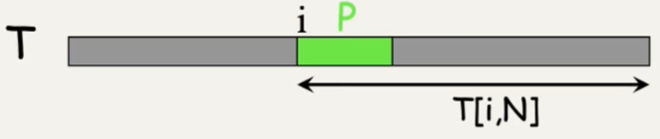
\includegraphics[scale=0.75]{19.png}
\end{center}
So we can transform the problem of searching for occurrences into a problem of searching for prefixes. Occurrences of $P$ in $T$ are all the suffixes of $T$ having $P$ as a prefix.\\
SUF$(T)$ = sorted set of all suffixes of $T$. Algorithmic reduction from substring search to prefix search: for example, using the trie data structure. We have a problem in space, because the total length of the suffixes is $n^2$.\\
We consider an ending character, which sometimes is noted as $\#$ and sometimes as $\$$. So for example $T =$ mississipi$\# \Rightarrow$ SUF$(T)$:
\begin{multicols}{2}
\begin{list}{}{}
	\item \texttt{\#}
	\item \texttt{i\#}
	\item \texttt{ippi\#}
	\item \texttt{issippi\#}
	\item \texttt{ississippi\#}
	\item \texttt{mississippi\#}
	\item \texttt{pi\#}
	\item \texttt{ppi\#}
	\item \texttt{sippi\#}
	\item \texttt{sissippi\#}
	\item \texttt{ssippi\#}
	\item \texttt{ssissippi\#}
\end{list}
\end{multicols}
So all suffixes in SUF$(T)$ having prefix $P$ are in a contiguous portion of the sorted set. Also the starting position of the contiguous portion is the lexicographic one of $P$, meaning that if I can find the position of my prefix in SUF$(P)$ I can simply scan ahead to find all the suffixes with $P$ prefix. So we can consider the suffix array, where every element is a pointer to the position in $T$:
\begin{list}{}{}
	\item 12, 11, 8, 5, 2, 1, 10, 9, 7, 4, 6, 3
\end{list}
The suffix array $SA$ occupies a lot less space than the $n^2$ of SUF$(T)$, it's $O(n)$ in $n = |T|$ and every element is a number of at most $\log_2 n$ bits, so is $\Theta(n\log_2 n)$ bits. In practice, is $5n$ bytes.\\\\
To look for a pattern, indirected binary search on SA: $O(p) = O(|P|)$ time per suffix comparison. So go in the middle element, compare $P$ to the substring pointed by the element and so on, binary search. The total search cost is $O(p\log_2 n)$ time.\\
Listing the occurrences is easy: take the element, access the position and compare, and go to the next element if the comparison is successful. This costs the number of occurrences times $p$, which can be costly with many occurrences. We can speed this up by finding the entire block: we look for $P\#$ with $\#<\sigma\:\:\forall\:\sigma\in\Sigma$ and for $P\$$ for $\sigma < \$\:\:\forall\sigma\in\Sigma$. Therefore, the block of occurrences of $P$ is delimited by those two elements.
\begin{center}
	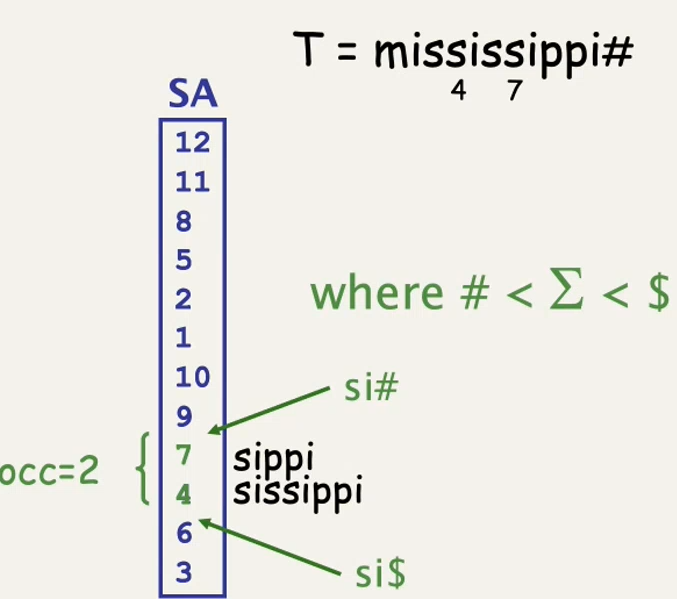
\includegraphics[scale=0.5]{20.png}
\end{center}
With a total time of $O(p\log_2 n +$ occ$)$.
\paragraph{Longest Common Prefix Array} The LCP array has elements that indicates the length of the longest prefix shared by adjacent suffixes. For example, the first and second suffixes in SA share no prefix (the first is "\#" and the second is "i\#"), so the first element of LCP is 0. LCP:
\begin{list}{}{}
	\item 0, 0, 1, 4, 0, 0, 1, 0, 2, 1, 3
\end{list}
How long is the common prefix between $T[i,\ldots]$ and $T[j,\ldots]$? The minimum element between them in LCP, so for example between $5$ and $10$ the common prefix is long $0$ characters. So the min of the subarray LCP[$h,k$] such that SA$[h]=i$ and SA$[k]=j$.
\subsection{Burrows-Wheeler Transform}
\paragraph{Two very simple compressors}
\begin{list}{}{}
	\item \textbf{MTF} Move-To-Front\\
	Start with a list of symbols, a text $L=[a,b,c,d,\ldots]$ and for each input symbol $s$:
	\begin{enumerate}
		\item Output the position of $s$ in $L$
		\item Move $s$ to the front of $L$
	\end{enumerate}
	For example, $L=[a,b,c,l], S =$ cabala $\Rightarrow$ MTF($S$) = 3 2 3 2 4 2.\\
	It's a \textbf{dynamic code} (the same letter can be encoded with different values) and has memory (if the symbol has been read recently, its number will be small).
	\item \textbf{RLE} Run-Length-Encoding\\
	Specifically designed for spacial locality.\\
	Example: $abbbaacccca \Rightarrow (a,1),(b,3),(a,2),(c,4),(a,1)$\\
	In binary string just numbers and the first bit is sufficient.\\
	\textbf{RLE0} is the following pipeline: add $1$ to non-zero elements and encode 0-runs with Wheeler's code.
\end{list}
\paragraph{Wheeler's Code} To encode the sequence of zeroes we do the following: we take the length of the sequence, $n$, and compute Bin$(n+1)$. We use the returned sequence without the first $1$.\\
For example, RLE0(221200) = 33231 because 00 has length $n=2$ and Bin(3) = 11.
\paragraph{Burrows-Wheeler Transform} Let's take a given text $T=$ mississippi\# and we start by rotating $T$:
\begin{list}{}{}
	\item \texttt{mississippi\#}
	\item \texttt{ississippi\#m}
	\item \texttt{ssissippi\#mi}
	\item \texttt{sissippi\#mis}
	\item \texttt{issippi\#miss}
	\item \texttt{ssippi\#missi}
	\item \texttt{sippi\#missis}
	\item \texttt{ippi\#mississ}
	\item \texttt{ppi\#mississi}
	\item \texttt{pi\#mississip}
	\item \texttt{i\#mississipp}
	\item \texttt{\#mississippi}
\end{list}
This produces $|T|$ rows, giving a square matrix (\textbf{BWT matrix}). The we sort the rows (\# is the smallest character):
\begin{list}{}{}
	\item \texttt{\# mississipp i}
	\item \texttt{i \#mississip p}
	\item \texttt{i ppi\#missis s}
	\item \texttt{i ssippi\#mis s}
	\item \texttt{i ssissippi\# m}
	\item \texttt{m ississippi \#}
	\item \texttt{p i\#mississi p}
	\item \texttt{p pi\#mississ i}
	\item \texttt{s ippi\#missi s}
	\item \texttt{s issippi\#mi s}
	\item \texttt{s sippi\#miss i}
	\item \texttt{s sissippi\#m i}
\end{list}
Again a square matrix. We notice that the first column, $F$, is ordered and contains all the characters of $T$: this because we are considering circling rotations and fixing a column every character will pass by that column. We cannot compress just $F$ because every text comprised of those characters (in the example, 4 "i"s, 1 "m", 2 "p"s and 4 "s"s) would give the same $F$. The trick is done with $L$, the column of the last characters: the transformation is invertible if we consider the sequence of characters in the last column.\\
So given a string $T$, we return $L$, which in this case $L=$ ipssm\#pissii.\\\\
Note that the character in $L$ is the one that precedes the character in $F$. With "mississippi" this transformation can't show its true power. With natural language texts, there are a certain number of characters that precedes other characters: for example, in english the letter "n" succeeded by a space can be preceded by an "a", an "o" and other few vowels ("an", "on", "in"\ldots), so in these portions of texts the array $L$ will contain just few repeated characters. This means that \textbf{$L$ is locally homogeneous}, so is \textbf{highly compressible}.
\paragraph{Bzip Algorithm}
\begin{enumerate}
	\item Move-to-Front of $L$
	\item Run-Length coding
	\item Statistical coder
\end{enumerate}
\paragraph{Computing the BWT matrix} If we look at the matrix and notice the position of \#, we notice that we need to sort just the suffixes of $T$: \begin{list}{}{}
	\item \textbf{\#}mississipp i
	\item \textbf{i\#}mississip p
	\item \textbf{ippi\#}missis s
	\item \textbf{issippi\#}mis s
	\item \textbf{ississippi\#} m
	\item \textbf{mississippi} \#
	\item \textbf{pi\#}mississi p
	\item \textbf{ppi\#}mississ i
	\item \textbf{sippi\#}missi s
	\item \textbf{sissippi\#}mi s
	\item \textbf{ssippi\#}miss i
	\item \textbf{ssissippi\#}m i
\end{list}
So \# is a dividing character. So these are the sorted suffixes of $T$, and we can compute it with a suffix array ($SA$) construction algorithm, with a linear space instead of quadratic. Given the items of the $SA$, the corresponding item of $L$ is $L[i] = T[SA[i]-1]$. This requires many jumps in memory, so it's the main reason why bzip is significantly slower than gzip. So this spurred a number of publications in '94-'10 on SA construction.\\
$BW(S) = \langle L$ without $\#$, position of $\#$ in $L\rangle$ with $L$ being the last column. In the example, $BW(S) = \langle$ipssmpissii, 5$\rangle$
\subparagraph{SA with qsort} Initialize the array with the text $T$ and then just sort with qsort. The difference is that every position is treated as a suffix, not as a character. So with qsort we will sort every suffix (from position $i$ of the original $T$ up to the \#), giving $SA$ at the end of the procedure.\\
The procedure is inefficient: $\Theta(n^2\log n)$ in the worst case with $\Theta(n\log n)$ cache misses.
\paragraph{L$\rightarrow$F Mapping} Can we map $L$'s characters onto $F$'s characters? Need to distinguish between equal characters. Every column $i$ is a permutation of the original $T$ given by the first $i-1$ characters. Given a character on $L$, I have to find the equal character on $F$, so I will know the previous character. Iterating this procedure gives the original $T$ from right to left.\\
Taken two characters in $L$, e.g. two "i"s, the first to appear in $L$ is alphabetically smaller than the second. I bring each character to the front of its corresponding rectangle: the alphabetical order doesn't change.
\begin{center}
	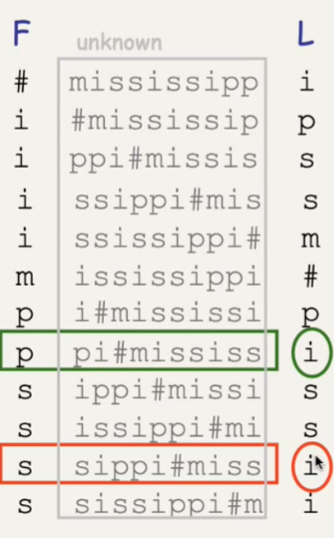
\includegraphics[scale=0.5]{21.png}
\end{center}
Each row will correspond to another row with the rotated character in $F$ and another character in $L$ which is the previous character. Notice that the rows may come closer, but the green will always come before the red.
\begin{center}
	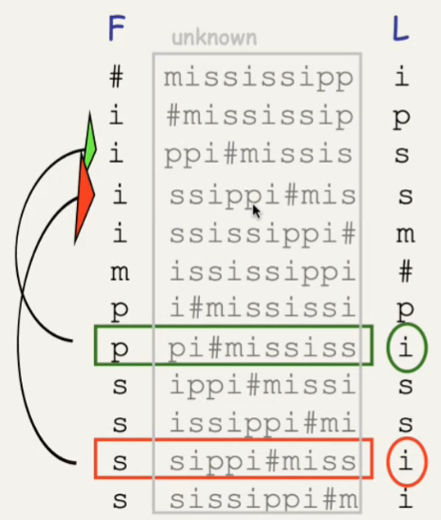
\includegraphics[scale=0.5]{22.png}
\end{center}
These stability in the ordering guarantees that the mapping is trivial.
\begin{center}
	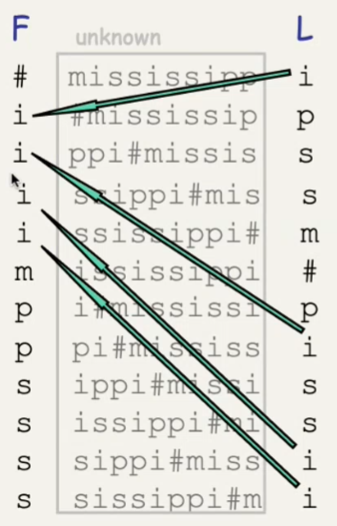
\includegraphics[scale=0.5]{23.png}
\end{center}
These operations are just Rank$_{char}$(pos) and Select$_{char}$(pos) and the reason why these operations are so popular nowadays. Rank$_i$(pos) tells how many "i"s are above pos.
\paragraph{Decompression} After decompressing in the inverse order of the compression, we end up with $L$.\\
First thing to do is to find $F$: sort $L$ and find $F$. We now need to construct the string, and the first character from which we start, constructing from right to left, is \# which is the first character of $F$. So the last character of $T$ is the corresponding character in $L$, which in the example is an "i". Whenever I have an item in $L$, I compute the corresponding character in $F$ and iterate. The corresponding "i" in $F$ of the first "i" in $L$ is the first $i$ we find in $F$, in the second row. And so on.\\
Several issues regarding efficiency in time and space.
\section{Hashing and Dictionary Problem} 
\paragraph{Hashing} Typically related to the \textbf{Dictionary problem}: we have a set of objects $D=\{o_1,\ldots,o_n\}$ with every $o_i$ associated to $\langle$key, satellite information$\rangle$. We want to solve queries like:
\begin{list}{}{}
	\item Membership$(k)$: is $k\in D$?
	\item Insertion$(k)$: $D = D \cup \{k\}$
	\item Deletion$(k)$: $D = D \setminus \{k\}$
\end{list}
The hashing function $h : U\rightarrow [0, m-1]$ from the universe $U$, with a table $T[0,m]$. The hash function is applied to the key which gives a position inside the table. Two objects can collide in the same position, and stay "outside" the table in a overflow list. This is called \textbf{hashing with chaining}. If $U$ is small, then a direct table is better.\\
This approach has a space complexity of the size of the table ($m$) plus the number of objects outside the table ($n$), so $O(m+n)$. Note that $m$ are pointers, the cells of the table, while $n$ are pointers and keys: if the key is an integer then is 4-8 bytes like the pointers, but if it's a string then it's another pointer.\\
\textbf{Loading factor} $\alpha = \frac{n}{m}$, ratio between the number of keys and the size of the table.
\paragraph{Analysis} Up until now in our studies we've seen $h$ that were \textbf{simple uniform hashing}, meaning that\\$\forall\:k\:\:\:P(h(k) = i)=\frac{1}{m}$. This is means that every key is independent and is \textbf{computationally unfeasible}, although possible it takes too much space and time. Let's consider this kind of function.\\\\
The insertion is $O(1)$ because we simply append in $T$.\\
The Membership and Deletion both require a search, and the search costs the average overflow list length: a constant time to access the position required and a scan of the list in that position to search for the key.\\
The average list length is $$E[\text{length of a list}]=\sum_{k'\in D\:k'\neq k} P(h(k')=h(k)) = \sum_{k'\in D\:k'\neq k} P(h(k')=i) = \sum_{k'\in D\:k'\neq k} \frac{1}{m} = \frac{n}{m} = \alpha$$
So the average time for a search is the loading factor $\alpha$. Typically we assume that the computation of $h(k)$ is $O(1)$ so the cost of both Membership and Deletion is $O(1+\alpha)$ to account for the computation.\\\\
If the size of the table is chosen proportional to $n$ then $\alpha$ is constant. We have a problem: how much is $n$? It's certainly dynamic.
\paragraph{Constant Time in Dynamic Context} Let's consider the evolution over time. At the beginning, $t=0$ we have $n_0$ keys and a table of size $m_0 = 2n_0$ so we allocate a table of twice the size, meaning $\alpha_0 = \frac{1}{2}$. Then we add and delete keys.\\
Let's consider a time $t=1$ where either \# keys $\geq 2n_0$ or \# keys $\leq \frac{n_0}{2}$. Before this time, we certainly have\\$\frac{m_0}{4} = \frac{n_0}{2} < \#$ keys $< 2n_0=m_0$. At $t=1$ the number of keys is getting either too large or too small, so we \textbf{resize the table}: if $\#$ keys $\geq 2n_0$ then $m_1 = 2m_0$ so the table doubles, else if $\#$ keys $\leq \frac{n_0}{2}$ then $m_1 = \frac{m_0}{2}$ the table halves.\\
The $2$ is just a constant for example. What's important is that between $t=0$ and $t=1$ the number of keys is proportional for a given constant to the size of the table. But resizing the table requires destroying the current table and creating a new one, so in $t=1$ we have a peak of complexity because we execute a lot of operations. The cost is the cost of moving keys into the new table and destroying the old table.\begin{list}{}{}
	\item Moving keys: it's dependent on how many keys we have to move and how much moving a key costs.\\
	We have to move $2n_0$ keys, and the cost of insertion is still constant, so the complexity is $O(2n_0\cdot 1)$
	\item Destroying a table: it's its size so $O(m_0)$
\end{list}
Constructing the new table requires $O(m_1)$, so the total cost is $O(2n_0+m_0+m_1)$. $m_0$ and $m_1$ are always $O(n_0)$, so the cost is $O(n_0)$ and in fact is $\Theta(n_0)$.
\paragraph{Amortized Analysis} So we can't say that an hashtable is constant, because pointwise it's $O(1)$ then $O(n_0)$ and so on. Instead, we do an \textbf{amortized analysis}: amortized meaning that we don't count the pointwise complexity but the complexity over a sequence of operations.\\
Let's consider the window of time between $t=0$ and $t=1$ in the case where $n_1=2n_0$. We can have insertions and deletion, but at least we did $n_0$ insertions (in general, operations). So $n_0$ operations of $O(1)$ plus $\Theta(n_0)$ at $t=1$ for the resize, meaning that in this window of time we did $O(2n_0)=O(n_0)$.\\
So in the amortized analysis we take the worst case cost of a sequence of operations and divide it by the number of operations.
\paragraph{Hashing functions}
\begin{list}{}{}
	\item \textbf{Simple uniform}: every key can go everywhere in the table\\
	This means that $k_1$ can go everywhere in principle, same for $k_2$ and so on up to $k_{|U|}$, same thing (can go to $0$, \ldots, $m-1$). I can have a function that maps every key in $0$, a function that maps $k_i$ in $i$ mod $m-1$\ldots any combination is possible, so the number of simple uniform hashes is at least the number of mappings, which are $m^{|U|}$. So to be represented every function needs $\Omega(|U|\log m)$ bits. So considering $|U|=2^{64}$, as in the case of keys of 8 bytes, we would need $2^{64}$ bits which is \textit{a lot}.\\
	So these function exists but they require too much space ($\Rightarrow$ time) to be represented.
	\item \textbf{Universal hashing}: a class $H$ of hash functions $h:U\rightarrow [0,m]$ is called \textbf{universal}\\ $\Leftrightarrow\forall\:x\neq y\in U\:\:\#\{h\:|\:h(x)=h(y)\}\leq \frac{|H|}{m}$, so for every pair of items there are at most $\frac{1}{m}$ hash functions that collide them.
\end{list}
\paragraph{Universal Hashing with Chaining} Let's compute $E[$list length in cell $i]$, remembering that $i = h(k)$:
\begin{list}{}{}
	\item $E[$list length in cell $i] \sum_{k'\in D\:k'\neq k} 1\cdot P(h(k')=h(k))$
\end{list}
The probability is linked to the function I pick in $H$, so it's the random factor, so it's $P_{h\in H}$ and $h$ is taken from an universal class so the probability of $k'\neq k$ colliding in $h$ is $\frac{1}{m}$, so\begin{list}{}{}
	\item $E[$list length in cell $i] \sum_{k'\in D\:k'\neq k} \frac{1}{m} = \frac{n}{m} = \alpha$
\end{list}
So the key concept is that the $h$ is from an universal class and we have two different keys.\\\\
Does this class of functions exists? How practical is it?
\subparagraph{Example of universal hashing} $h:U\rightarrow [0,m]$ with $u=|U|$. So a key $k$ consists of $\log_2 u$ bits.\\
Let's divide the key $k$ into blocks of $\log_2 m$ bits: so blocks from $k_0$ to $k_{r-1}$ where $r=\frac{\log_2 u}{\log_2 m} =$ the number of blocks. So $\forall\:k_i\:\:0\leq k_1< m$\\
Let's consider a parameter of $h$: $a$ of size $\log_2 u$ bits with $0 < a < u$ and the same partitioning (blocks of $\log_2 m$ bits giving $a_0,\ldots,a_{r-1}$). Note that $a$ is \textbf{picked at random}.\\
We get $$h_a(k) = \sum_{i=0}^{r-1} a_i\cdot k_i\text{ mod }m$$ with $a\neq 0$ and $m$ prime number. So $h_a$ is a class of functions, $\# h_a = u-1$\\\\
Let's prove that it's universal, so the property $(\# h_a\:|\:h_a(x)=h_a(y))\leq\frac{|H|}{m}$ for any given $x\neq y$. We have $x,y$ of $\log_2 u$ bits divided into blocks. Since $x\neq y$, at least one of the blocks is different. Let's assume $x_0\neq y_0$ for simplicity of notation. For any pair of blocks it's analogous.\begin{list}{}{}
	\item $h_a(x) = \sum_{i=0}^{r-1} a_i\cdot x_i$ mod $m = \sum_{i=0}^{r-1}a_i\cdot y_i$ mod $m$
\end{list}
And I want to count the number of $h_a$ (so, the number of $a$) such that that equality is true. We can rewrite with congruence:\begin{list}{}{}
	\item $h_a(x) = \sum_{i=0}^{r-1} a_i\cdot x_i \equiv \sum_{i=0}^{r-1}a_i\cdot y_i$ (mod $m$)
\end{list}
The only thing I know is that $x_0\neq y_0$, so we can extract both\begin{list}{}{}
	\item $a_0x_0 + \sum_{i=1}^{r-1} a_i\cdot x_i \equiv a_0y_0 + \sum_{i=1}^{r-1}a_i\cdot y_i$ (mod $m$)
	\item $a_0(x_0-y_0) \equiv \sum_{i=1}^{r-1}a_i\cdot (x_i - y_i)$ (mod $m$)
\end{list}
$x_0-y_0\neq 0$ because $x_0\neq y_0$, and since $m$ is prime $\Rightarrow\exists\:(x_0-y_0)^{-1}$ (mod $m$), so\begin{list}{}{}
	\item $a_0 \equiv (x_0-y_0)^{-1}\cdot\left(\sum_{i=1}^{r-1}a_i\cdot (x_i-y_i)\right)$ (mod $m$)
\end{list}
Each $a$ is formed by $a_0,a_1,\ldots,a_{r-1}$. Each of the $a_1,a_2,\ldots,a_{r-1}$ can be chosen in $m$ ways, because it's formed by $\log_2 m$ bits. In order to have a collision, $a_0$ cannot be chosen freely but must be in the form specified above in the congruence. So whenever I've chosen a combination of $a_1,\ldots,a_{r-1}$, then $a_0$ is fixed: so the possibilities of $a_0$ are $m^{r-1} - 1$ (because we still avoid the case of all zeroes).\\\\
So we have a collision in $m^{r-1}-1$ ways, but is this number $\leq \frac{|H|}{m}$?
$$m^{r-1}-1 = \frac{m^r}{m} -1 = \frac{2^{r\cdot\log_2 m}}{m} - 1 = \frac{2^{\log_2 u}}{m} - 1 = \frac{u}{m} - 1 = \frac{u-m}{m} \leq \frac{u-1}{m} = \frac{|H|}{m}$$
Because $2^{\log_2 m} = m$ and $r$ blocks of size $\log_2 m$ is the total length $\log_2 u$
\subparagraph{Another Example} $$h_a(x) = \left(\sum_{i=0}^{r-1}a_ix_i\text{ mod }p\right)\text{ mod } m$$
With $p$ prime and $m < p$ any number.\\
Assuming $|U| = 2^q$, $m = 2^l$, $a$ is odd, then the class of this function is $$H_{q,l} = \{h_a(x)\:|\:\left(a\cdot x\text { mod }2^q\right)\text{ div }2^{q-l}\}$$
$a$ odd so that $a$ and $2^q$ are coprime. $x$ and $a$ are $\log_2 u$ bits, so $ax$ is $2\log_2 u$ bits. With mod we take the rest of the division, and the rest is the least significative $\log_2 u$ bits. With div $2^{q-l}$ we take the quotient, so we split the remaining $\log_2 u$ bits into two parts: the left $l$ bits and the right $q-l$ bits, and we take the left part of $l$ bits.\\
This basically means taking $l$ bits in the middle of the multiplication $a\cdot x$.
\subsection{$d$-Left Hashing}
If I create chains (overflow lists), I need pointers and those pointers take space. One idea is to take a table $T$ of length $n$ and partition the table into bins, each of them formed by $b$ slots so we have $\frac{n}{b}$ bins.  We also have $d$ = \# hash functions, with each $h_i$ mapping into a bin.\\
With each key $k$ I map it into $d$ bins with the $d$ hash functions and take, among the bins, the least filled one.\\
The questions are: how large must $b$ be, and how many functions ($d$) do I need?\\
It was proven that $E[$length of the longest list$]= \frac{\log\log n}{\log d} + O(1)$ with $d\geq 2$.\\\\
In the case of $d=1$, we have a sort of chain case. So the $E[$length of the longest list$]= \frac{\log n}{\log\log n} + O(1)$. So by just going from $d=1$ to $d=2$ the length drops to a double logarithmic, guaranteeing an exponential improvement.
\subsection{Cuckoo Hashing}
A kind of perfect hashing, meaning $O(1)$ worst case for search.\\
With Cuckoo Hashing we have $O(1)$ worst case time for queries and deletion, and $O(1)$  amortized expected time for insertion.\\
We will use an array with $m\geq n$ cells and $h_1,h_2$ universal hashing functions and each $k$ is allocated in both cells selected by the hashing functions (not just one cell). It checks both cells: if one of them is empty then $k$ is stored there, and if both of them are full then one of the elements is kicked out of that cell and relocated (the hashing functions are reapplied). This goes on until I can find an empty cell. Which conditions guarantee that this process ends?
\paragraph{Theorem} $\forall\:i,j, \forall\:c>1$, if $m\geq 2cn \Rightarrow P($shortest path $i\rightarrow j$ is of length $L)\leq \frac{1}{m\cdot c^L}$\\
We would have a graph $G$ from the table where every cell is a node, and two nodes are connected when they represent two cells that a key can be stored in. $G$ would have $m$ nodes and $n$ edges (equal to the number of keys).\\
$\alpha=\frac{n}{m} \leq \frac{\frac{m}{2c}}{m} = \frac{1}{2c} < \frac{1}{2}$\\
\textbf{Proof} by induction on $L$:
\begin{list}{}{}
	\item $L = 1\Rightarrow P \leq \frac{1}{mc}$\\
	Each node represent a slot, so either we have $\begin{array}{l}
	 h_1 \rightarrow i\\h_2 \rightarrow j
\end{array}$ or we have the opposite $\begin{array}{l}
	 h_2 \rightarrow i\\h_1 \rightarrow j
\end{array}$, meaning $P(i\rightarrow j) = P(\exists\:k\:|$ either $\begin{array}{l}
	 h_1(k) =i\\h_2(k)=j
\end{array}$ or $\begin{array}{l}
	 h_1(k) = j\\h_2(k)=i
\end{array}) \leq \sum_{k\in D} \frac{2}{m^2} = \frac{2n}{m^2}$\\
Twice because of the symmetry $h_1,h_2$ in $i,j$, and each of the event has probability of $\frac{1}{m}$ (one slot, either $i$ or $j$, over the $m$ available).\\
	$m\geq 2cn \Leftrightarrow 2n\leq \frac{m}{c} \Rightarrow \frac{2n}{m^2} \leq \frac{m}{cm^2} = \frac{1}{cm}$, which is want we wanted to prove.
	\item Assume that the statement is true for $L-1$ and prove $L-1\Rightarrow L$\\
	$P(i\rightarrow j$ of length $L) = P(i\rightarrow z$ in $L-1$ steps and $z\rightarrow j$ in 1$) \leq \sum_z P(i\rightarrow z$ in $L-1$ steps and $z\rightarrow j$ in 1$)=$\\$=\sum_z \frac{1}{mc^{L-1}} \cdot \frac{1}{mc} = \sum_z \frac{1}{m^2}\cdot\frac{1}{c^L} =\frac{1}{mc^L}$
\end{list}
\paragraph{Example}  We have a table of 7 cells, from $0$ to $6$, and the two hash functions are $h_1(x)=x$ mod $7, h_2(x) = 2x$ mod $7$. The keys we want to insert are $1,3,8,15$
\begin{list}{}{}
	\item $k=1, h_1(1) = 1$ and we immediately insert into the slot 1
	\item $k=3, h_1(3) = 3$ so immediately in slot 3
	\item $k=8, h_1(8) = 1$ so we try $h_2(8) = 2$ so into slot 2
	\item $k=15, h_1(15) = 1$ and $h_2(15) = 2$, so we kick out from the cells indicated by $h_1$ and store $15$ in 1\\
	In slot $1$ there was $1$, $h_2(1) = 2$ so we kick out from there and put 1 in slot 2.\\
	The $8$ from slot 1 has $h_1(8) = 1$, so it kicks out the $15$ and it's stored in slot 1.\\
	We again have the 15, so now we use $h_2(15) = 2$ and store 15 in slot 2.\\
	$1$ is again kicked out, and goes back to the first cell\ldots\\
	It's a never ending process: \textbf{failing insertion}.
\end{list}
In general, one single cycle is not enough to make an insertion fail. Two cycles connected by a key are sufficient.
\paragraph{Theorem} $P($failing$) \leq P($exists 2 cycles$) \leq P($exists one cycle$) = P(\exists\:z\:|\:\exists\:L\:\:\:z$ is part of a cycle of length $L) \leq \sum_{z}\sum_{L\geq 1} \frac{1}{mc^L} = \sum_z\frac{1}{m}\sum_{L\geq 1}\left(\frac{1}{c}\right)^L$ and $c>1$ so $= \sum_z\frac{1}{m}\cdot \frac{1}{c-1} =$ and the $z$ are $m$ so that sum is $=1$ so $= \frac{1}{c-1}$ 
\paragraph{Theorem} Fix $c=3$, therefore $P($failed insertion$)\leq \frac{1}{2}$ but we would consider $m\geq 6n$, implying a loading factor of less than $\frac{1}{6}$ meaning a very empty table.\\
When inserting a key, that key will travel a bit possibly generating a failed insertion. The question arise: how long does the key travels? The traveling is very small, because the probability $\leq \frac{1}{mc^L}$ is exponential in $L$ so goes very fast to 0. But the probability of failing is 50\%, not very small. But we have to argue that actually this probability is sufficient to guarantee expected amortized insertion cost.\\
To prove this, we start at a time $t=0$ with $m_0\geq 6n_0$, with $n_0$ keys. But we build ahead, a larger table than strictly needed for $n_0$ keys. So we build with $m_0 = 6(1+\epsilon)n_0$, like we would have $(1+\epsilon)n_0$ keys. This ways the table can last up to $\epsilon n_0$ keys more. We consider the execution of $\epsilon n_0$ insertions. So at $t=1$, we have $n_0 + \epsilon n_0$ keys, $m_0 = 6\cdot\#$ keys and applying the theorem we know that the probability of having failed at least one of the $\epsilon n_0$ insertions is $\frac{1}{2}$.
\paragraph{Theorem} $\forall\:x,y$, $P(x\rightarrow y)\leq\frac{1}{m}$ ($x,y$ "collide") for $c\geq 2$\\
This is $P(\exists\:L\:|\:x\rightarrow y$ in $L$ steps$)\leq \sum_{L\geq1} \frac{1}{mc^L}=\frac{1}{m}\sum_L \left(\frac{1}{c}\right)^L = \frac{1}{m}\cdot\frac{1}{c-1}$\\
So the $P($collision$)\leq \frac{1}{m}$ so the average number of keys colliding with some key $k$ is $\frac{n}{m}\leq 1$ because $m\geq 6n \Rightarrow$ average insertion cost is $O(1)$.
\subsection{Minimal Ordered Perfect Hashing} For a \textbf{given dictionary} $D$.\\
Perfect means no collision. Ordered means $k_1<k_2\Rightarrow h(k_1)<h(k_2)$. Minimal means that the co-domain is $[0,n]$, so the smallest key is mapped to 0 and so on.\\
\paragraph{Example} $D=\{AA,BB,BD,CD\}$, and I would like an hash function $h$ that for $AA$ returns 0, for $BB$ returns 1\ldots\\
The first step is to consider two universal hash functions $h_1, h_2$ which codomain size $m$ is larger than the number of strings $n$ (which in this example is $n=4$). $h_1(xy) = 3\cdot$rank$(x)+$rank$(y)$ mod $7, h_2(xy) =$ rank$(x)+$rank$(y)$ mod $7$, and note that $m=7>4=n$. So we're going from a space of size $n$ to a space of size $m$, and then we will be going back to another space of size $n$ with the function $g$.\\
We want the function $h$ that in general is computed as $h(t) = g(h_1(t))+g(h_2(t))$ mod $n$. So we get a system of $n$ equations to find a $g$ that holds for every element.
\begin{center}
	\begin{tabular}{c | c c c}
	& $h_1$ & $h_2$ & $h$\\
	\hline
	$AA$ & 4 & 2 & 0\\
	$BB$ & 1 & 4 & 1\\
	$BD$ & 3 & 6 & 2\\
	$CD$ & 6 & 0 & 3
	\end{tabular}
\end{center}
$g$ can be represented as an array of $m=7$ positions and it's created thanks to a graph of $m$ nodes, with an arc between $i$ and $j$ for every pair $i,j$ in the table. In the example:
\begin{center}
	\begin{tikzpicture}[node distance={15mm}, main/.style = {draw, circle}] 
	\node[main] (0) {0};
	\node[main] [below right of=0,xshift = 7mm] (1) {1};
	\node[main] [below of=1] (2) {2};
	\node[main] [below left of=2] (3) {3};
	\node[main] [below left of=0,xshift = -7mm] (6) {6};
	\node[main] [below of=6] (5) {5};
	\node[main] [below right of=5] (4) {4};
	\draw[-] (4) -- (2);
	\draw[-] (1) -- (4);
	\draw[-] (3) -- (6);
	\draw[-] (6) -- (0);
\end{tikzpicture}
\end{center}
Note that \# nodes $=m$, \# edges $=n$ and $m > n$ so the graph is sparse $\Rightarrow P($cycle$)$ is very small. Typically $m$ is a prime and $m\simeq n\log n$. To solve the system of equation, we label every edge with the number I want to get:\begin{center}
	\begin{tikzpicture}[node distance={15mm}, main/.style = {draw, circle}] 
	\node[main] (0) {0};
	\node[main] [below right of=0,xshift = 7mm] (1) {1};
	\node[main] [below of=1] (2) {2};
	\node[main] [below left of=2] (3) {3};
	\node[main] [below left of=0,xshift = -7mm] (6) {6};
	\node[main] [below of=6] (5) {5};
	\node[main] [below right of=5] (4) {4};
	\draw[-] (4) -- (2) node [above,pos=0.75] {0};
	\draw[-] (1) -- (4) node [above,pos=0.33] {1};
	\draw[-] (3) -- (6) node [above,pos=0.75] {2};
	\draw[-] (6) -- (0) node [above,pos=0.5] {3};
\end{tikzpicture}
\end{center}
We start from an arbitrary node and assign an arbitrary value, for example we start from node $0$ and assign value $0 \Rightarrow g(0)=0$. We have that $g(0)+g(6)$ mod $4 = 3 \Leftarrow 0 + g(6) = 3$ mod $n \Rightarrow$ for example $g(6) = 3$.\\
Then we move to the next equation, $g(6) + g(3) = 2$ mod $4\Leftrightarrow 3 + g(3) = 2$ mod $4 \Rightarrow g(3) = 3$.\\
Now there are no equations "in chain", so we can start from another arbitrary node (between the remaining ones) and assign an arbitrary value. For example, $g(1)=0$. We have $g(1)+g(4)=1$ mod $4\Leftrightarrow 0 + g(4) = 0$ mod $4\Rightarrow g(4) = 1$.\\
Then $g(4)+g(2) = 0$ mod $4\Rightarrow g(2)=3$.\\
In case of cycles, there could be a solutions but it's not necessarily the case. Instead, while we go through chains we're guaranteed to find solutions. So in case of cycles, we can choose two other $h_1,h_2$ and retry.
\paragraph{Membership} Given $D=\{s_1,\ldots,s_n\}, g, h_1$ and $h_2$, $s\in D?$ The string are stored in alphabetic order inside an array of $n$ pointers. We compute $x=g(h_1(s))+g(h_2(s))$ mod $n$ and compare $s_x$ and $s$.\\
If we're asked to find the alphabetic position, then we use binary search, because the $x$ returned is correct for $s\in D$ but it's an arbitrary value for every other element.
\subsection{Bloom Filters} Randomized data structure that given a dictionary of keys $D$, it supports: membership and insertion. The deletion is not supported. Also, the $D$ is deleted, not stored in memory.\\
It's defined as a binary array $B$ of size $m>n$, so of cells of 0 or 1.\\
To insert, $\forall\:k\in D\:\:B[h_i(k)]=1$, having $h_1,\ldots,h_r$ hash functions.\\
To search, the same but we check whether \textbf{every} $B[h_i(k)]=1$ instead of setting. If they are all 1, then the answer is yes (maybe), otherwise if at least one is zero then no (surely).
\paragraph{Build a Bloom Filter over a dictionary} Define a binary array $B$ of size $m$ and $r$ hash functions.\\
The issue is that the more functions you have the more $1$ you set so the more probable is to have a "yes" answer ("collisions" are more probable, in short).\\\\
$P(B[i]=0$ after $n$ insertions$)$, so we have $rn$ bits set. For $i$ to be $0$, we need to have that each $h_j$ goes either to the left or to the right of $i$, in the other $m-1$ position, for each of the $n$ insertions. So $P(B[i]=0$ after $n$ insertions$) = \left(1-\frac{1}{m}\right)^{rn} = \left(\frac{m-1}{m}\right)^{rn}$.\\
$\left(1-\frac{1}{m}\right)^{rn}\simeq e^{-\frac{rn}{m}}$\\
So $P($a specific bit is $1) = 1-e^{-\frac{rn}{m}}$\\
$P(k\not\in D$ but all $h_i(k)$ are set to $1) = \left(1-e^{-\frac{rn}{m}}\right)^r$. This is the main formula of bloom filters (and it's an approximation of the real formula, much more complex but asymptotically identical): $$P(\text{error})\simeq f(n,m,r) = \left(1-e^{-\frac{rn}{m}}\right)^r$$
\begin{list}{}{}
	\item $n$ is the number of keys, and is given
	\item $m$ is the size of $B$
	\item $r$ is the number of hash functions
\end{list}
Fixed $m$, let's study $f$ with respect to $r$: we want to find $\min_r f(\overline{n},\overline{m},r)$ for a given $\overline{n}$ and given $\overline{m}$. The $r$ that minimizes the function is $\overline{r} = \frac{\overline{m}}{\overline{n}}\ln 2$ (either ceil or floor because it's an integer). With this $\overline{r}$, $P($error$)=\left(\frac{1}{2}\right)^{\overline{r}} = (0.6185)^{\frac{\overline{m}}{\overline{n}}}$\\
So the probability of error goes down exponentially with $m$, and if $\overline{m} = c\cdot\overline{n}$ then $P($error$)=(0.6185)^c$
\paragraph{When to Use the Bloom Filters?} Let's consider hashing with chaining: a table of size $n$ with lists in the slots. This table takes $n\log_2 n$ bits plus the cost of storing the $n$ lists, which with $L$ length of the key is $n\cdot L$ for the keys plus $n\cdot \log_2 n$ pointers. So hashing with chaining costs $2n\log_2n + nL$ bits. In practice with pointers of $64$ bits (the $\log_2 n$ are for the pointers) we get $128n+nL$ bits.\\
The bloom filter takes $m=cn$ bits. According to the probability of error computed before, even if $c\simeq 30$ or $c\simeq 40$ we get a really low error with far fewer bits than the hashing with chaining.
\subparagraph{Note} Fixed $m=30n$, for example, we get $r=30\ln 2$, so $30$ hash functions which are a lot. So may be better to fix $r$ to get more speed although not the minimum error.
\paragraph{Spectral Bloom Filters} Array $C$ of $m$ counters. For insertion, of setting $C[h_i(k)] = 1$ we do $C[h_i(k)]$\texttt{++}. The deletion is analogous, $C[h_i(k)]$\texttt{--}.\\
The search is $\min_i C[h_i(k)]$ with $1\leq i\leq r$: $\min$ because the counters are an overestimate of the number of occurrences of the key. $P($overestimating $k)=P(\min_i C[h_i(k)])>\#\text{occ}(k)$. Overestimate happens when we have conflicts with other keys, so it's analogous to the normal bloom filter, so it's just $P($error of the bloom filter$)$.\\
The size of a spectral bloom filter is $c\cdot n\cdot($counter size$)$
\section{Prefix String Search}
Given a dictionary of strings $D$ and want to preprocess it and build a data structure: \texttt{prefix\_search(P,D)} $\rightarrow$ return or count the strings in $D$ that are prefixed by $P$.
\paragraph{Array Approach} Take an array $A$ with pointers to the strings. Assuming $D=\{s_1,\ldots,s_m\}$ alphabetically sorted, then $A[i]$ points to $s_i$. Given that the strings are alphabetically sorted, then the ones that starts with $P$ are contiguous starting just after the position of $P$. As stated before, with \$ and \# special characters with \$ $<$ any character $<$ \#, the contiguous portion of strings starting with $P$ are between the positions of $P$\$ and $P$\#.\\
These two position can be found with a search. For the counting, the time cost of binary search for each of the two position is $O(|P|\cdot\log m)$ because we access $\log m$ positions and pay the length of $P$, $|P|$, to compare. For the retrieval, we pay $O(|P|\cdot\log m +$ occ$)$ time, because we have to return each occurrence.\\
It's good but there are a lot of random accesses. We want to solve two problems:
\begin{enumerate}
	\item Allocating strings arbitrarily in memory (pointers)\\
	Even if I restrict the attention on a small portion, the pointers are very close but the strings can be arbitrarily far apart in memory. So we need to avoid arbitrary storage in the memory. So \textbf{store strings continuously on disk, partitioning in pages}. By storing the alphabetically sorted strings in pages we have situations were the strings in a certain page share one or more initial letters among them: we can use \textbf{front-coding}, where the first string is stored explicitly (e.g. \texttt{<0,abaco>}) and the other are stored with the number stating the number of characters shared with the previous string, so for example the second string can be \texttt{<3,te>}, meaning \texttt{abate}, and the third may be \texttt{<2,iura>} sharing the first two characters of \texttt{abate} so \texttt{abiura}. And every page starts anew. To get a string we have to decompress the entire page, costing $O(B)$ with $B$ size of page.\\
	We can take the starting string of every page and store it in an array of pointers. For searching we do a lexicographic search in the array finding the position of $P$, and then go in the corresponding block and scan for $P$. Actually, we search for $P$\$ and $P$\# and looks for occurrences in the blocks between the one that should contain $P$\$ and the one that should contain $P$\#. In principle, we just decompress the two blocks that contain $P$\$ and $P$\#, the other blocks "in the middle" all contain strings prefixed by $P$.
	\item The data structure itself.\\
	Over the array we do binary search for $P$\$ and $P$\#, but we want something better: a \textbf{trie}. In the trie, the strings are stored as triples so for every node (every position in the string) we need to do an I/O to access the memory and decode the triple. A much more compact data structure is the patricia trie.
\end{enumerate}
\pagebreak
\subsection{Patricia Trie} Compacted trie where we store just the first letter of every edge of the trie. The search consists of three steps:
\begin{enumerate}
	\item Downward traversal: the node represents the position of the bit to compare and go in the edge of the corresponding bit. If stop before reaching a leaf, then we pick any descending leaf.
	\item Compute the longest common prefix between $P$ and the string associated with the selected leaf. (Pay 1 I/O to access the leaf)
	\item Upward traversal, up to the longest common prefix. If the LCP was of length 5, we traverse until the length and know that the mismatch is next to that position. We didn't store that bit in the patricia trie but having accessed the leaf we now know the value of that bit. So we know whether $P$ is after or before the leaf.
\end{enumerate}
We have same space as the trie, $O(n)$, but just 1 I/O.\\
If the pages/blocks include $B$ strings, the patricia trie is built over $\frac{n}{B}$ strings. So we have to guarantee that $\frac{n}{B}$ fits in memory to have the patricia trie in memory (otherwise every edge access is a I/O).
\end{document}